\section{Результаты}

\subsection{Гистограмма и график плотности распределения}

\begin{figure}[H]
	\begin{tabular}{ccc}
		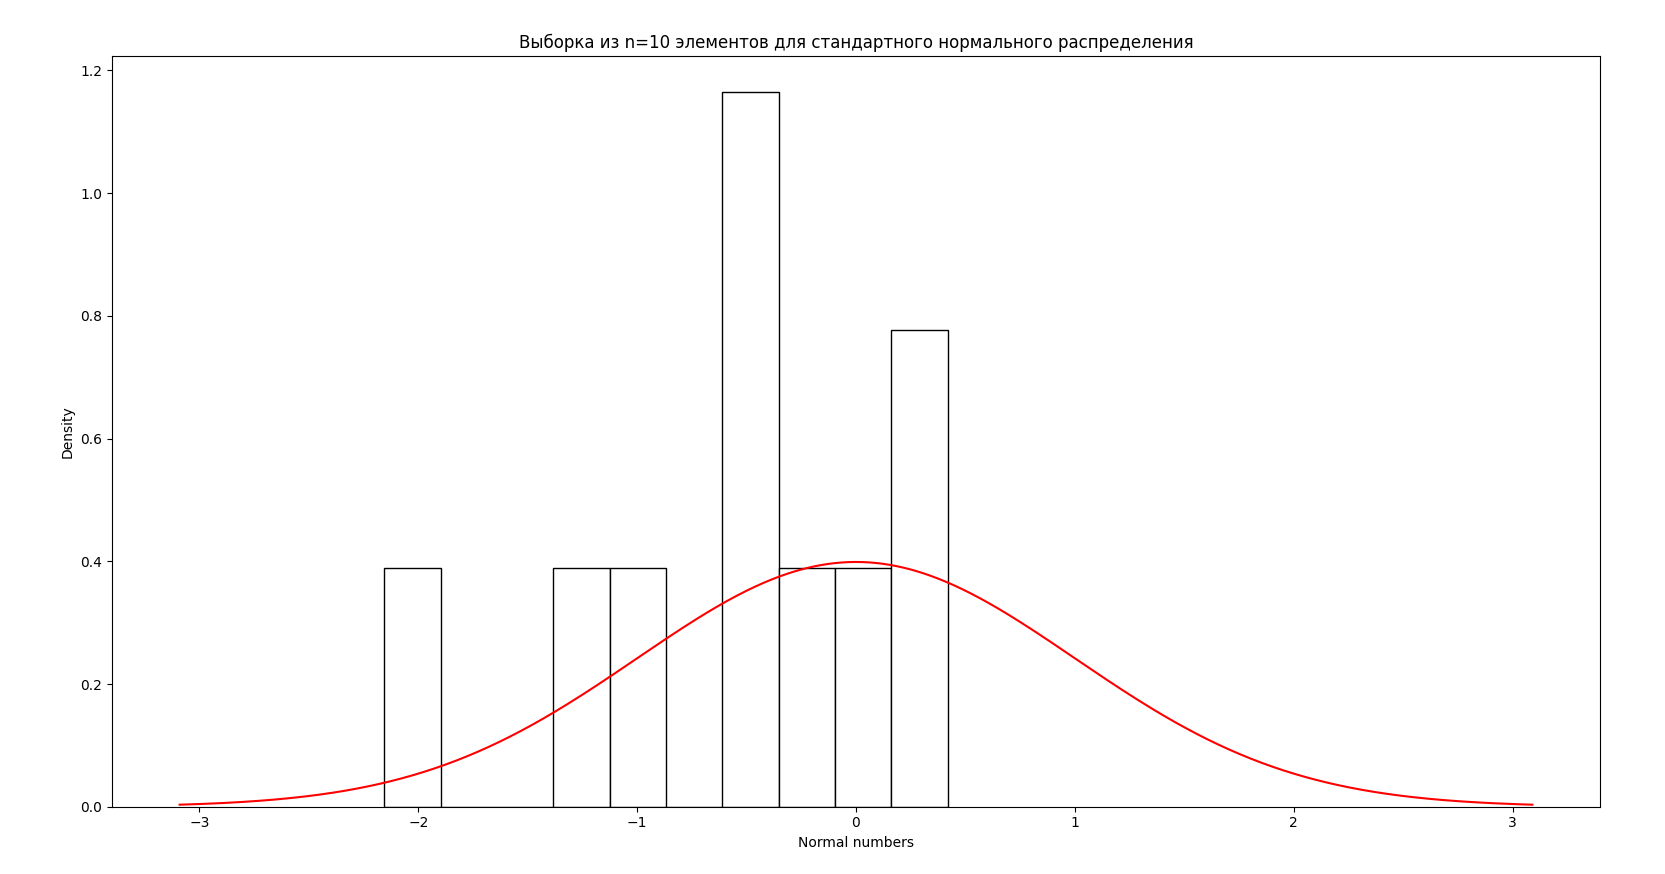
\includegraphics[scale=0.12]{resources/1_gauss_10.png}
		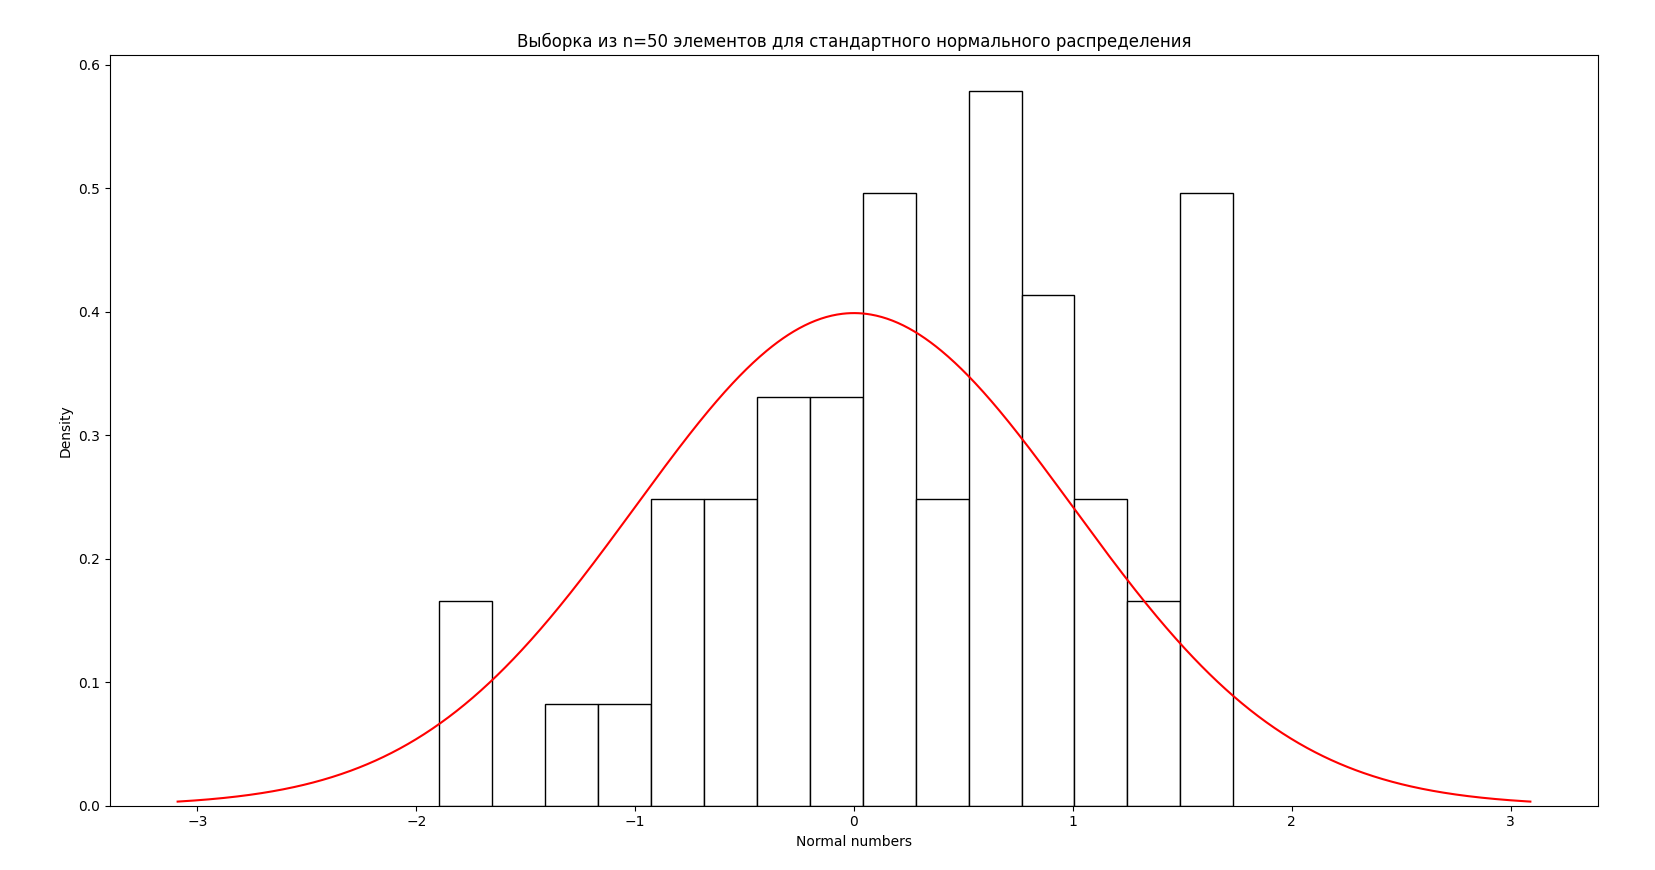
\includegraphics[scale=0.12]{resources/1_gauss_50.png}
		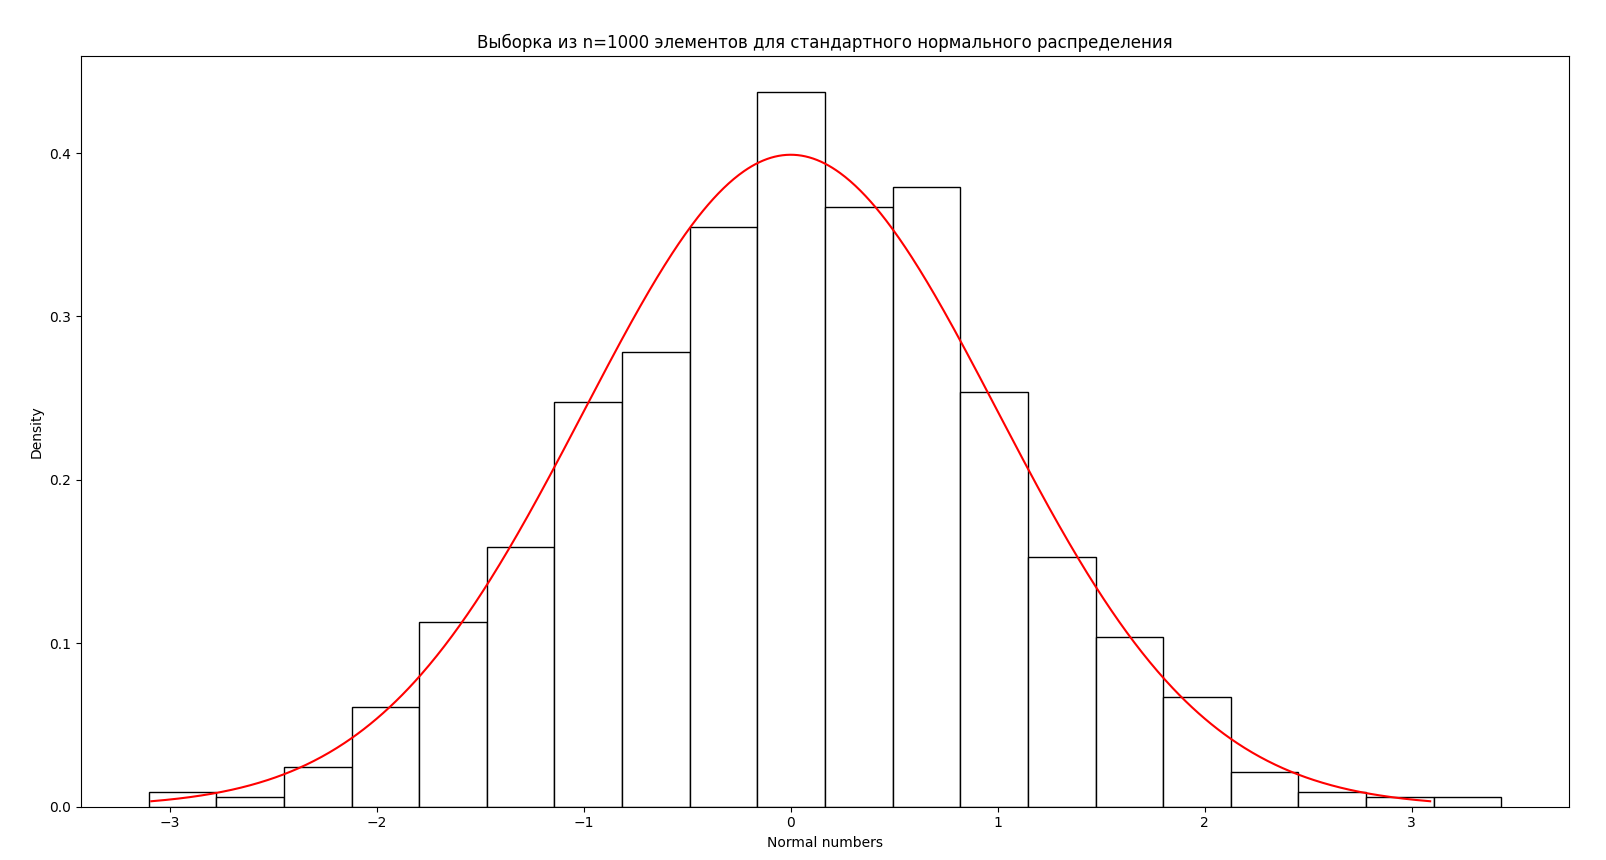
\includegraphics[scale=0.12]{resources/1_gauss_1000.png}
	\end{tabular}
	\caption{Нормальное распределение}
\end{figure}

\begin{figure}[H]
	\begin{tabular}{ccc}
		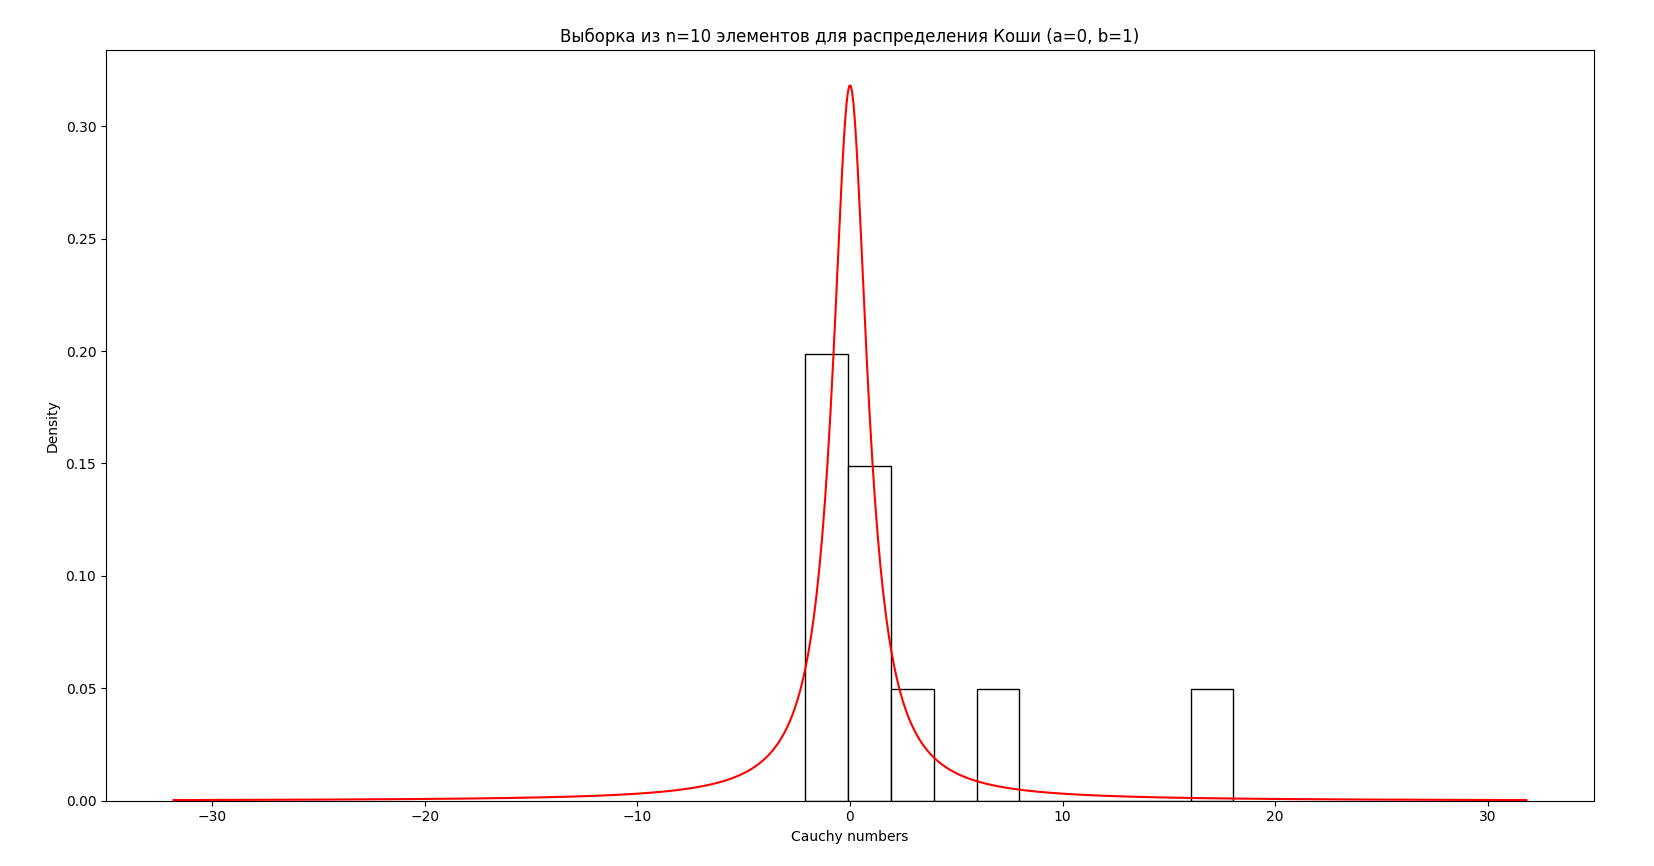
\includegraphics[scale=0.12]{resources/1_cauchy_10.png}
		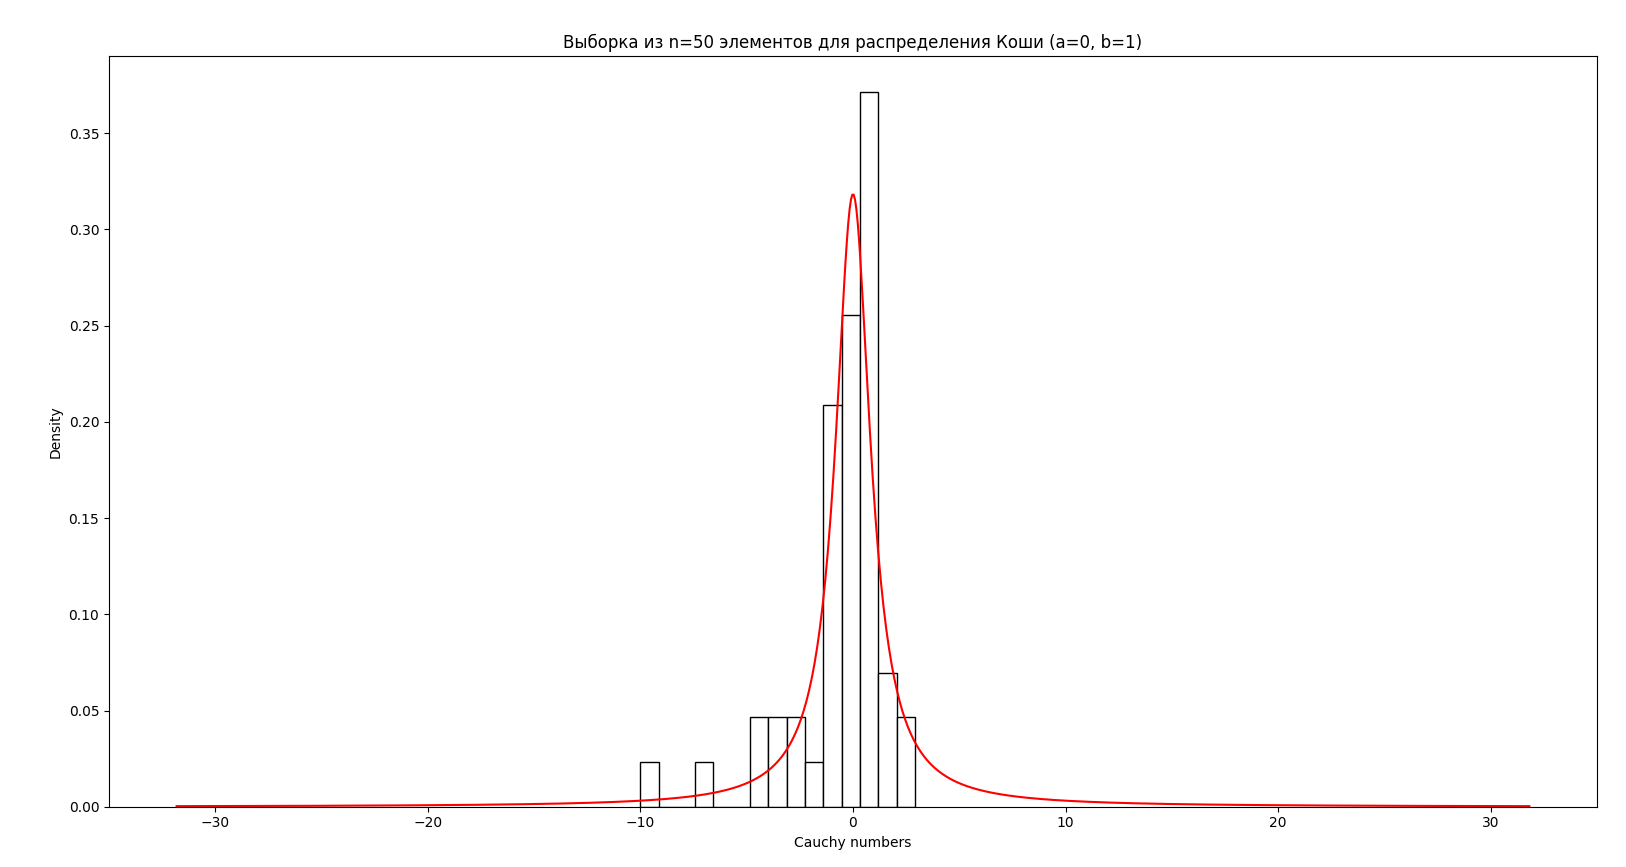
\includegraphics[scale=0.12]{resources/1_cauchy_50.png}
		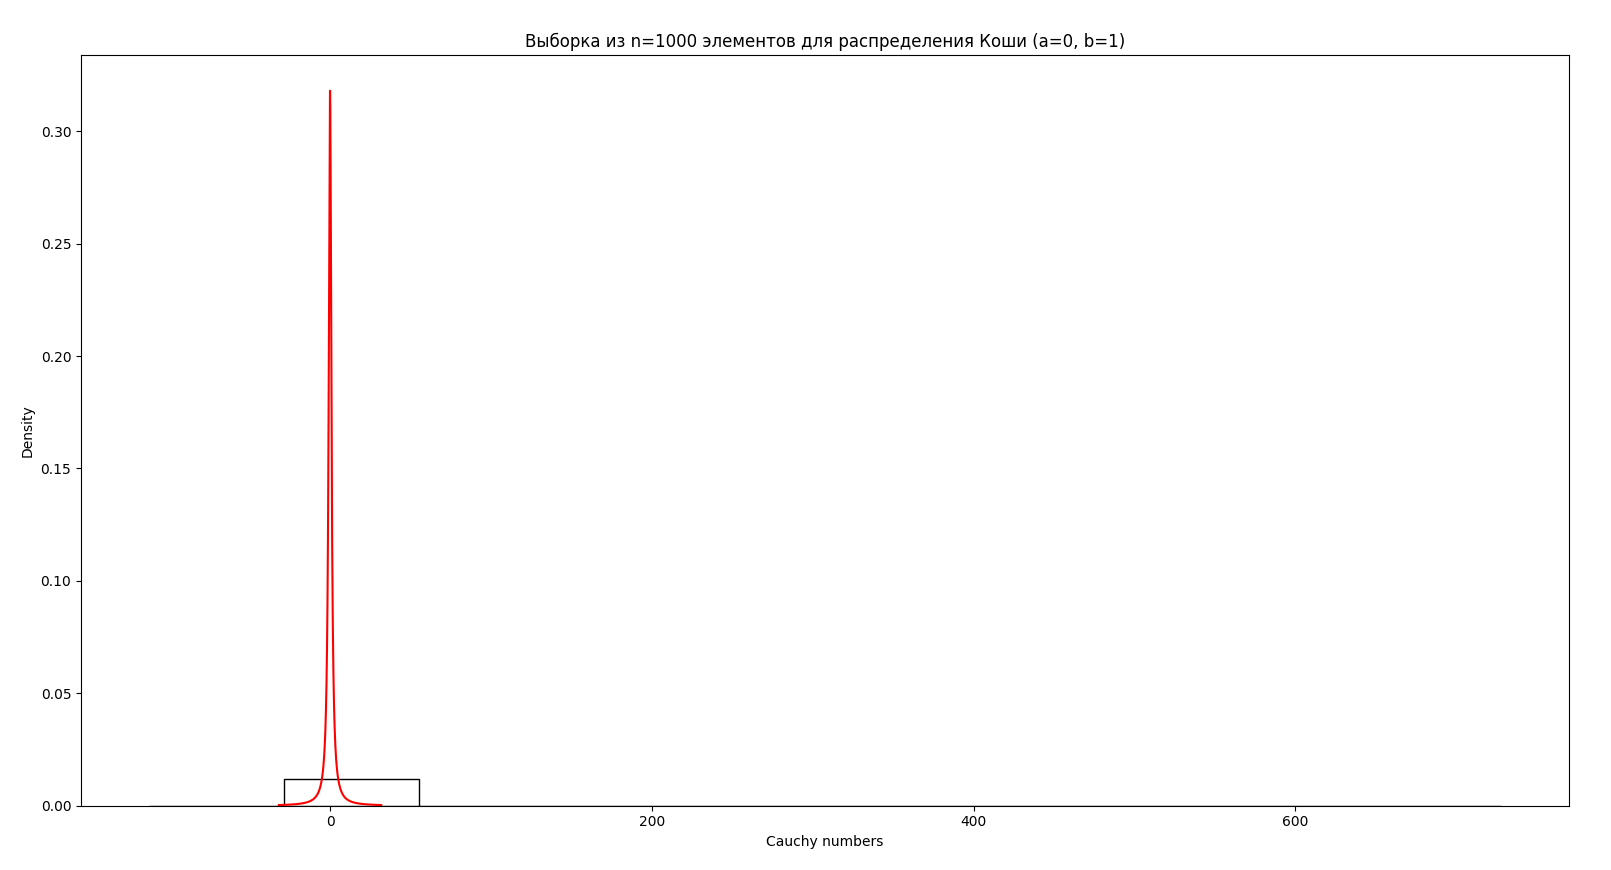
\includegraphics[scale=0.12]{resources/1_cauchy_1000.png}
	\end{tabular}
	\caption{Распределение Коши}
\end{figure}

\begin{figure}[H]
	\begin{tabular}{ccc}
		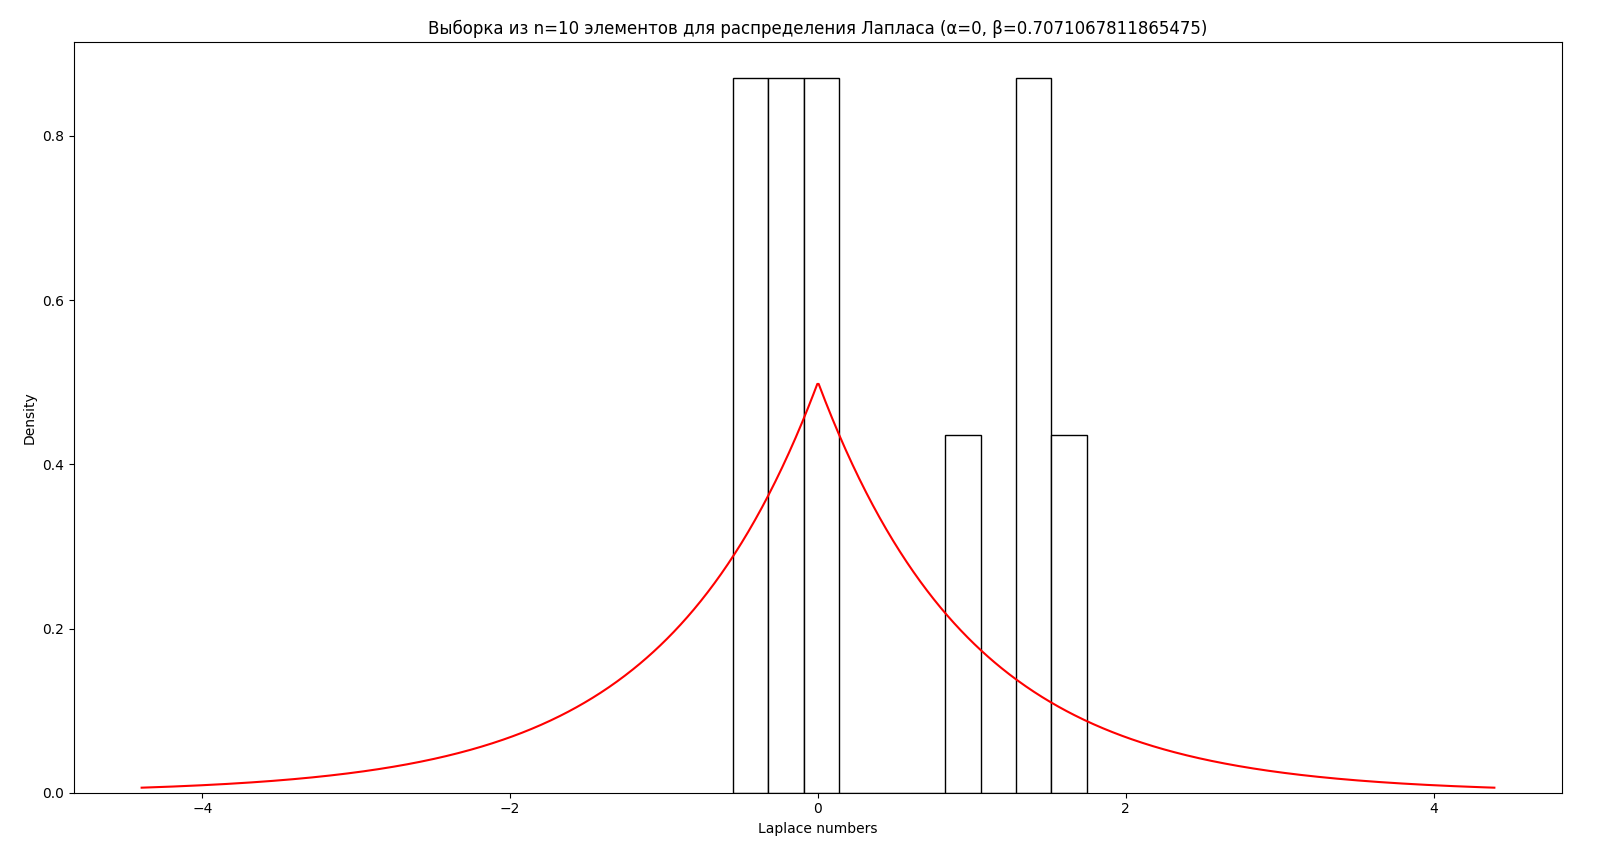
\includegraphics[scale=0.12]{resources/1_laplace_10.png}
		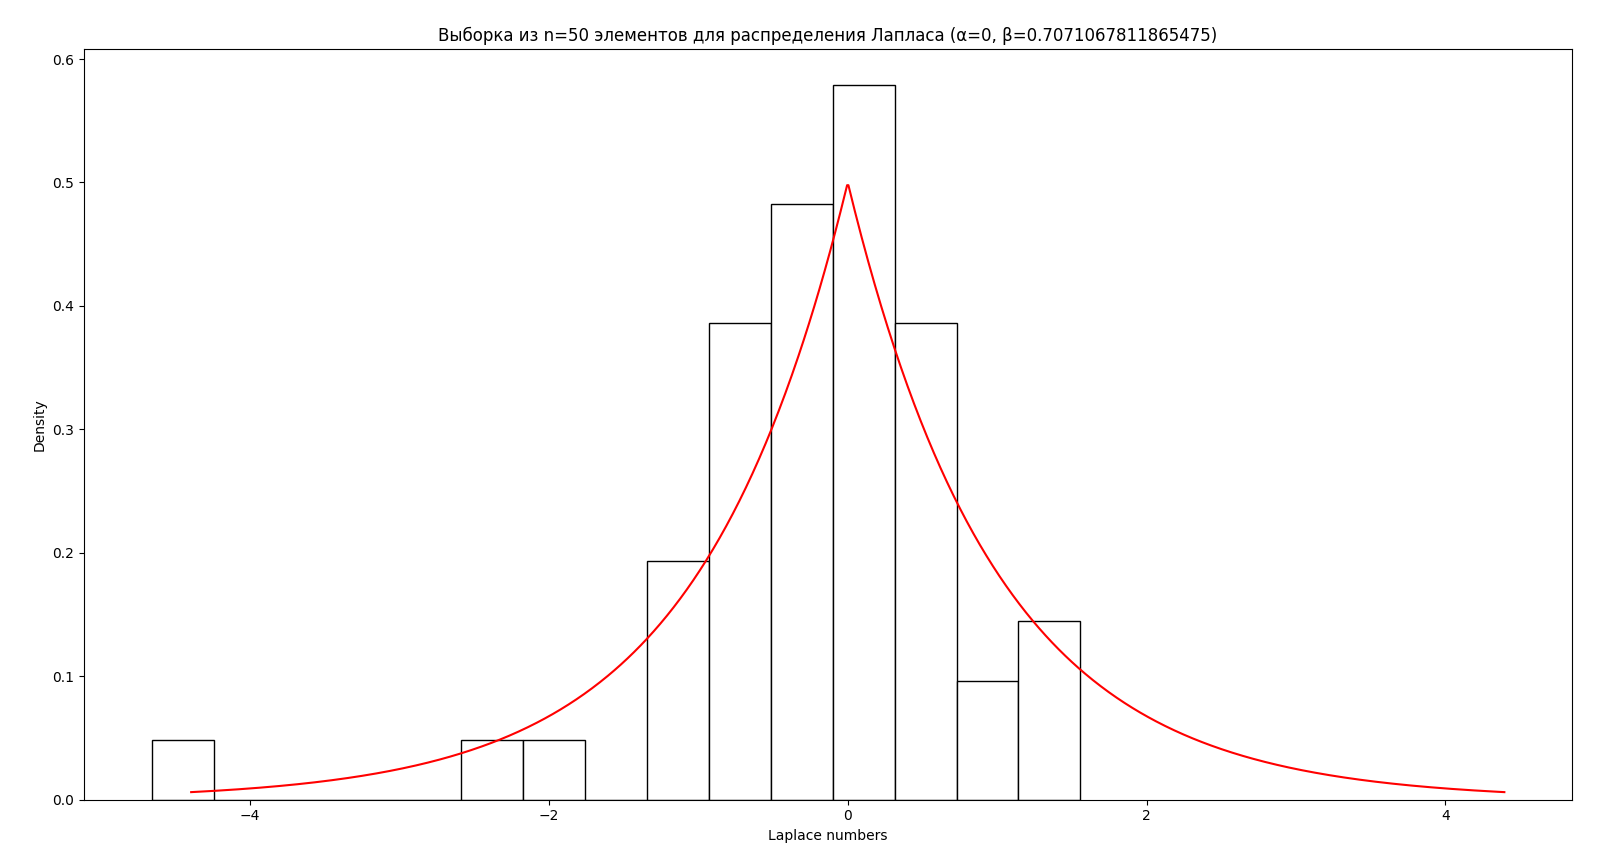
\includegraphics[scale=0.12]{resources/1_laplace_50.png}
		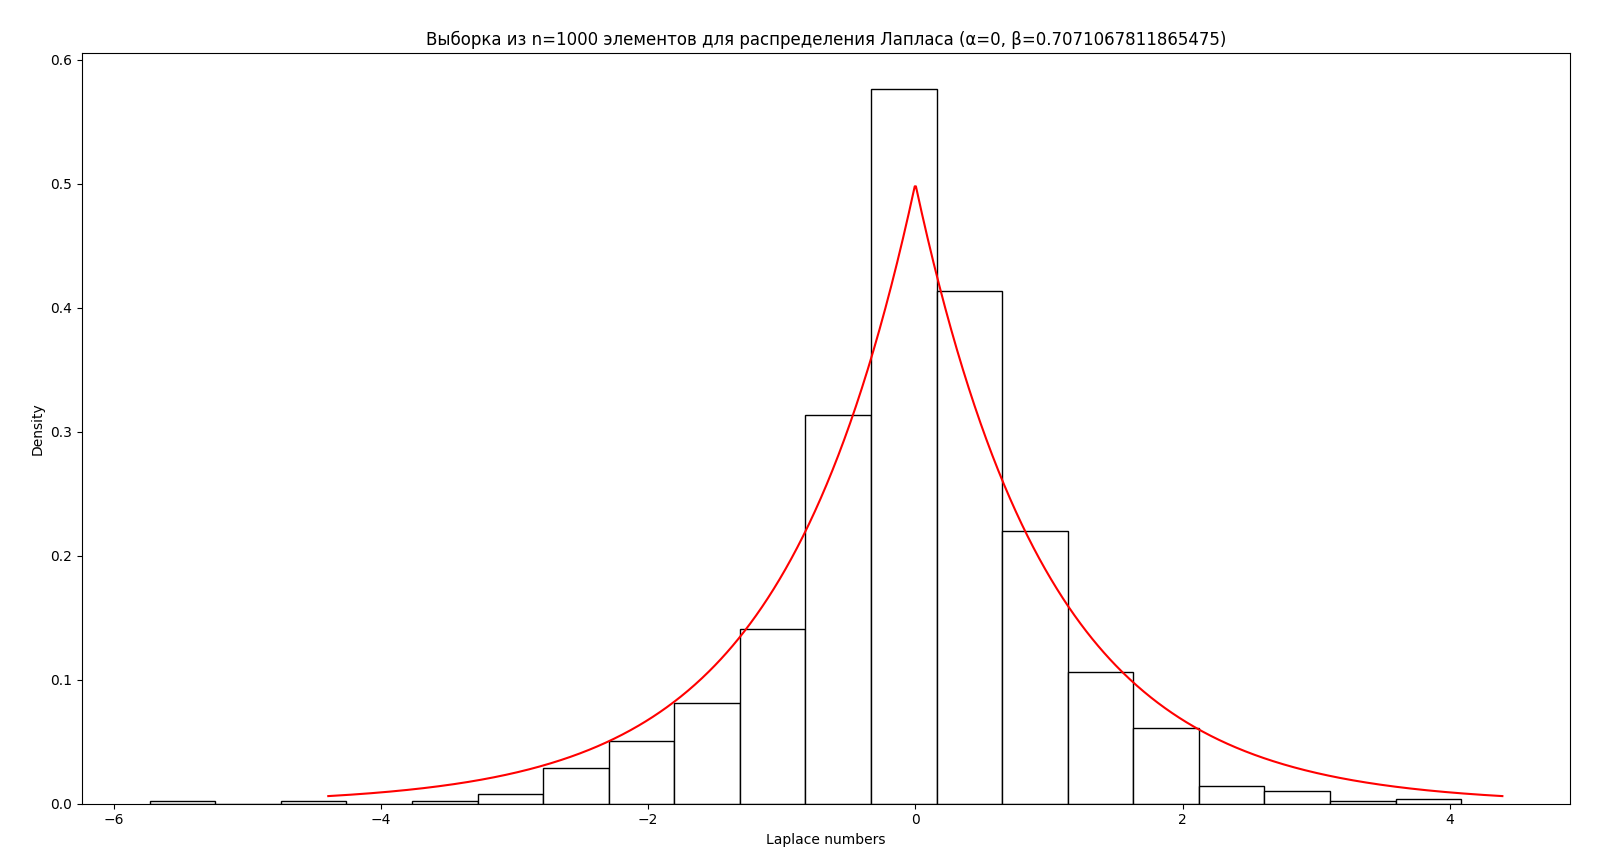
\includegraphics[scale=0.12]{resources/1_laplace_1000.png}
	\end{tabular}
	\caption{Распределение Лапласа}
\end{figure}

\begin{figure}[H]
	\begin{tabular}{ccc}
		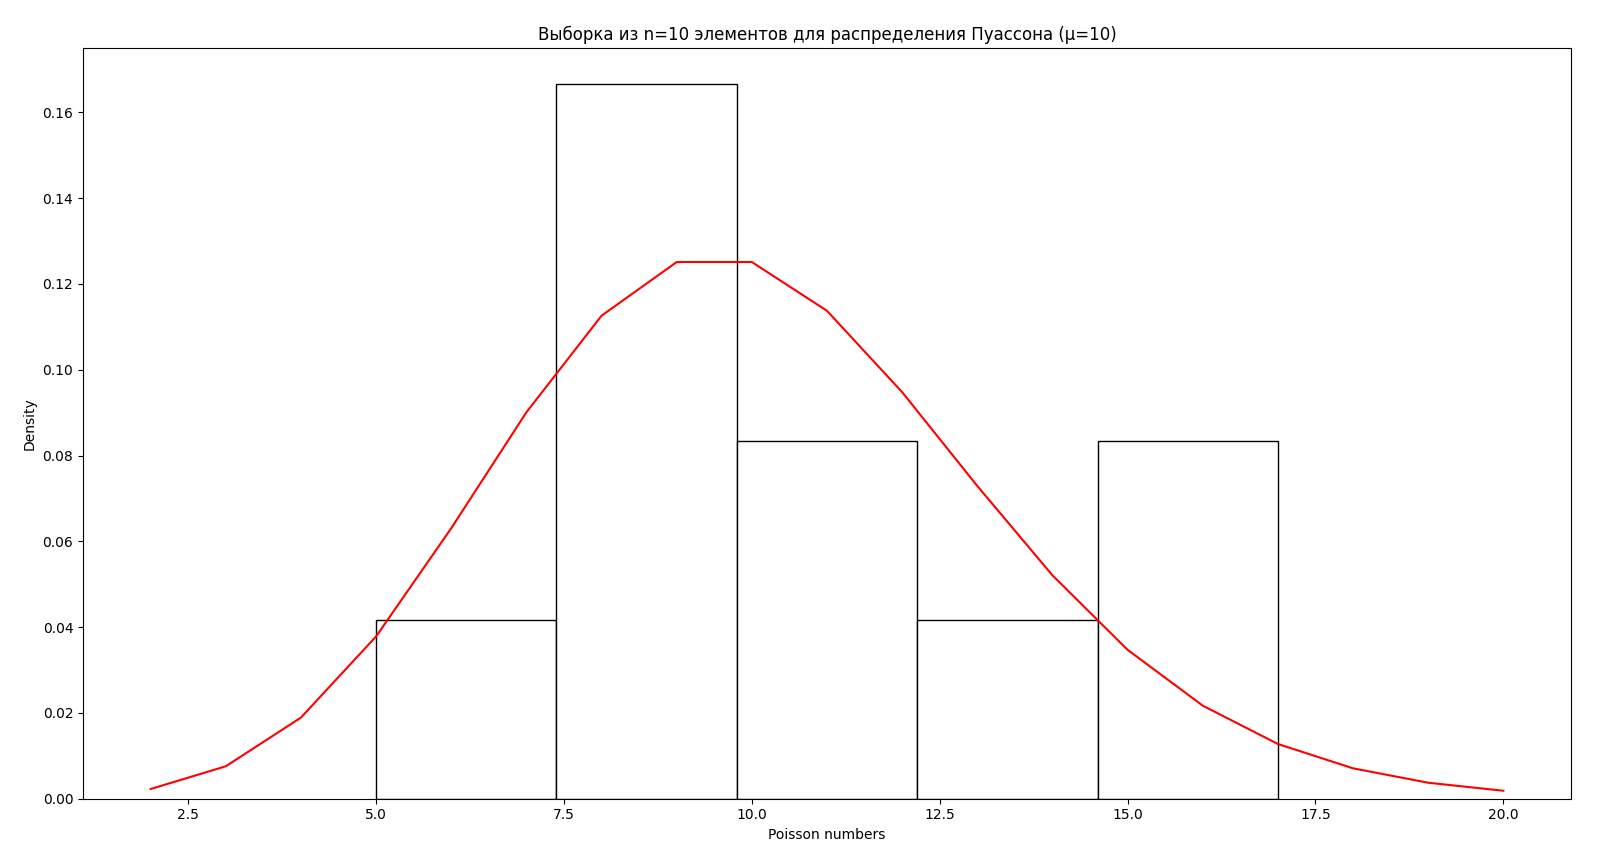
\includegraphics[scale=0.12]{resources/1_poisson_10.png}
		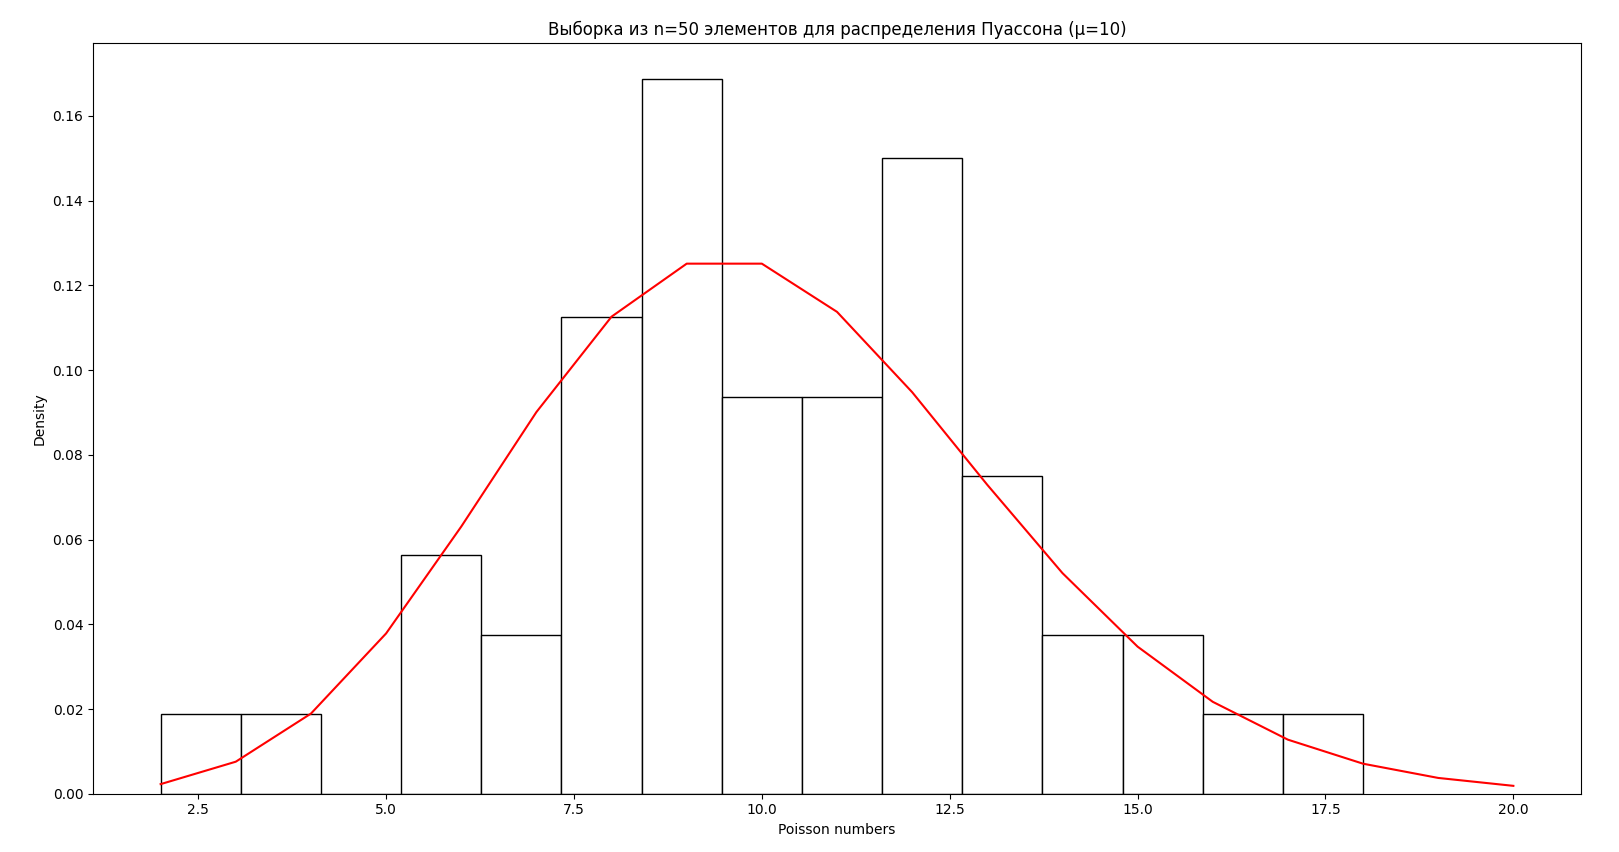
\includegraphics[scale=0.12]{resources/1_poisson_50.png}
		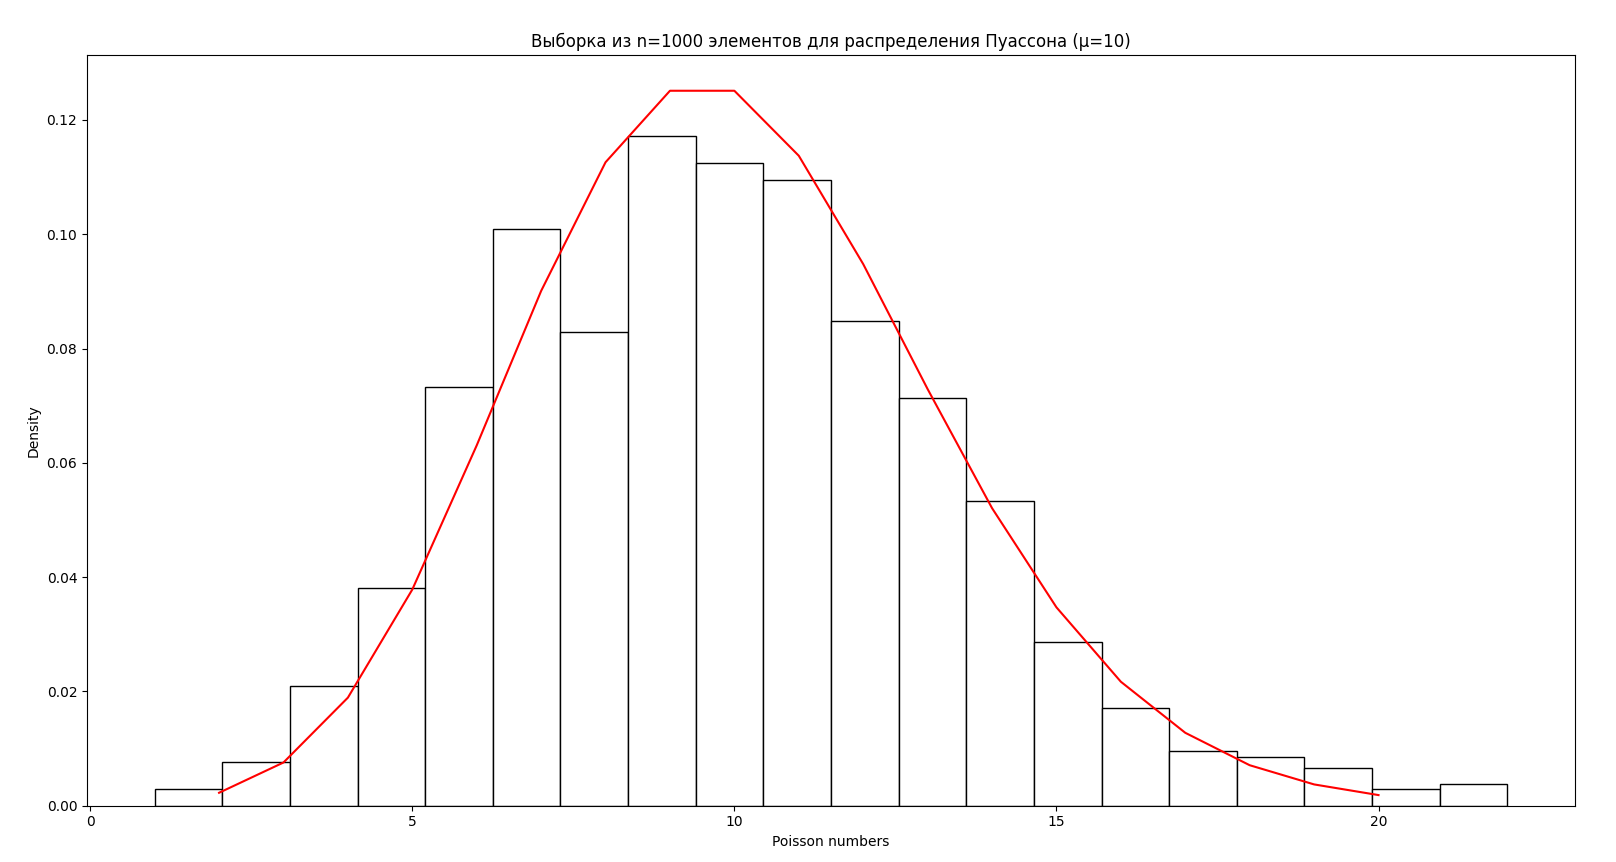
\includegraphics[scale=0.12]{resources/1_poisson_1000.png}
	\end{tabular}
	\caption{Распределение Пуассона}
\end{figure}


\begin{figure}[H]
	\begin{tabular}{ccc}
		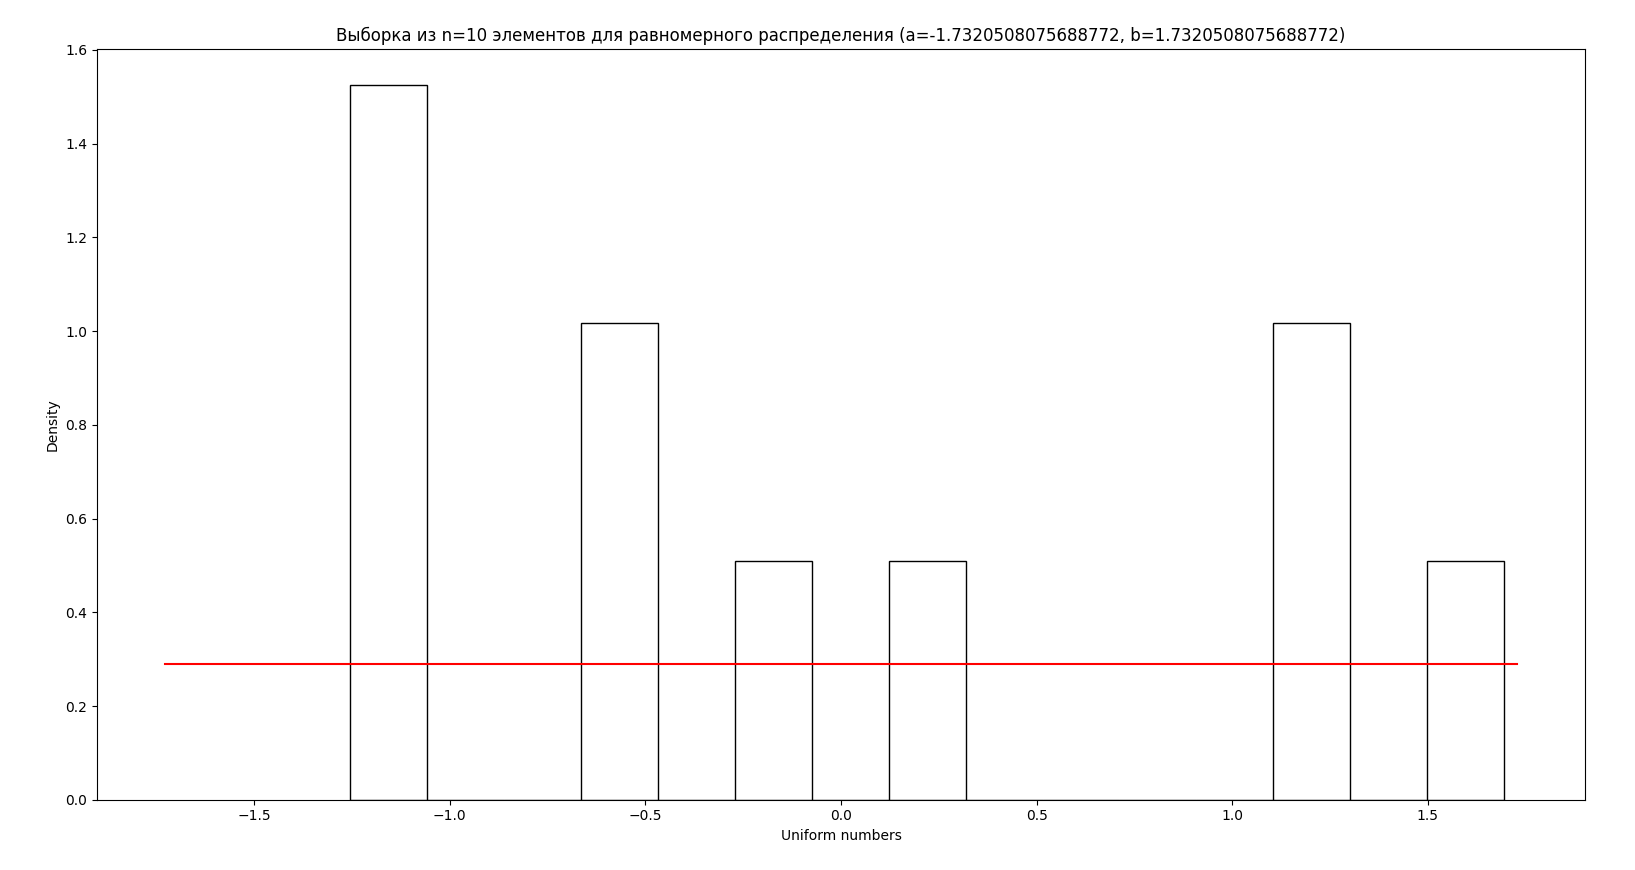
\includegraphics[scale=0.12]{resources/1_uniform_10.png}
		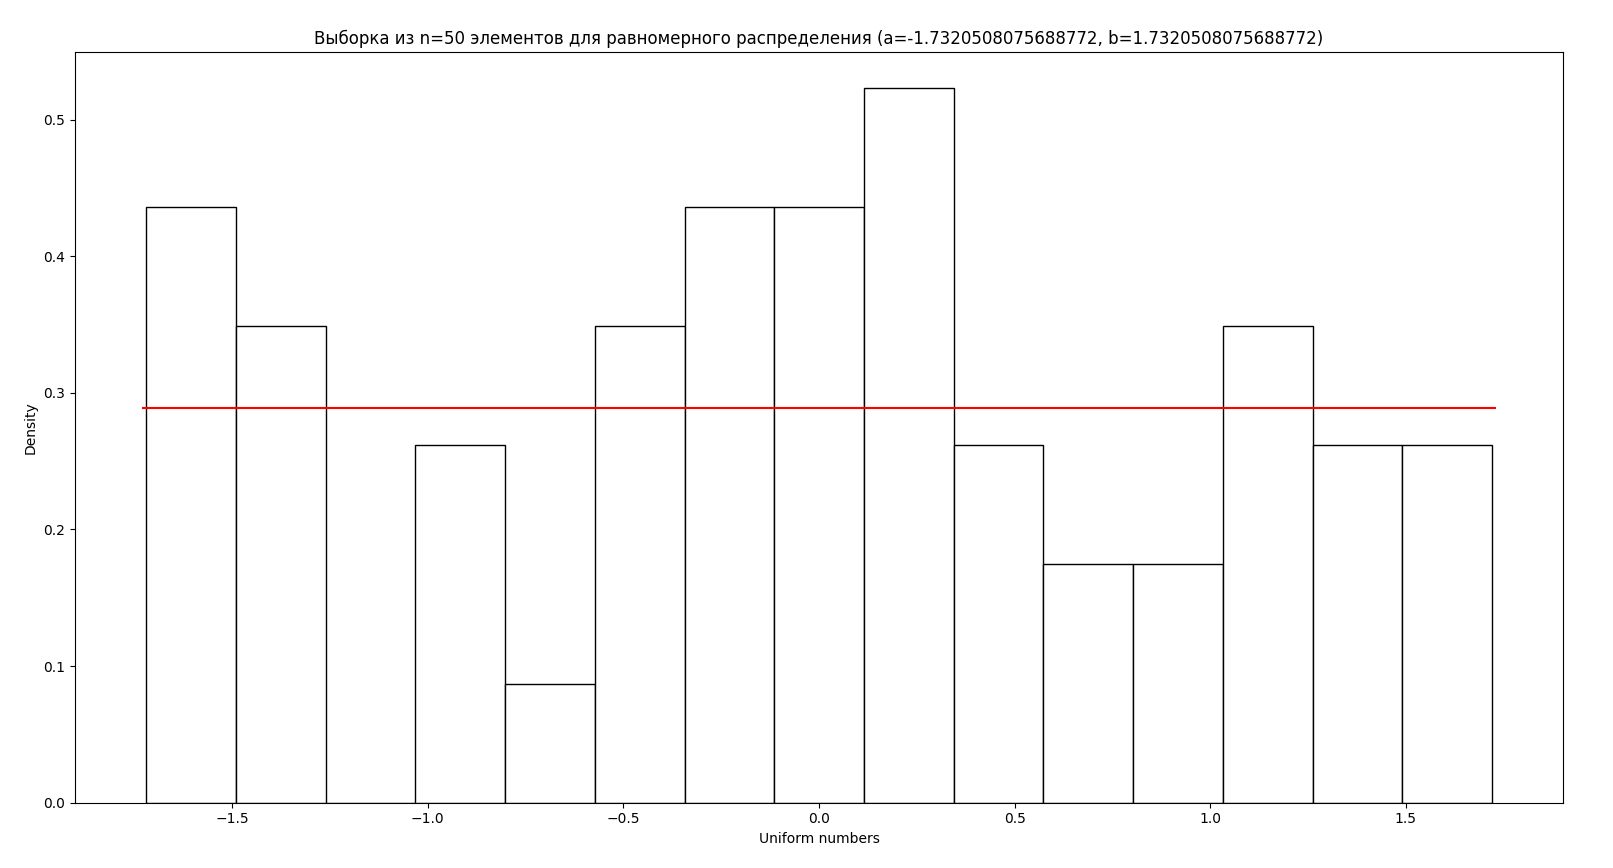
\includegraphics[scale=0.12]{resources/1_uniform_50.png}
		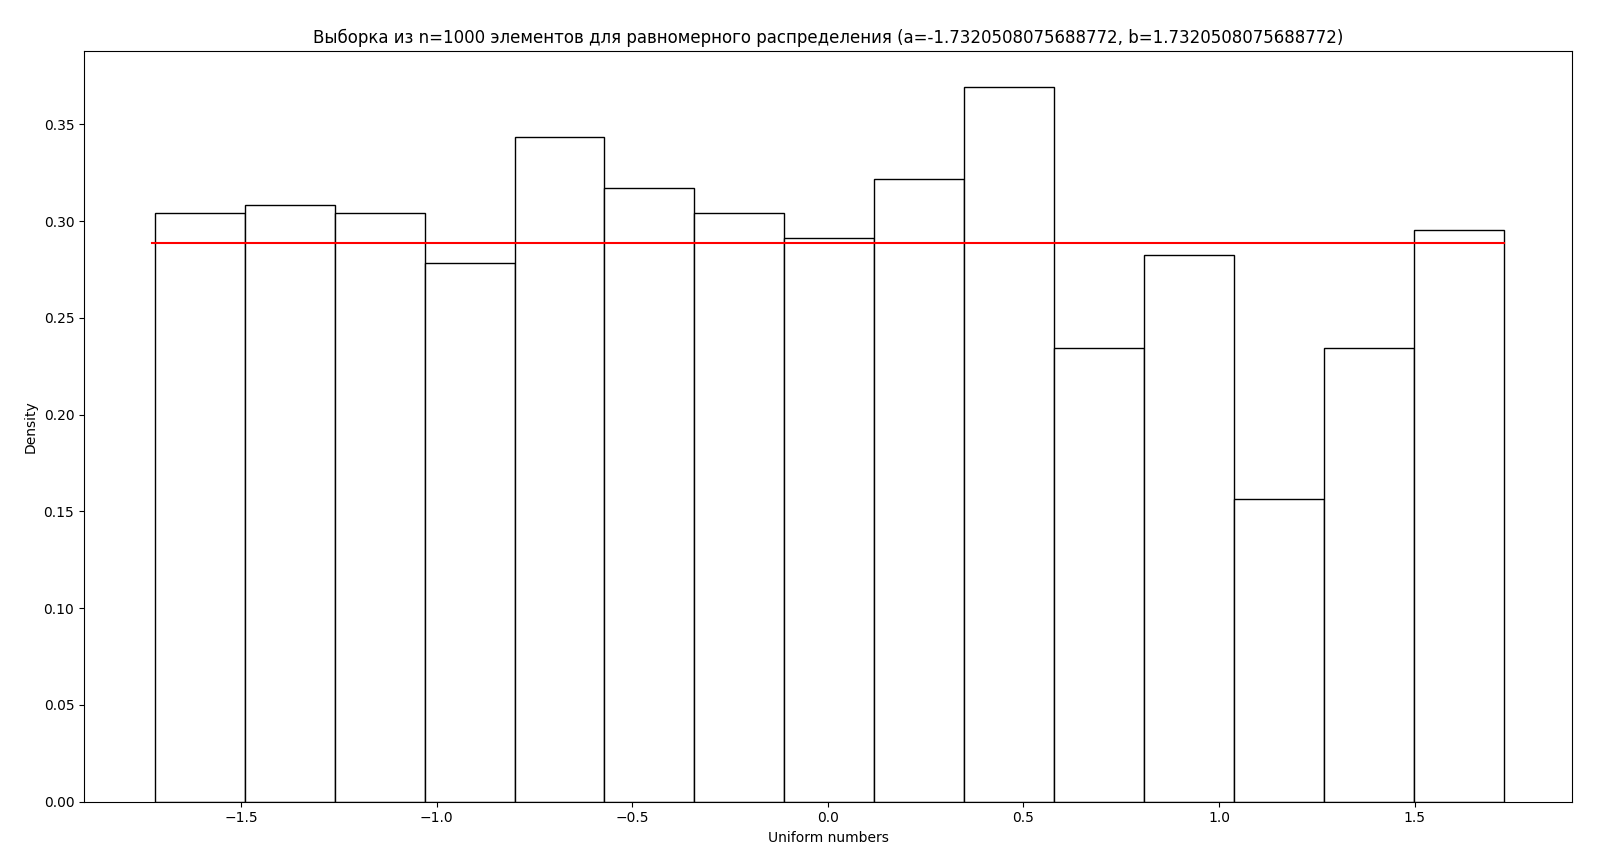
\includegraphics[scale=0.12]{resources/1_uniform_1000.png}
	\end{tabular}
	\caption{Равномерное распределение}
\end{figure}

\subsection{Характеристики положения и рассеяния}

Как было проведено округление: \\
В оценке $x = E \pm \sqrt D$ вариации подлежит первая цифра после точки.  \\
В данном случае $𝑥 = 0.0 \pm 0.1𝑘$  где, $k$ − зависит от доверительной вероятности и вида распределения (рассматривается в дальнейшем цикле лабораторных работ). \\
Округление сделано для $k = 1$.

\begin{table}[H]
	\begin{center}
		\begin{tabular}{|c||c|c|c|c|c|}
			\hline
			normal n=10 & $\overline{x} $ & $med\:x$ & $z_{R}$ & $z_{Q}$ & $z_{tr}$ \\
			\hline\hline
			$E(z)$ & -0.001 & 0.001 & -0.010 & -0.003 & -0.000 \\
			\hline
			$D(z)$ & 0.001 & 0.001 & 0.064 & 0.001 & 0.001 \\
			\hline
			$E(z) \pm \sqrt{D(z)}$ & [-0.033;0.031]  & [-0.031;0.033]  & [-0.263;0.243]  & [-0.035;0.029]  & [-0.032;0.032] \\
			\hline
			$\hat{E}(z)$ & 0.0 & 0.0 & 0.0\pm 0.2 & 0.0 & 0.0 \\
			\hline\hline
			normal n=100 & $\overline{x} $ & $med\:x$ & $z_{R}$ & $z_{Q}$ & $z_{tr}$ \\
			\hline\hline
			$E(z)$ & 0.003 & 0.125 & -0.005 & 0.005 & 0.005 \\
			\hline
			$D(z)$ & 0.096 & 0.153 & 0.183 & 0.110 & 0.108  \\
			\hline
			$E(z) \pm \sqrt{D(z)}$ & [-0.307;0.313]  & [-0.266;0.516]  & [-0.433;0.423]  & [-0.327;0.337]  & [-0.324;0.334] \\
			\hline
			$\hat{E}(z)$ & 0.0\pm 0.3 & 0.1\pm 0.4 & 0.0\pm 0.4 & 0.0\pm 0.3 & 0.0\pm 0.3 \\
			\hline\hline
			normal n=1000 & $\overline{x} $ & $med\:x$ & $z_{R}$ & $z_{Q}$ & $z_{tr}$ \\
			\hline\hline
			$E(z)$ & 0.000 & 0.012 & 0.001 & -0.016 & -0.000 \\
			\hline
			$D(z)$ & 0.010 & 0.016 & 0.095 & 0.012 & 0.012 \\
			\hline
			$E(z) \pm \sqrt{D(z)}$ & [-0.100;0.100]  & [-0.114;0.138]  & [-0.307;0.309]  & [-0.126;0.094]  & [-0.110;0.110] \\
			\hline
			$\hat{E}(z)$ & 0.0\pm 0.1 & 0.0\pm 0.1 & 0.0\pm 0.3 & 0.0\pm 0.1 & 0.0\pm 0.1 \\
			\hline
		\end{tabular}
	\end{center}
	\caption{Характеристики положения и рассеяния нормального распределения}
\end{table} 

\begin{table}[H]
	\begin{center}
		\begin{tabular}{|c||c|c|c|c|c|}
			\hline
			cauchy n=10 & $\overline{x} $ & $med\:x$ & $z_{R}$ & $z_{Q}$ & $z_{tr}$ \\
			\hline\hline
			$E(z)$ & 2.060 & 0.006 & 1048.226 & 0.002 & 0.005 \\
			\hline
			$D(z)$ & 1601.013 & 0.002 & 397755994.462 & 0.005 & 0.003 \\
			\hline
			$E(z) \pm \sqrt{D(z)}$ & [-37.953;42.073]  & [-0.039;0.051]  & [-18895.595;20992.047]  & [-0.069;0.073]  & [-0.050;0.060] \\
			\hline
			$\hat{E}(z)$ & 2.1\pm 40.0 & 0.0 & - & 0.0\pm 0.1 & 0.0\pm 0.1 \\
			\hline\hline
			cauchy n=100 & $\overline{x} $ & $med\:x$ & $z_{R}$ & $z_{Q}$ & $z_{tr}$ \\
			\hline\hline
			$E(z)$ & 0.292 & 0.140 & 1.274 & -0.036 & -0.039 \\
			\hline
			$D(z)$ & 548.952 & 0.312 & 13233.118 & 1.245 & 0.447 \\
			\hline
			$E(z) \pm \sqrt{D(z)}$ & [-23.138;23.722]  & [-0.419;0.699]  & [-113.761;116.309]  & [-1.152;1.080]  & [-0.708;0.630] \\
			\hline
			$\hat{E}(z)$ & - & 0.1\pm0.6 & - & 0.0\pm 1.1 & 0.0\pm 0.7 \\
			\hline\hline
			cauchy n=1000 & $\overline{x} $ & $med\:x$ & $z_{R}$ & $z_{Q}$ & $z_{tr}$ \\
			\hline\hline
			$E(z)$ & 0.317 & 0.009 & 14.999 & -0.040 & -0.004 \\
			\hline
			$D(z)$ & 622.907 & 0.026 & 1520986.297 & 0.055 & 0.027 \\
			\hline
			$E(z) \pm \sqrt{D(z)}$ & [-24.641;25.275]  & [-0.152;0.170]  & [-1218.284;1248.282]  & [-0.275;0.195]  & [-0.168;0.160] \\
			\hline
			$\hat{E}(z)$ & - & 0.0\pm 0.2 & - & 0.0\pm 0.2 & 0.0\pm 0.2 \\
			\hline
		\end{tabular}
	\end{center}
	\caption{Характеристики положения и рассеяния распределения Коши}
\end{table}

\begin{table}[H]
	\begin{center}
		\begin{tabular}{|c||c|c|c|c|c|}
			\hline
			laplace n=10 & $\overline{x} $ & $med\:x$ & $z_{R}$ & $z_{Q}$ & $z_{tr}$ \\
			\hline\hline
			$E(z)$ & -0.001 & -0.000 & -0.011 & -0.002 & -0.001 \\
			\hline
			$D(z)$ & 0.001 & 0.001 & 0.410 & 0.001 & 0.001 \\
			\hline
			$E(z) \pm \sqrt{D(z)}$ & [-0.033;0.031]  & [-0.032;0.032]  & [-0.651;0.629]  & [-0.034;0.030]  & [-0.033;0.031] \\
			\hline
			$\hat{E}(z)$ & 0.0 & 0.0 & 0.0\pm 0.7 & 0.0 & 0.0 \\
			\hline\hline
			laplace n=100 & $\overline{x} $ & $med\:x$ & $z_{R}$ & $z_{Q}$ & $z_{tr}$ \\
			\hline\hline
			$E(z)$ & 0.003 & 0.091 & 0.013 & -0.004 & 0.000 \\
			\hline
			$D(z)$ & 0.104 & 0.082 & 0.377 & 0.108 & 0.077 \\
			\hline
			$E(z) \pm \sqrt{D(z)}$ & [-0.319;0.325]  & [-0.195;0.377]  & [-0.601;0.627]  & [-0.333;0.325]  & [-0.277;0.277] \\
			\hline
			$\hat{E}(z)$ & 0.0\pm 0.3 & 0.1\pm 0.3 & 0.0\pm 0.6 & 0.0\pm 0.3 & 0.0\pm 0.3 \\
			\hline\hline
			laplace n=1000 & $\overline{x} $ & $med\:x$ & $z_{R}$ & $z_{Q}$ & $z_{tr}$ \\
			\hline\hline
			$E(z)$ & 0.003 & 0.011 & -0.018 & -0.008 & 0.004 \\
			\hline
			$D(z)$ & 0.010 & 0.006 & 0.386 & 0.010 & 0.006 \\
			\hline
			$E(z) \pm \sqrt{D(z)}$ & [-0.097;0.103]  & [-0.066;0.088]  & [-0.639;0.603]  & [-0.108;0.092]  & [-0.073;0.081] \\
			\hline
			$\hat{E}(z)$ & 0.0\pm 0.1 & 0.0\pm 0.1 & 0.0\pm 0.6 & 0.0\pm 0.1 & 0.0\pm 0.1 \\
			\hline
		\end{tabular}
	\end{center}
	\caption{Характеристики положения и рассеяния распределения Лапласа}
\end{table} 

\begin{table}[H]
	\begin{center}
		\begin{tabular}{|c||c|c|c|c|c|}
			\hline
			poisson n=10 & $\overline{x} $ & $med\:x$ & $z_{R}$ & $z_{Q}$ & $z_{tr}$ \\
			\hline\hline
			$E(z)$ & 9.997 & 9.992 & 11.669 & 9.993 & 9.857 \\
			\hline
			$D(z)$ & 0.010 & 0.008 & 0.666 & 0.003 & 0.011 \\
			\hline
			$E(z) \pm \sqrt{D(z)}$ & [9.897;10.097]  & [9.903;10.081]  & [10.853;12.485]  & [9.938;10.048]  & [9.752;9.962] \\
			\hline
			$\hat{E}(z)$ & 10.0\pm 0.1 & 10.0\pm 0.1 & 11.7\pm 0.8 & 10.0\pm 0.1 & 9.9\pm 0.1 \\
			\hline\hline
			poisson n=100 & $\overline{x} $ & $med\:x$ & $z_{R}$ & $z_{Q}$ & $z_{tr}$ \\
			\hline\hline
			$E(z)$ & 10.014 & 10.242 & 10.309 & 9.950 & 9.902 \\
			\hline
			$D(z)$ & 1.086 & 1.671 & 1.917 & 1.287 & 1.186 \\
			\hline
			$E(z) \pm \sqrt{D(z)}$ & [8.972;11.056]  & [8.949;11.535]  & [8.924;11.694]  & [8.816;11.084]  & [8.813;10.991] \\
			\hline
			$\hat{E}(z)$ & 10.0\pm 1.0 & 10.2\pm 1.3 & 10.3\pm 1.4 & 9.9\pm 1.1 & 9.9\pm 1.1 \\
			\hline\hline
			poisson n=1000 & $\overline{x} $ & $med\:x$ & $z_{R}$ & $z_{Q}$ & $z_{tr}$ \\
			\hline\hline
			$E(z)$ & 9.995 & 9.873 & 10.925 & 9.864 & 9.855 \\
			\hline
			$D(z)$ & 0.093 & 0.197 & 1.123 & 0.153 & 0.117 \\
			\hline
			$E(z) \pm \sqrt{D(z)}$ & [9.690;10.300]  & [9.429;10.317]  & [9.865;11.985]  & [9.473;10.255]  & [9.513;10.197] \\
			\hline
			$\hat{E}(z)$ & 10.0\pm 0.3 & 9.9\pm 0.5 & 10.9\pm 1.0 & 9.9\pm 0.4 & 9.9\pm 0.3 \\
			\hline
		\end{tabular}
	\end{center}
	\caption{Характеристики положения и рассеяния распределения Пуассона}
\end{table} 

\begin{table}[H]
	\begin{center}
		\begin{tabular}{|c||c|c|c|c|c|}
			\hline
			uniform n=10 & $\overline{x} $ & $med\:x$ & $z_{R}$ & $z_{Q}$ & $z_{tr}$ \\
			\hline\hline
			$E(z)$ & 0.001 & 0.003 & -0.000 & -0.001 & 0.001 \\
			\hline
			$D(z)$ & 0.001 & 0.003 & 0.000 & 0.002 & 0.002 \\
			\hline
			$E(z) \pm \sqrt{D(z)}$ & [-0.031;0.033]  & [-0.052;0.058]  & [-0.000;0.000]  & [-0.046;0.044]  & [-0.044;0.046] \\
			\hline
			$\hat{E}(z)$ & 0.0 & 0.0 & 0.0 & 0.0 & 0.0 \\
			\hline\hline
			uniform n=100 & $\overline{x} $ & $med\:x$ & $z_{R}$ & $z_{Q}$ & $z_{tr}$ \\
			\hline\hline
			$E(z)$ & -0.004 & 0.142 & 0.002 & -0.003 & -0.007 \\
			\hline
			$D(z)$ & 0.101 & 0.244 & 0.045 & 0.139 & 0.163 \\
			\hline
			$E(z) \pm \sqrt{D(z)}$ & [-0.322;0.314]  & [-0.352;0.636]  & [-0.210;0.214]  & [-0.376;0.370]  & [-0.411;0.397] \\
			\hline
			$\hat{E}(z)$ & 0.0\pm 0.3 & 0.1\pm 0.5 & 0.0\pm 0.2 & 0.0\pm 0.4 & 0.0\pm 0.4 \\
			\hline\hline
			uniform n=1000 & $\overline{x} $ & $med\:x$ & $z_{R}$ & $z_{Q}$ & $z_{tr}$ \\
			\hline\hline
			$E(z)$ & -0.007 & 0.006 & -0.003 & -0.022 & -0.008 \\
			\hline
			$D(z)$ & 0.011 & 0.031 & 0.001 & 0.016 & 0.021 \\
			\hline
			$E(z) \pm \sqrt{D(z)}$ & [-0.112;0.098]  & [-0.170;0.182]  & [-0.035;0.029]  & [-0.148;0.104]  & [-0.153;0.137] \\
			\hline
			$\hat{E}(z)$ & 0.0\pm 0.1 & 0.0\pm 0.2 & 0.0 & 0.0\pm 0.1 & 0.0\pm 0.2 \\
			\hline
		\end{tabular}
	\end{center}
	\caption{Характеристики положения и рассеяния равномерного распределения}
\end{table}

\subsection{Боксплот Тьюки}

\begin{figure}[H]
	\centering
	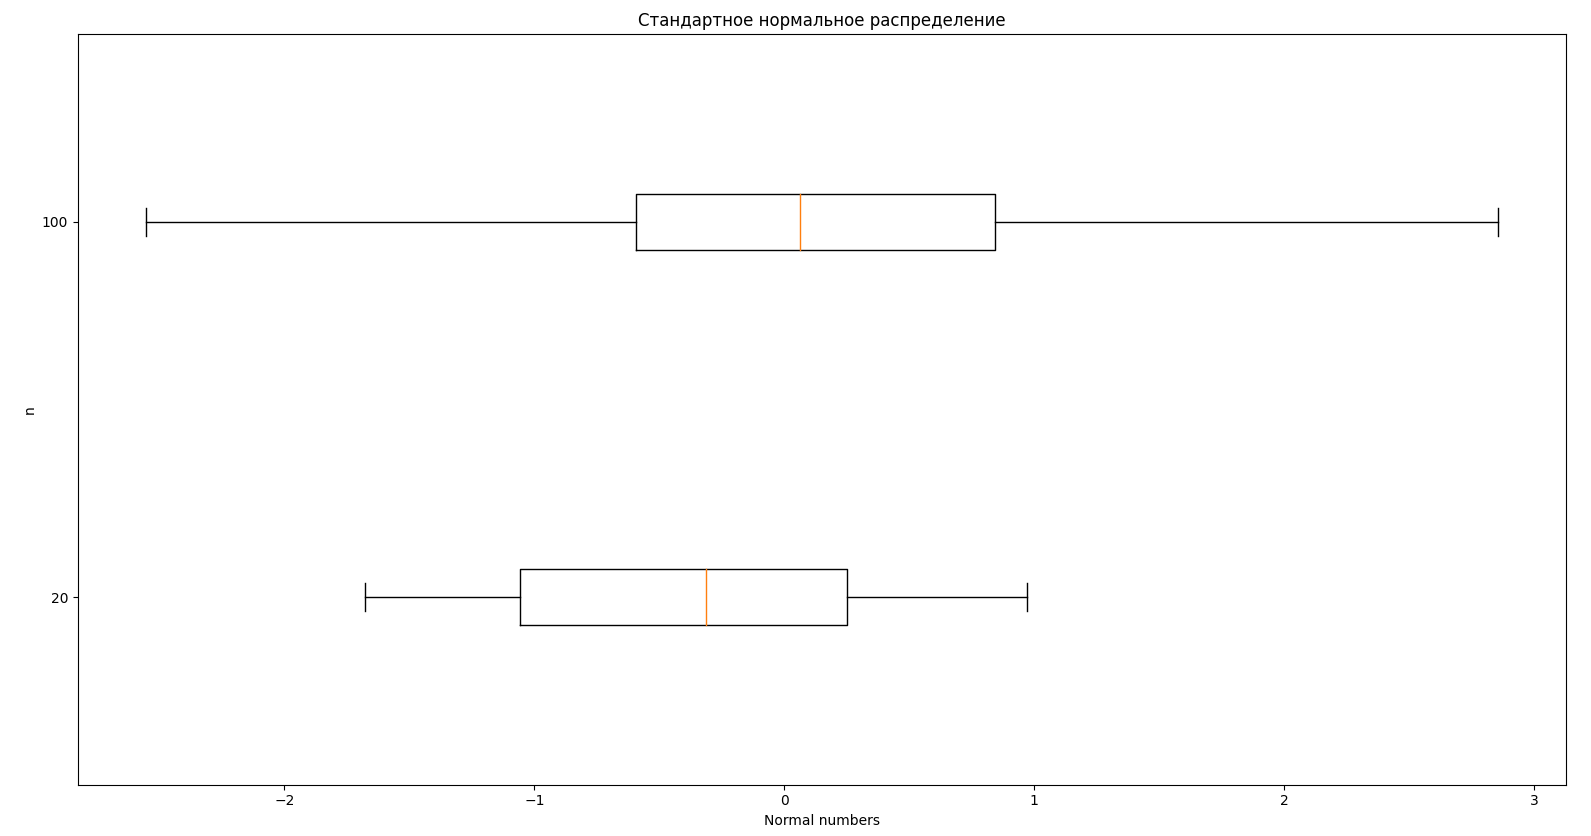
\includegraphics[scale=0.3]{resources/3_gauss.png}
	\caption{Боксплот нормального распределения}
\end{figure}

\begin{figure}[H]
	\centering
	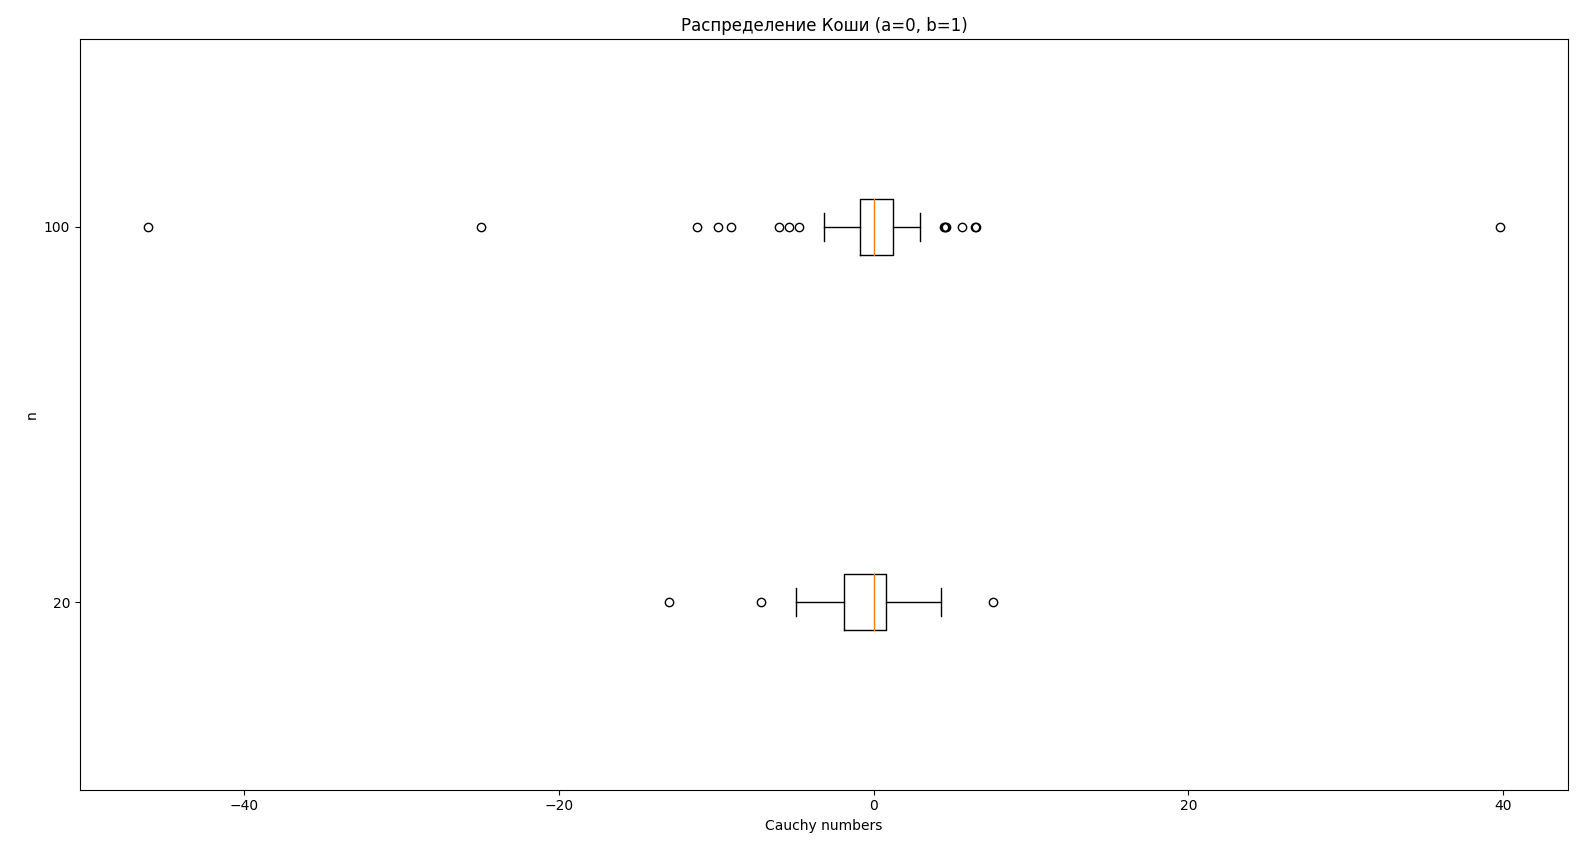
\includegraphics[scale=0.3]{resources/3_cauchy.png}
	\caption{Боксплот распределения Коши}
\end{figure}

\begin{figure}[H]
	\centering
	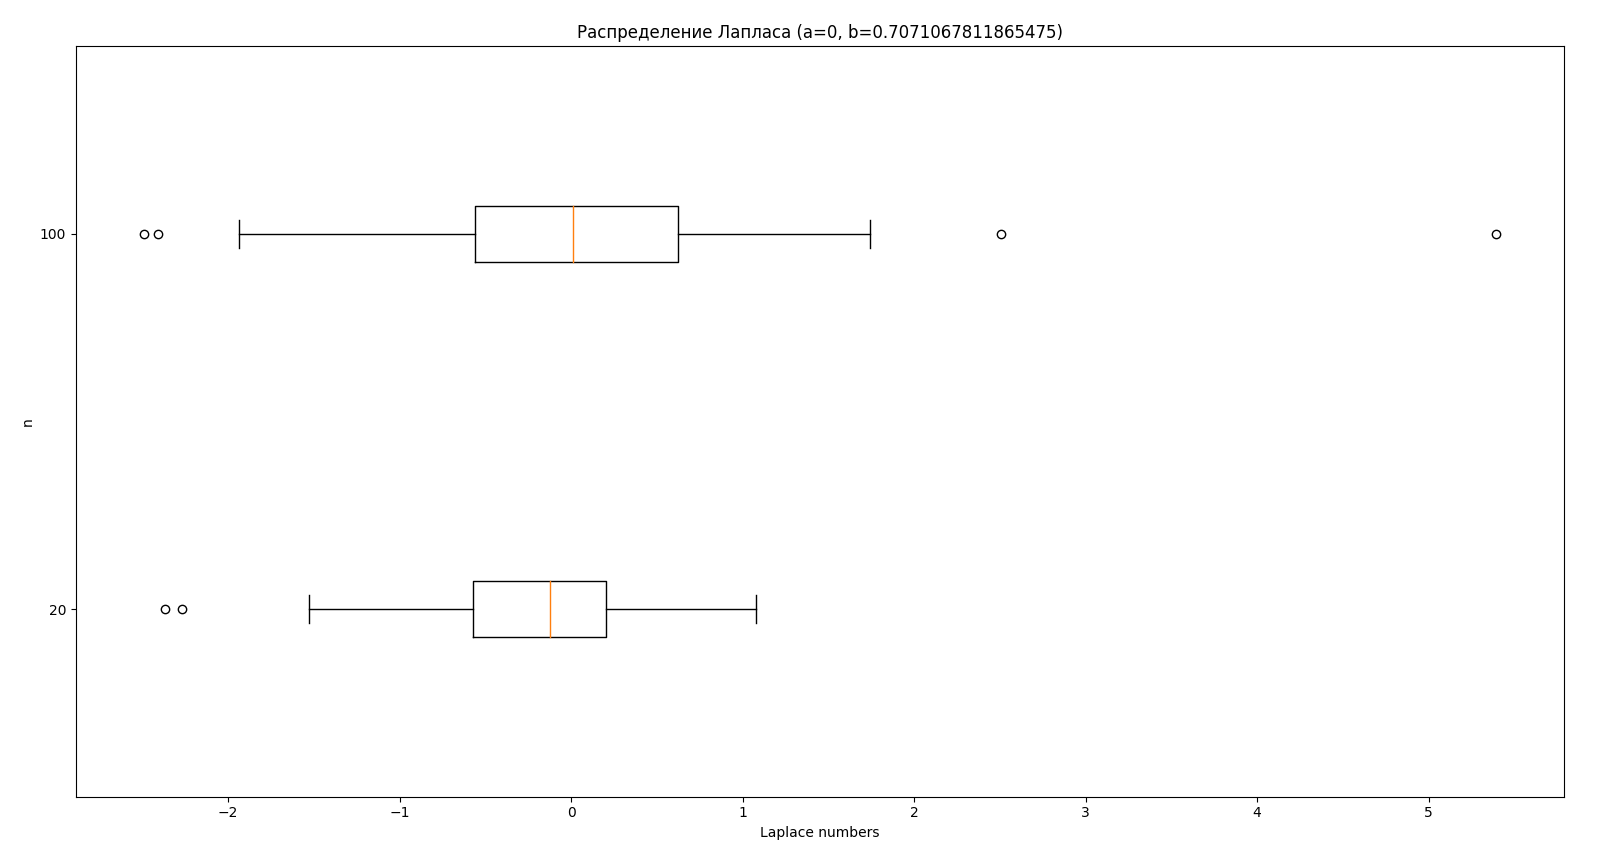
\includegraphics[scale=0.3]{resources/3_laplace.png}
	\caption{Боксплот распределения Лапласа}
\end{figure}

\begin{figure}[H]
	\centering
	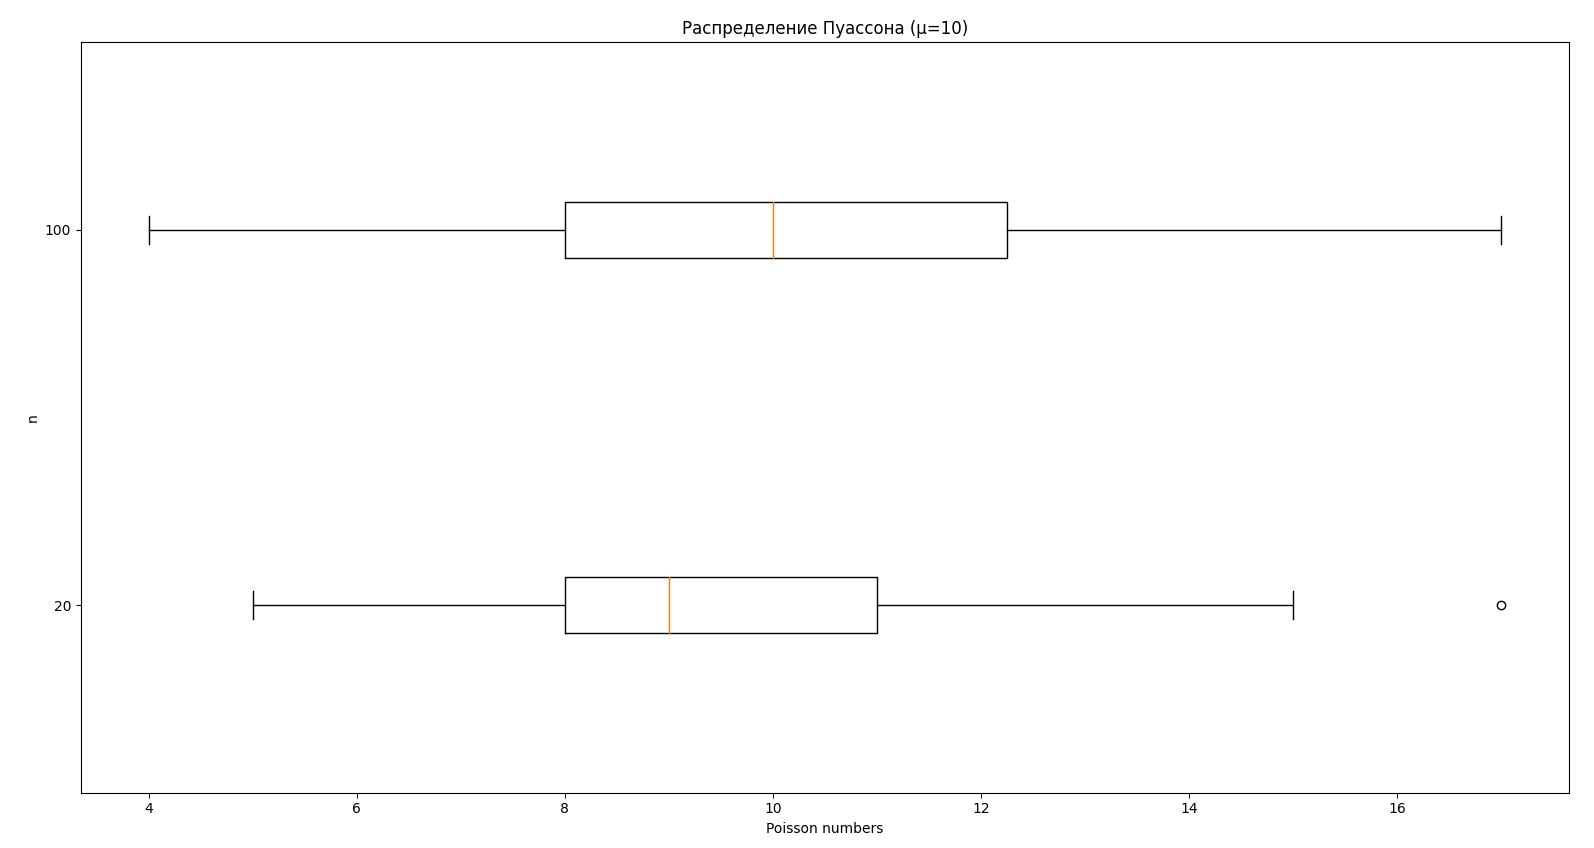
\includegraphics[scale=0.3]{resources/3_poisson.png}
	\caption{Боксплот распределения Пуассона}
\end{figure}

\begin{figure}[H]
	\centering
	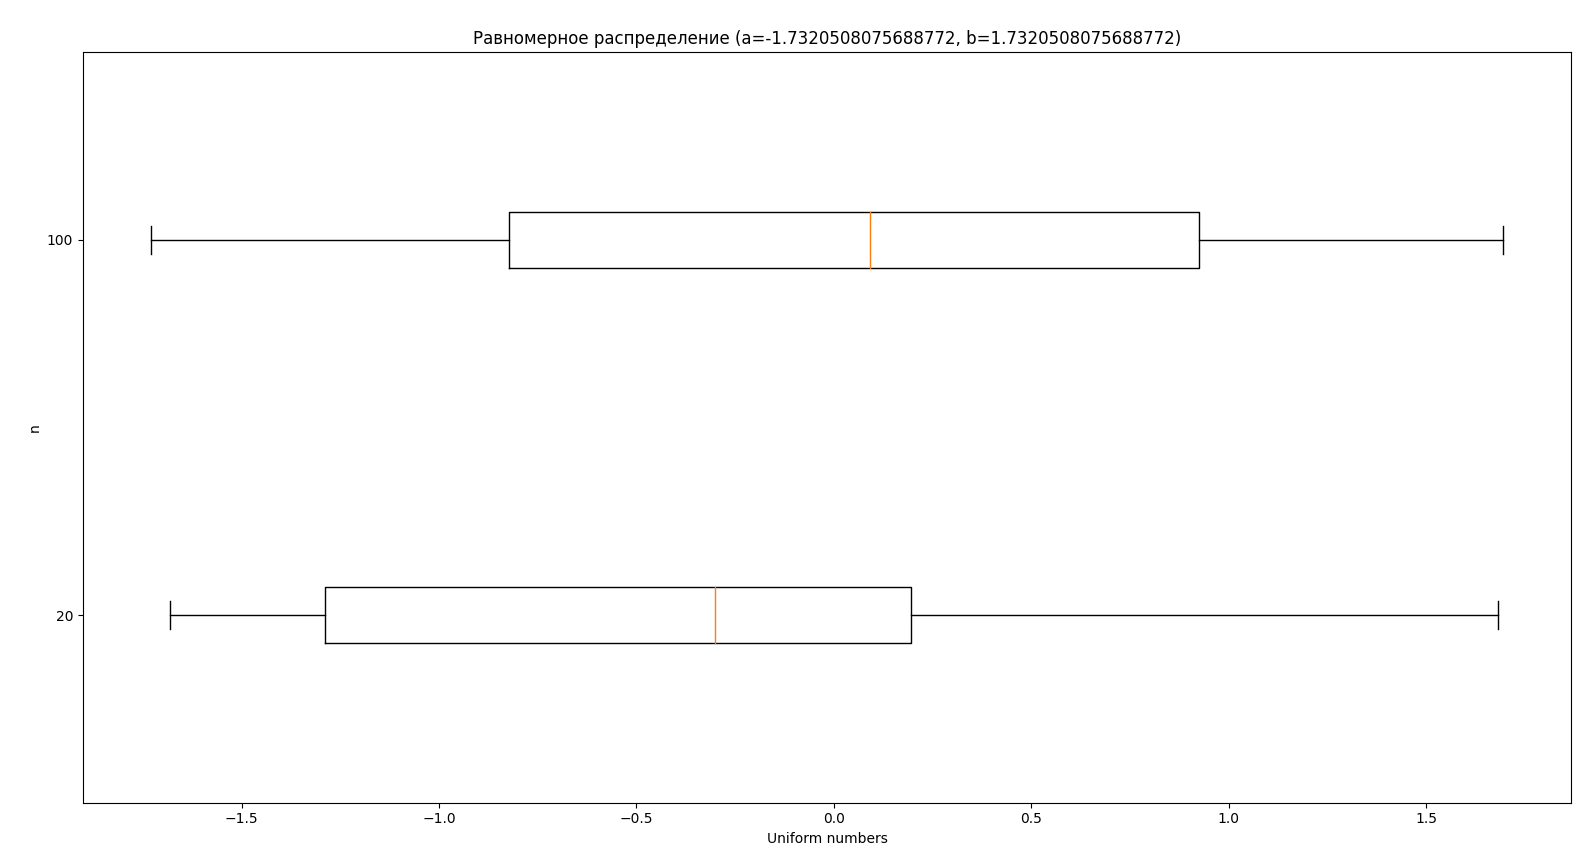
\includegraphics[scale=0.3]{resources/3_uniform.png}
	\caption{Боксплот равномерного распределения}
\end{figure}

\subsection{Доля выбросов}

\begin{table}[H]
	\begin{center}
		\begin{tabular}{|c|c|}
			\hline
			Выборка & Доля выбросов \\
			\hline\hline
			normal n=20 & 0.01\\
			\hline 
			normal n=100 & 0.02\\
			\hline
			cauchy n=20 & 0.16\\
			\hline 
			cauchy n=100 & 0.15\\
			\hline
			laplace n=20 & 0.07\\
			\hline 
			laplace n=100 & 0.07\\
			\hline
			poisson n=20 & 0.01\\
			\hline 
			poisson n=100 & 0.02\\
			\hline
			uniform n=20 & 0\\
			\hline 
			uniform n=100 & 0\\
			\hline
		\end{tabular}
	\end{center}
	\caption{Доля выбросов}
\end{table}

\subsection{Теоретическая вероятность выбросов}

\begin{table}[H]
	\begin{center}
		\begin{tabular}{|c|c|c|c|c|c|}
			\hline 
			Распределение & $Q_{1}^{T}$ & $Q_{3}^{T}$ & $X_{1}^{T}$ & $X_{2}^{T}$ & $P_{B}^{T}$ \\
			\hline\hline 
			Нормальное распределение & -0.674 & 0.674  & -2.698  & 2.698 & 0.007 \\
			\hline
			Распределение Коши & -1 & 1 &-4  &4 &0.156 \\
			\hline
			Распределение Лапласа & -0.490 & 0.490 &-1.961  &1.961 &0.063 \\
			\hline
			Распределение Пуассона & 8 & 12  & 2  & 18 & 0.008 \\
			\hline
			Равномерное распределение & -0.866 & 0.866  & -3.464  & 3.464 & 0 \\
			\hline
		\end{tabular}
	\end{center}
	\caption{Теоретическая вероятность выбросов}
\end{table}

\subsection{Эмпирическая функция распределения}

\begin{figure}[H]
	\begin{tabular}{ccc}
		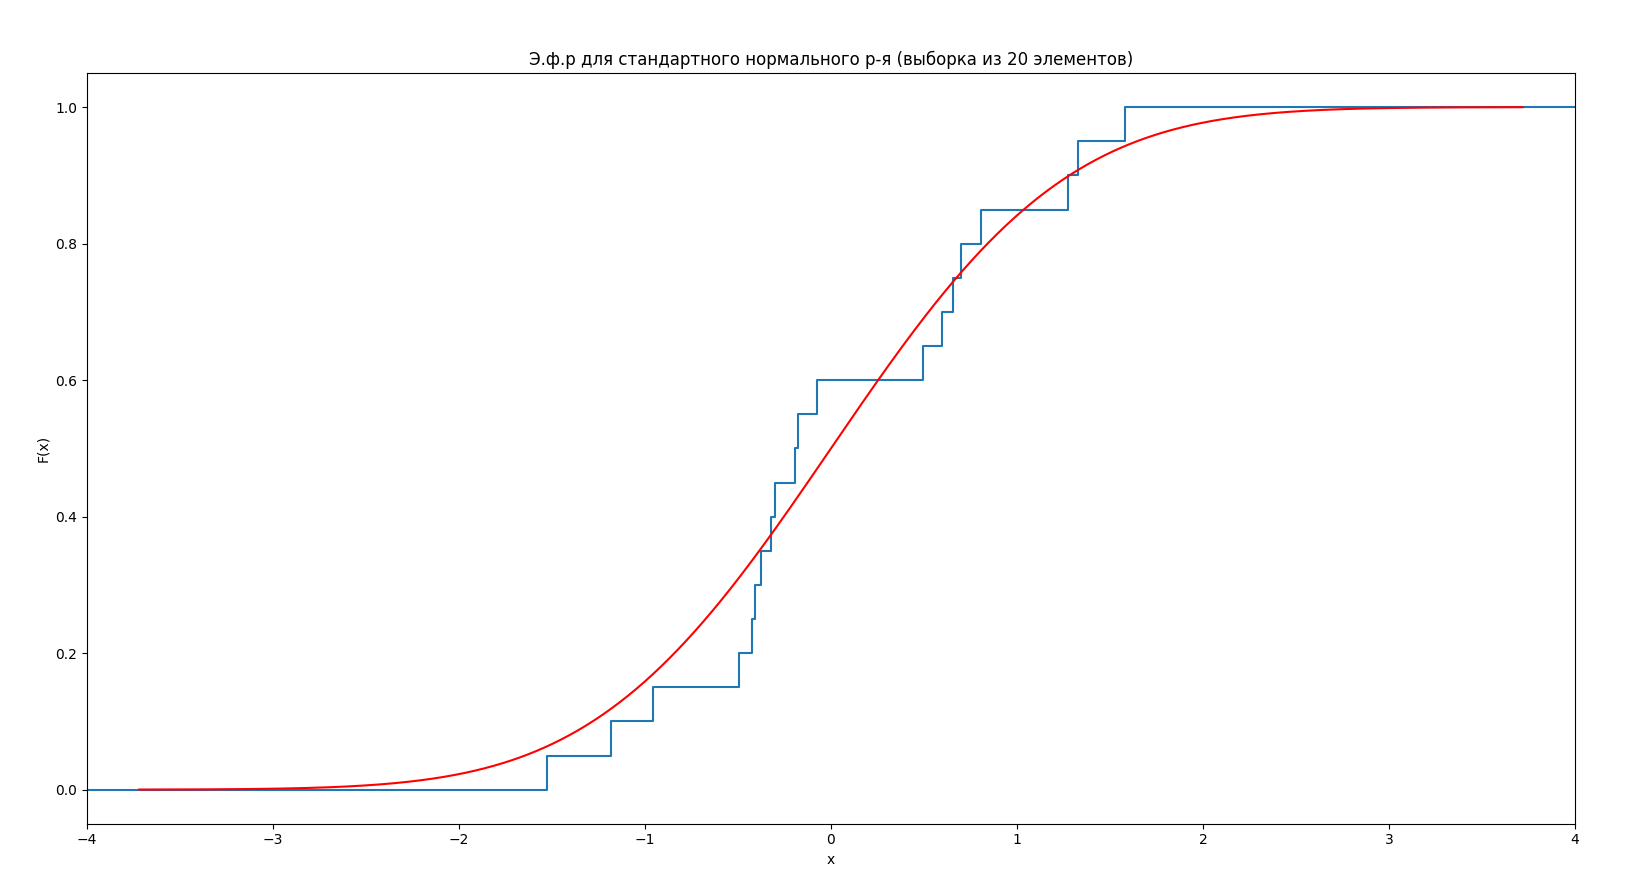
\includegraphics[scale=0.14]{resources/4_gauss_20.png}
		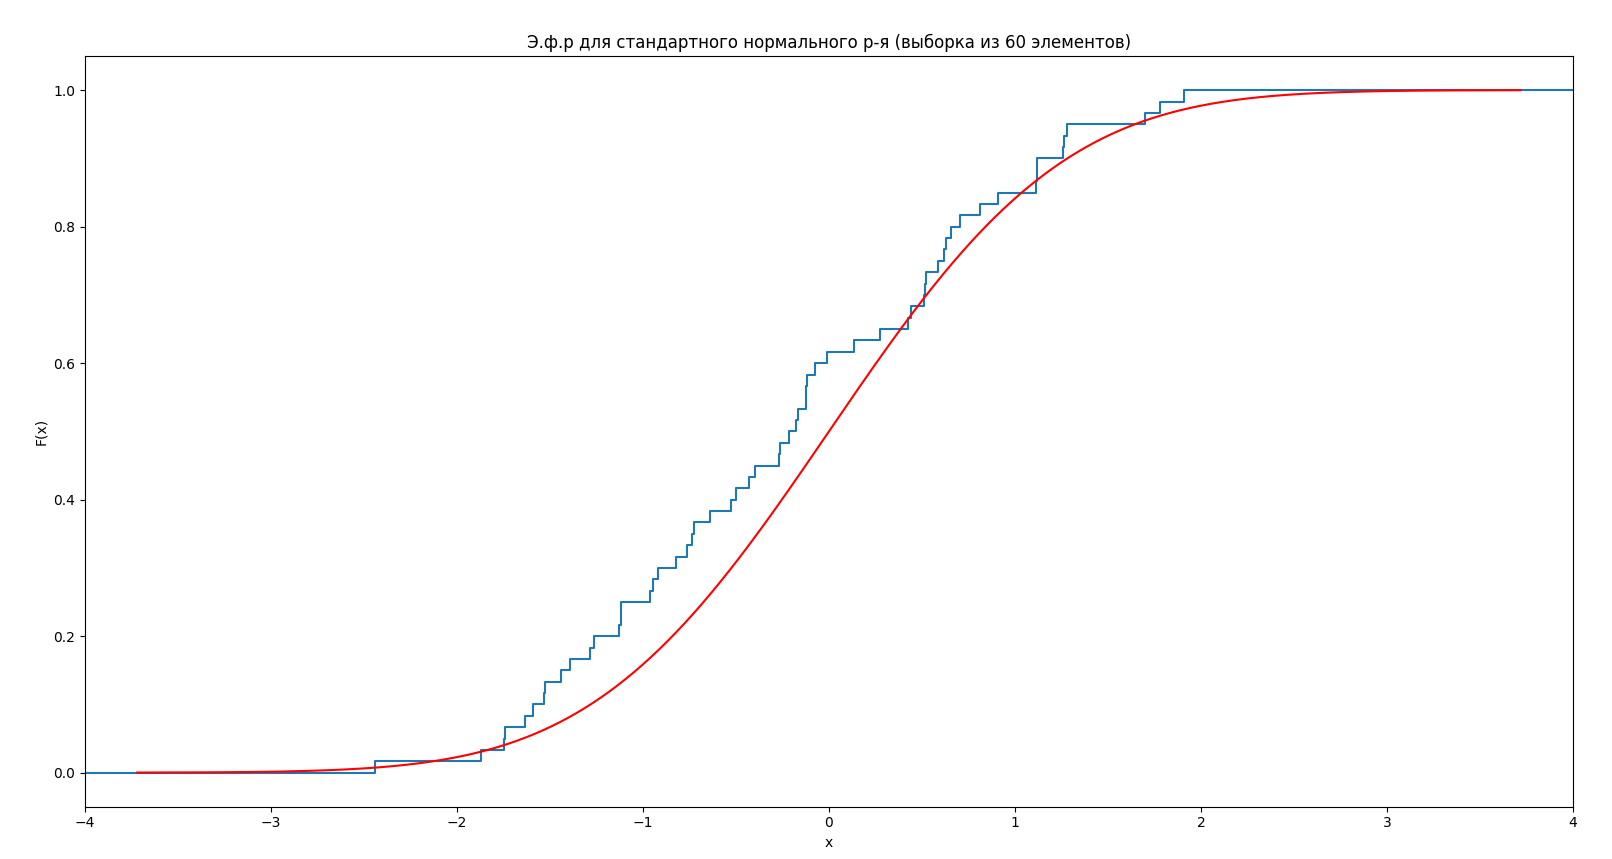
\includegraphics[scale=0.14]{resources/4_gauss_60.png}
		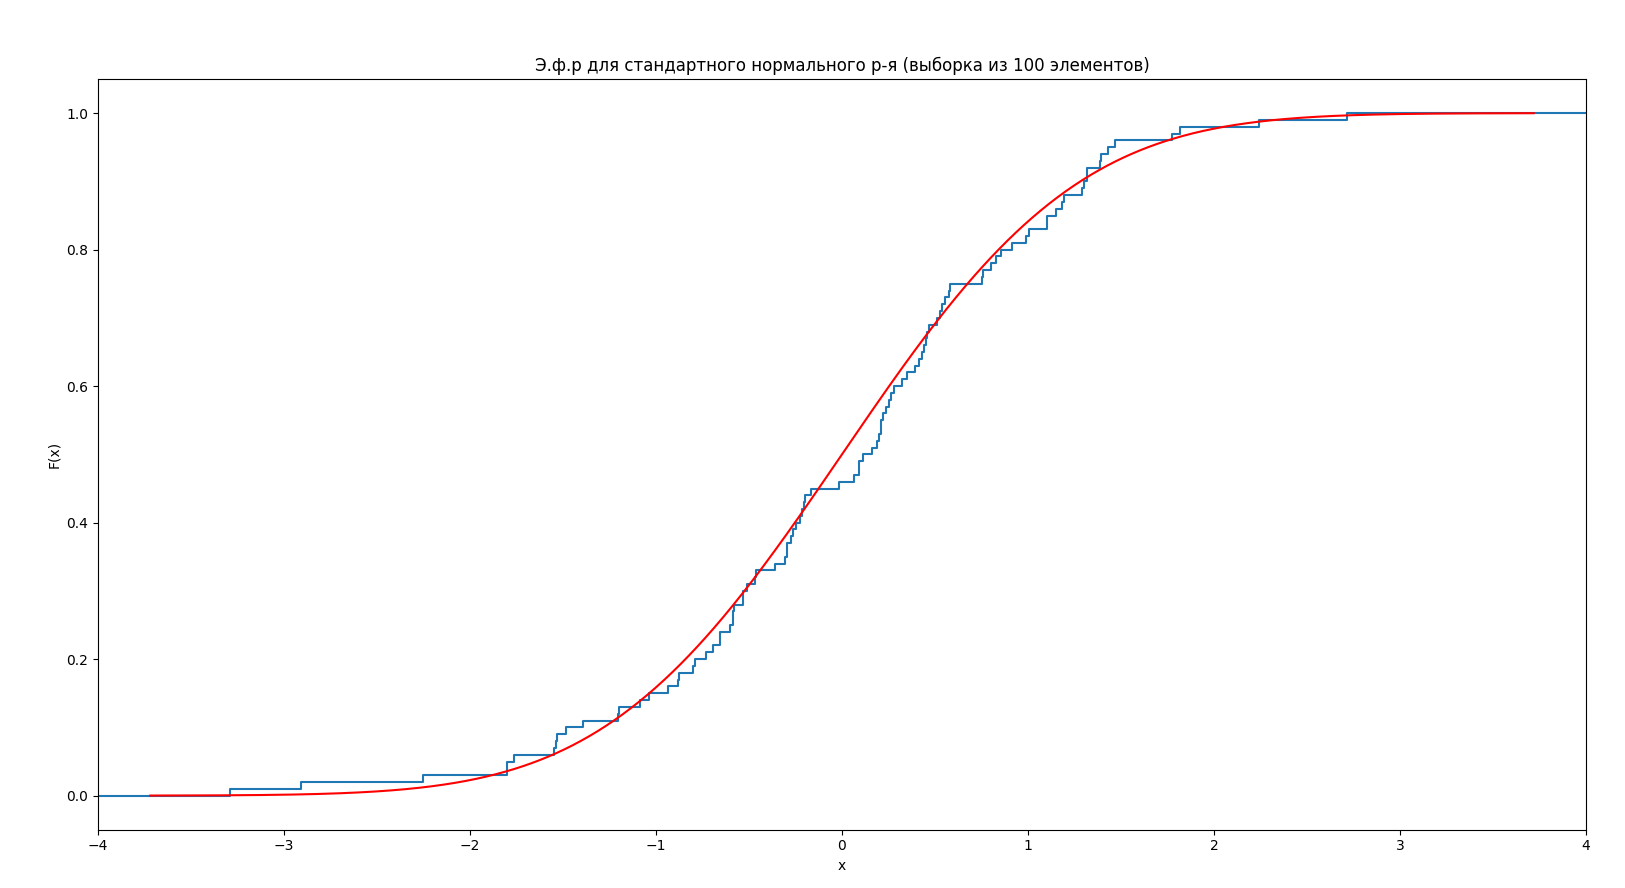
\includegraphics[scale=0.14]{resources/4_gauss_100.png}
	\end{tabular}
	\text{\tab \tab \tab n=20 \tab \tab \tab \tab \tab n=60 \tab \tab \tab \tab \tab n=100 \tab \tab }
	\caption{Нормальное распределение}
\end{figure}

\begin{figure}[H]
	\begin{tabular}{ccc}
		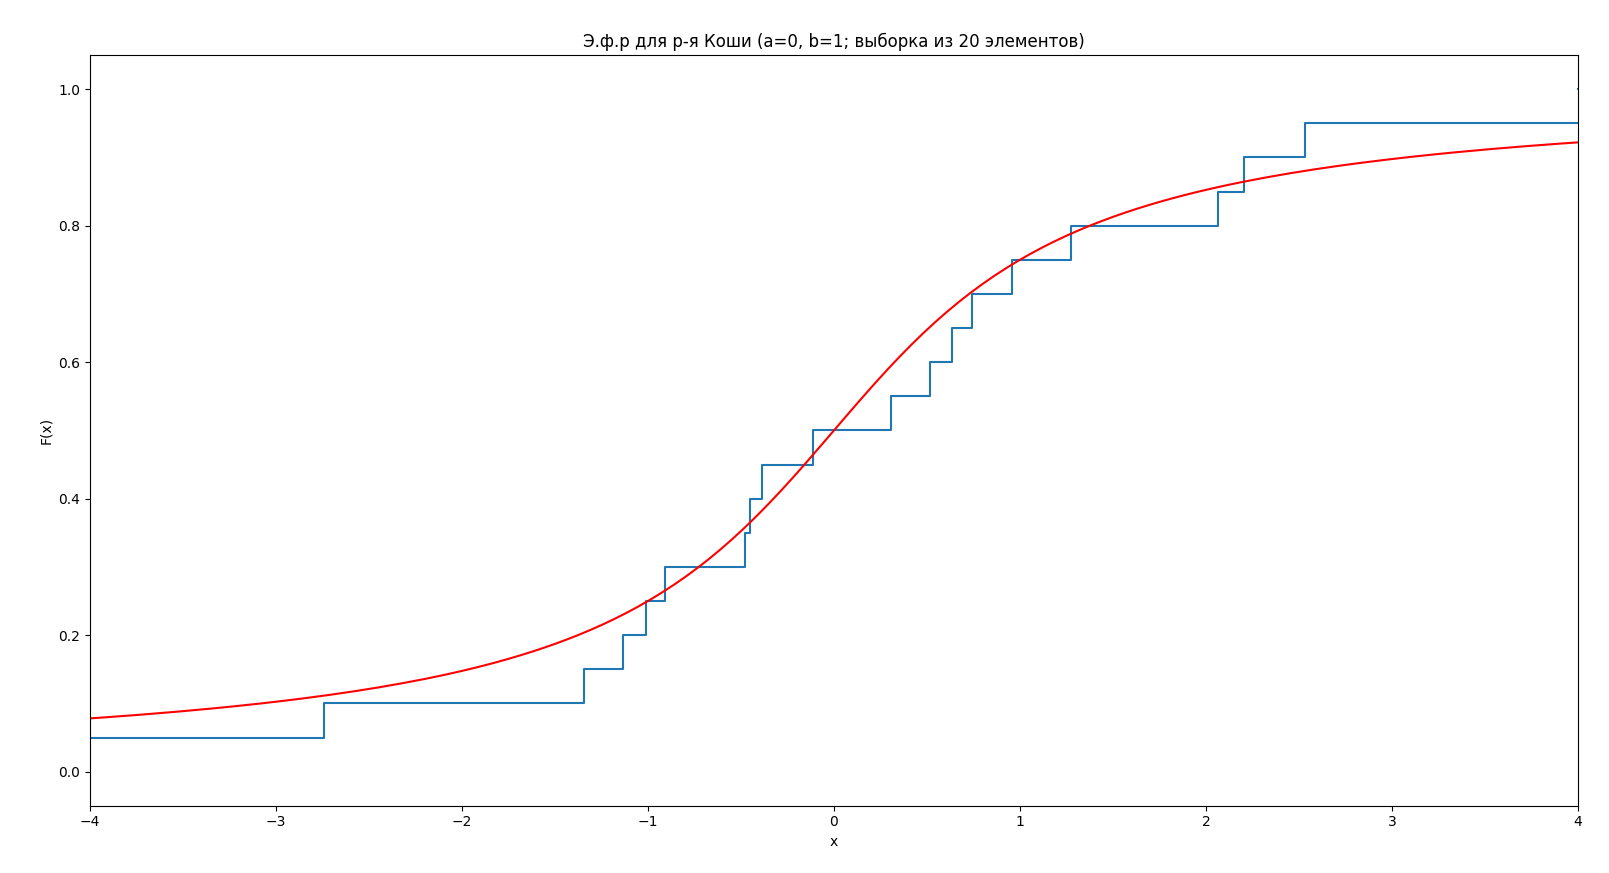
\includegraphics[scale=0.14]{resources/4_cauchy_20.png}
		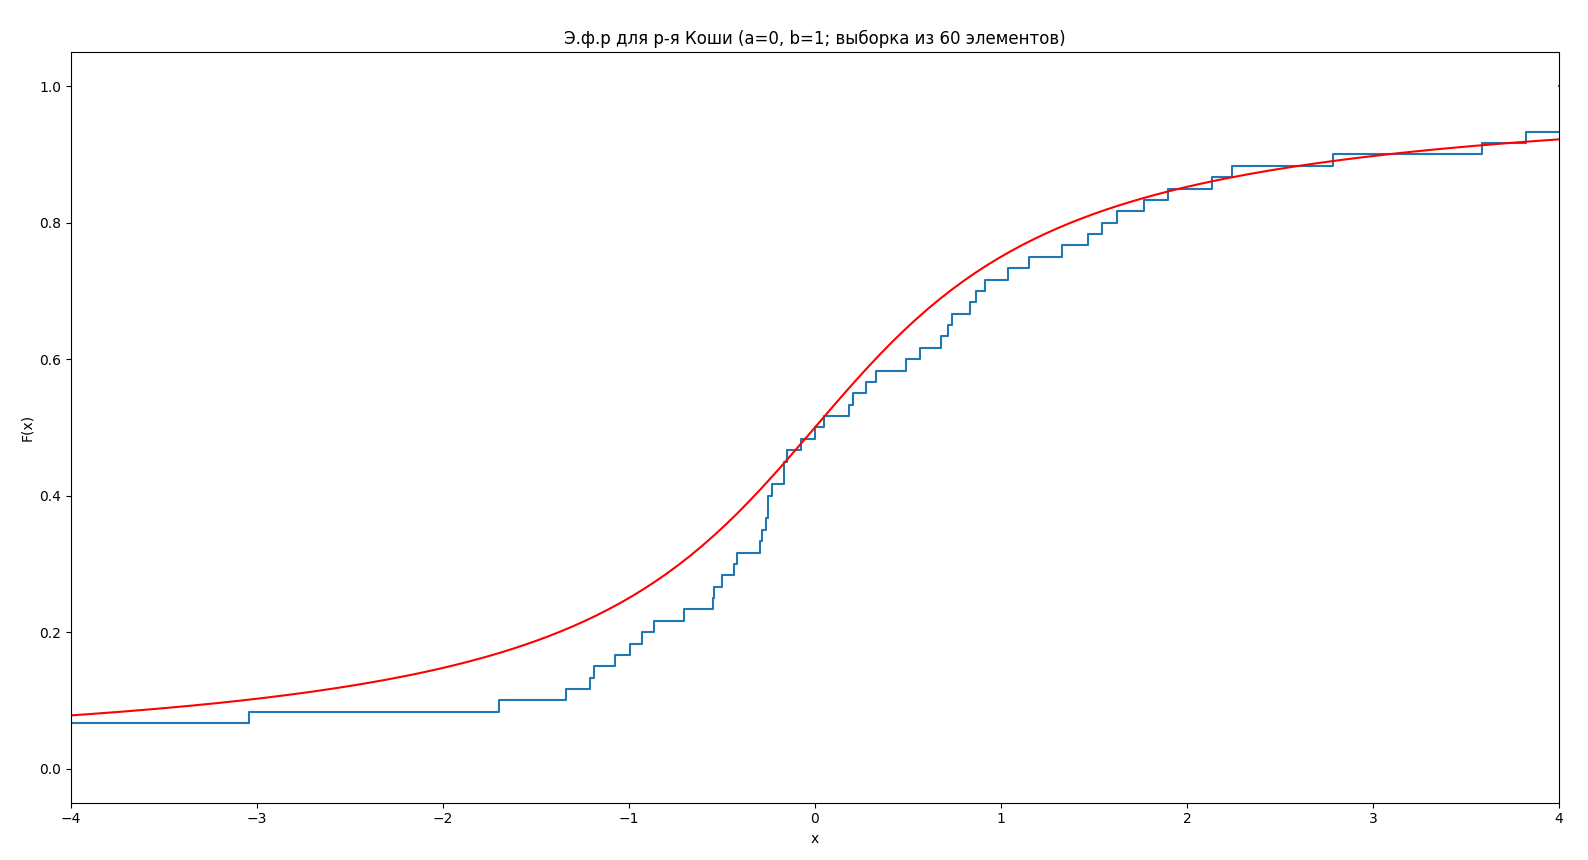
\includegraphics[scale=0.14]{resources/4_cauchy_60.png}
		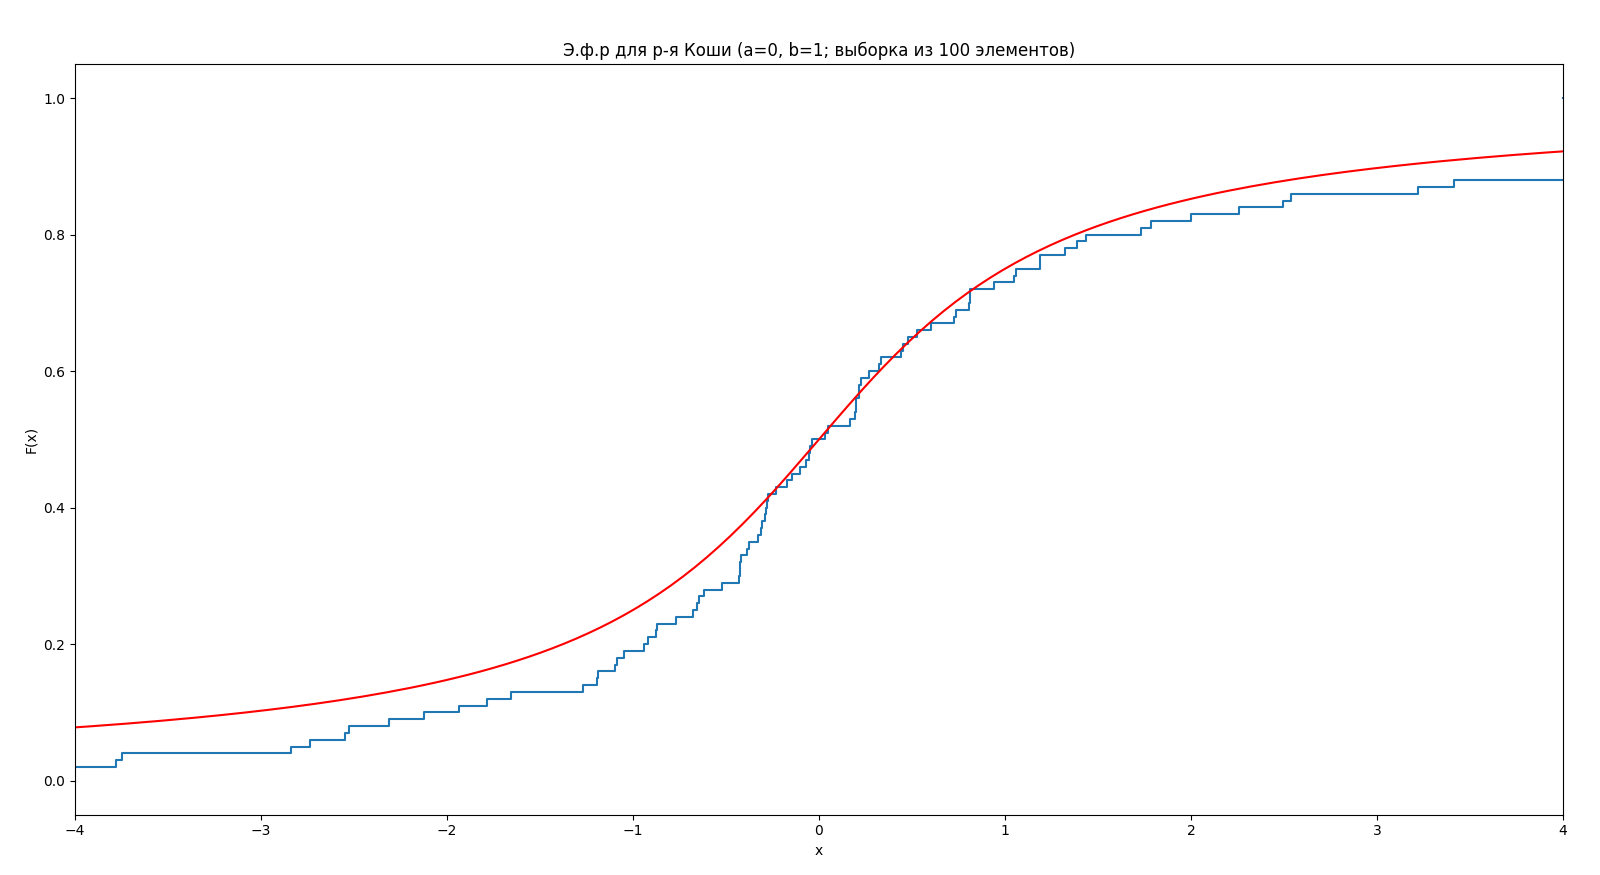
\includegraphics[scale=0.14]{resources/4_cauchy_100.png}
	\end{tabular}
	\text{\tab \tab \tab n=20 \tab \tab \tab \tab \tab n=60 \tab \tab \tab \tab \tab n=100 \tab \tab }
	\caption{Распределение Коши}
\end{figure}

\begin{figure}[H]
	\begin{tabular}{ccc}
		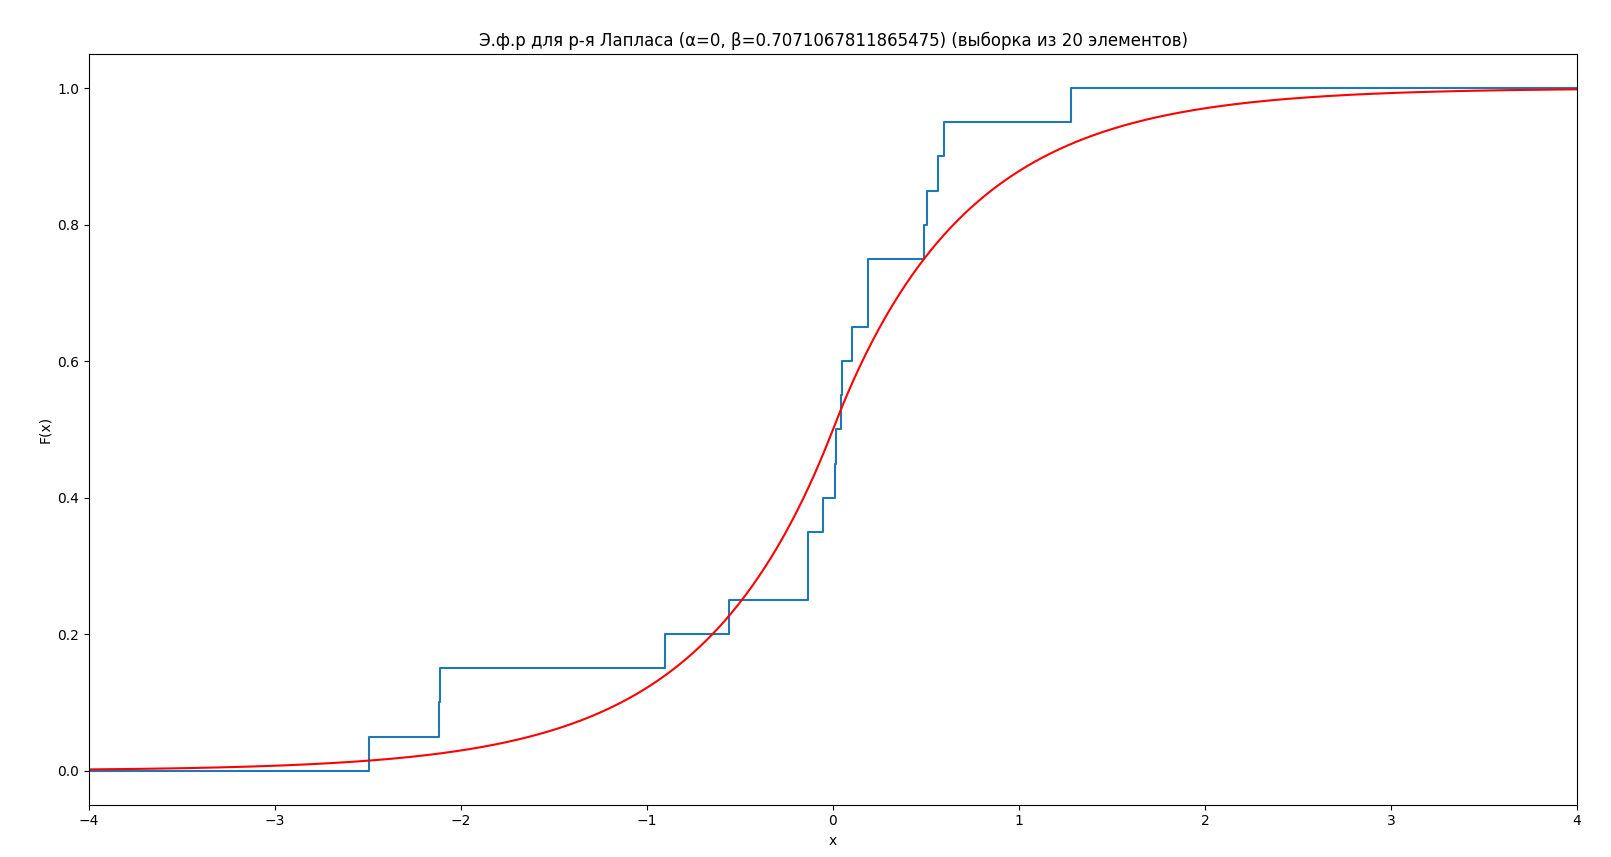
\includegraphics[scale=0.14]{resources/4_laplace_20.png}
		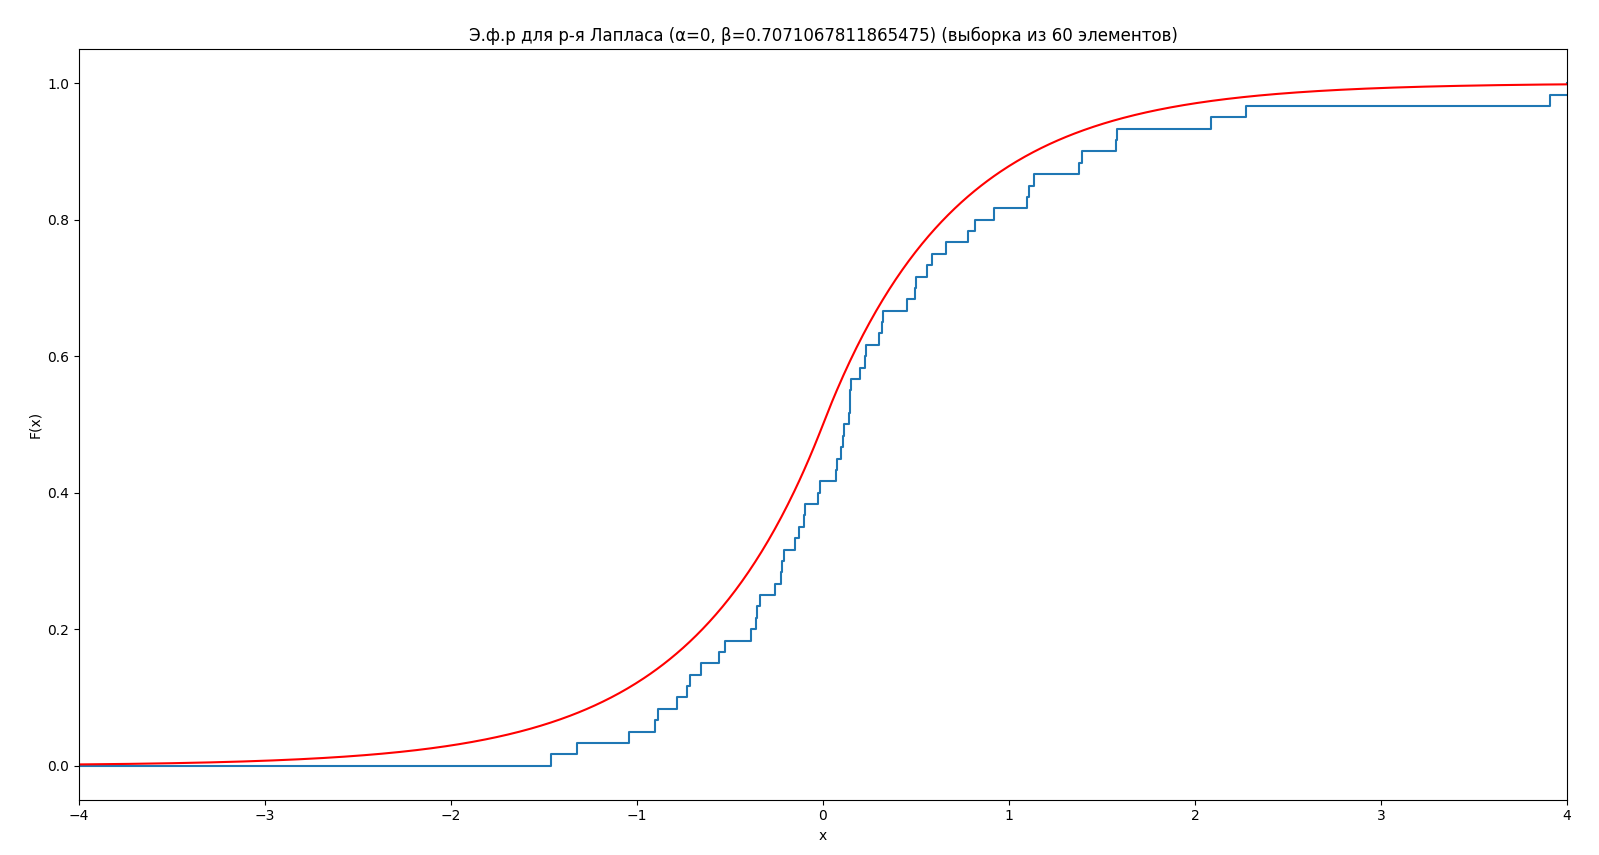
\includegraphics[scale=0.14]{resources/4_laplace_60.png}
		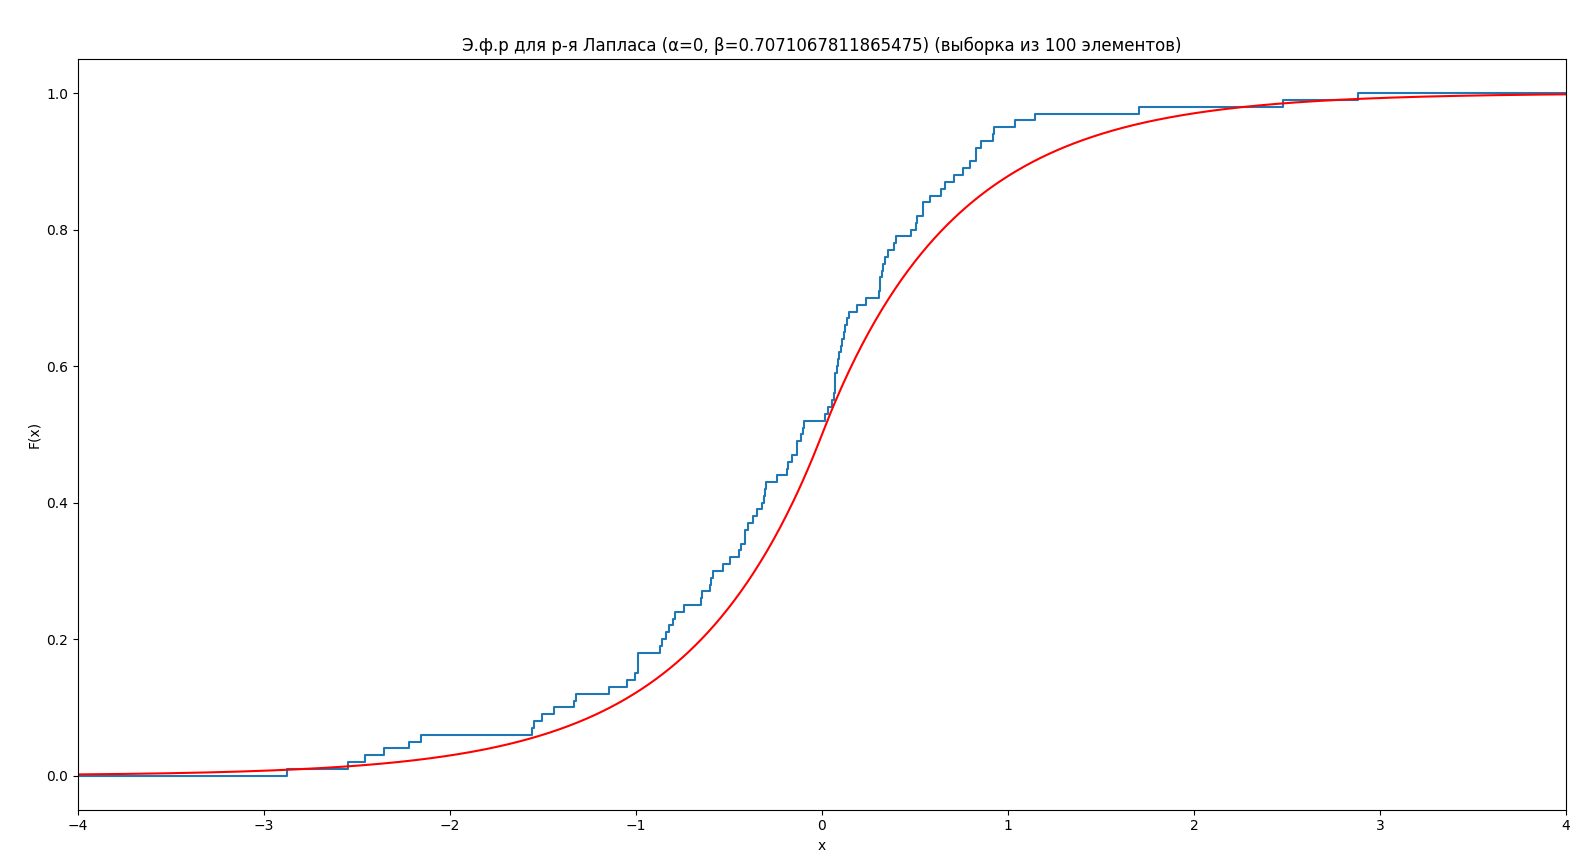
\includegraphics[scale=0.14]{resources/4_laplace_100.png}
	\end{tabular}
	\text{\tab \tab \tab n=20 \tab \tab \tab \tab \tab n=60 \tab \tab \tab \tab \tab n=100 \tab \tab }
	\caption{Распределение Лапласа}
\end{figure}

\begin{figure}[H]
	\begin{tabular}{ccc}
		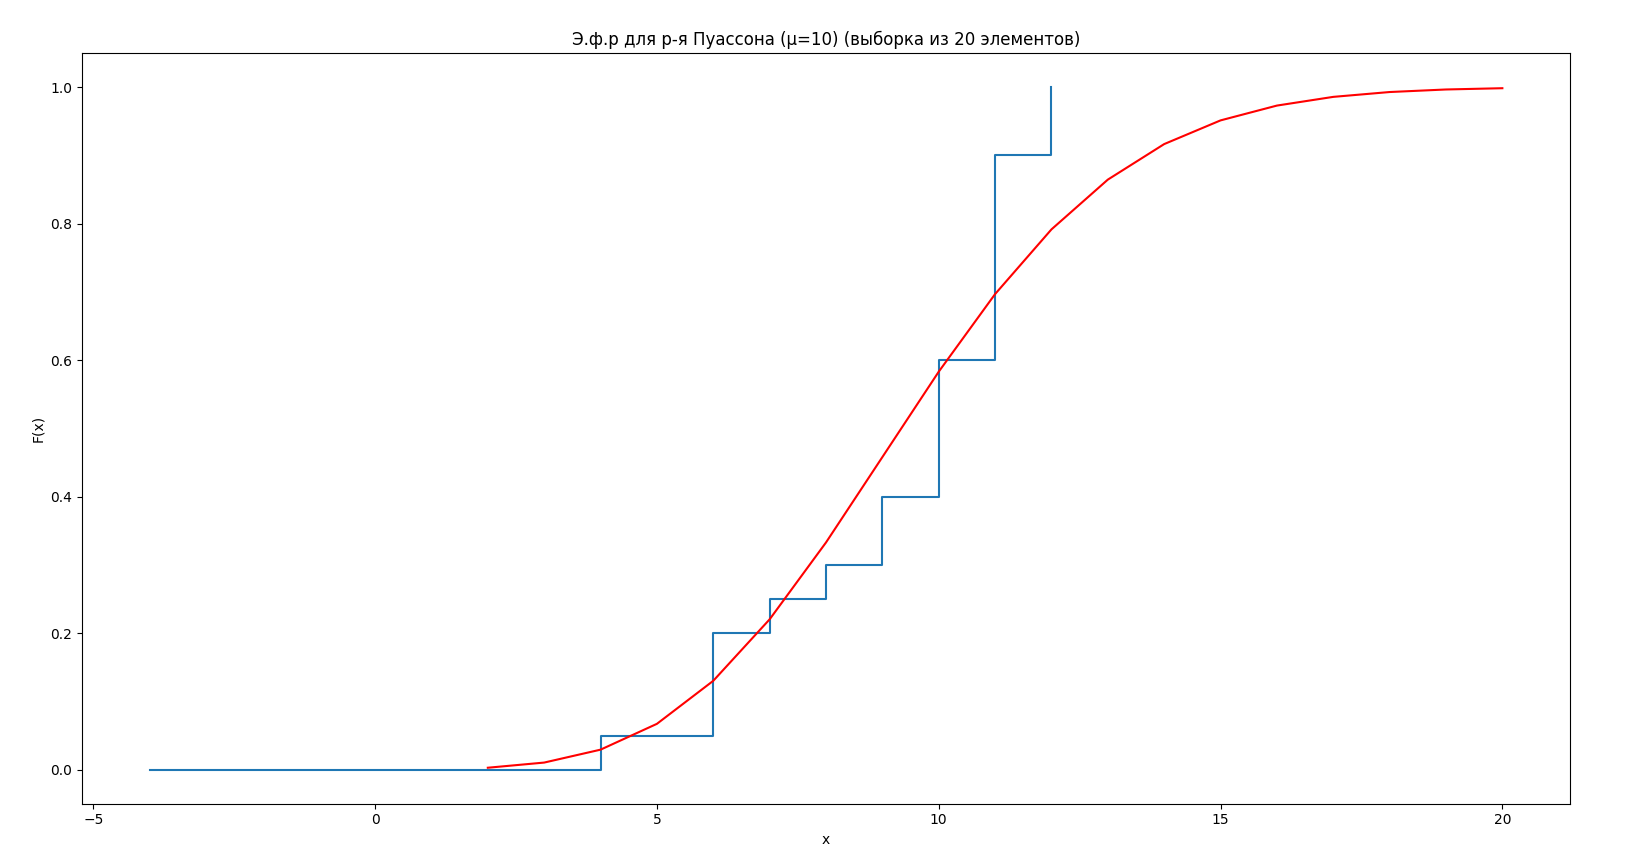
\includegraphics[scale=0.14]{resources/4_poisson_20.png}
		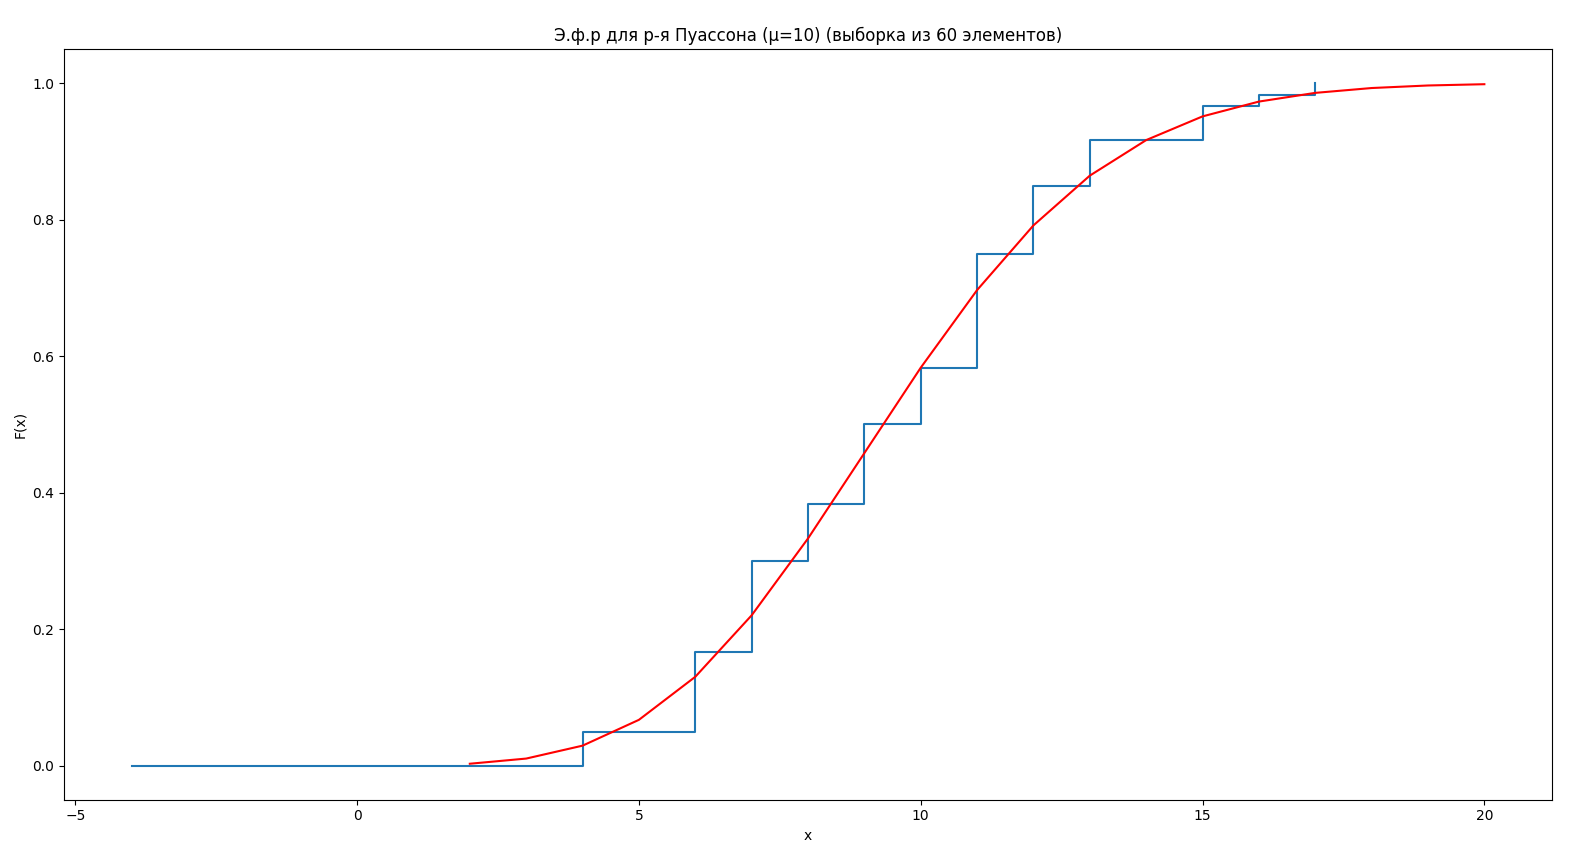
\includegraphics[scale=0.14]{resources/4_poisson_60.png}
		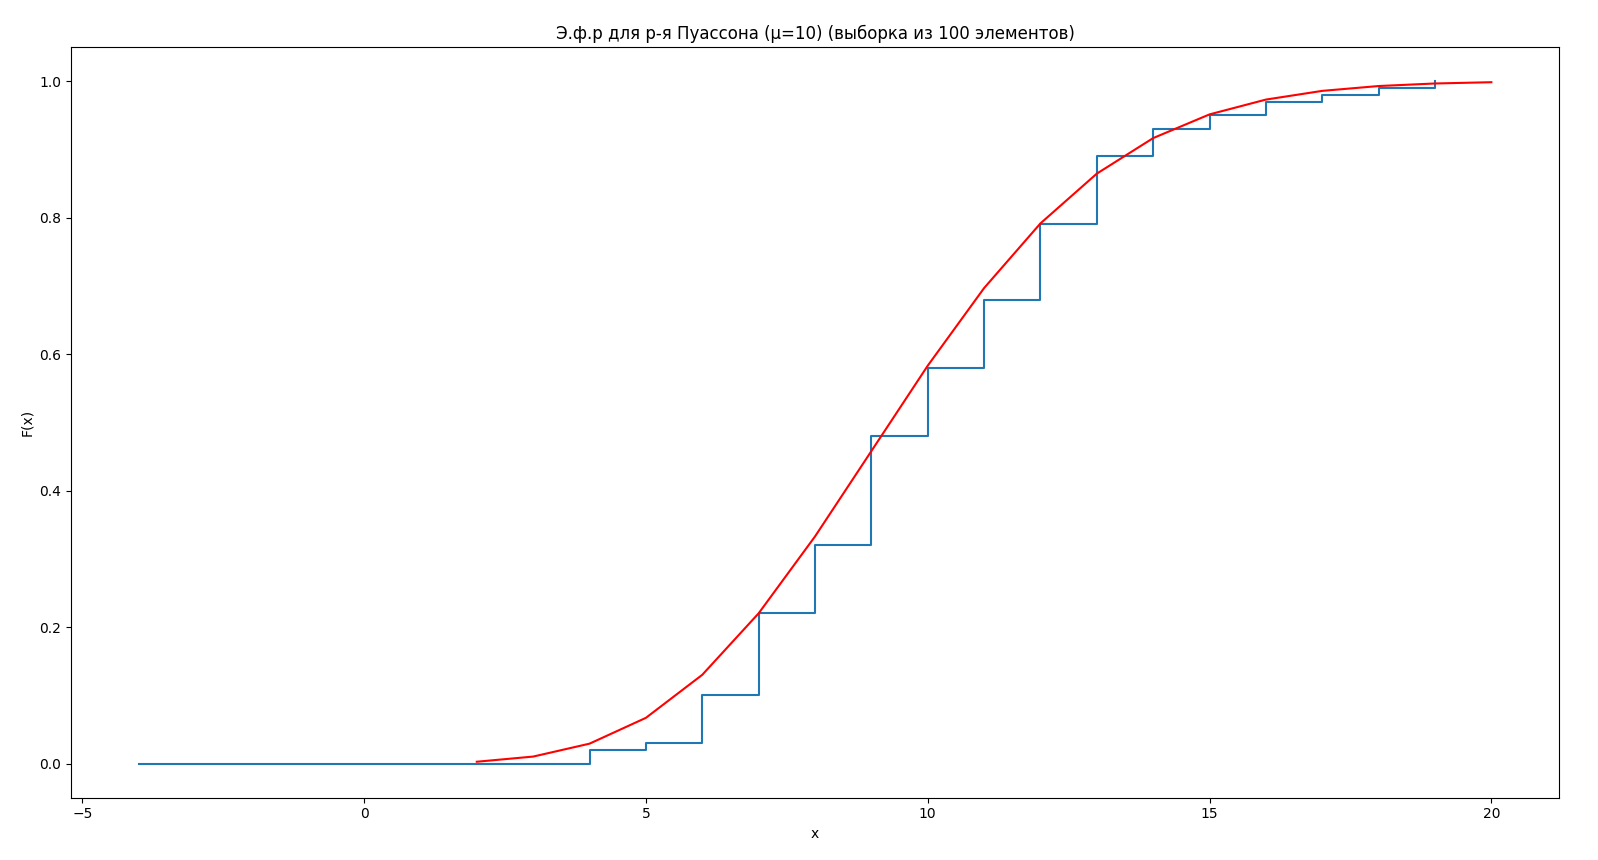
\includegraphics[scale=0.14]{resources/4_poisson_100.png}
	\end{tabular}
	\text{\tab \tab \tab n=20 \tab \tab \tab \tab \tab n=60 \tab \tab \tab \tab \tab n=100 \tab \tab }
	\caption{Распределение Пуассона}
\end{figure}


\begin{figure}[H]
	\begin{tabular}{ccc}
		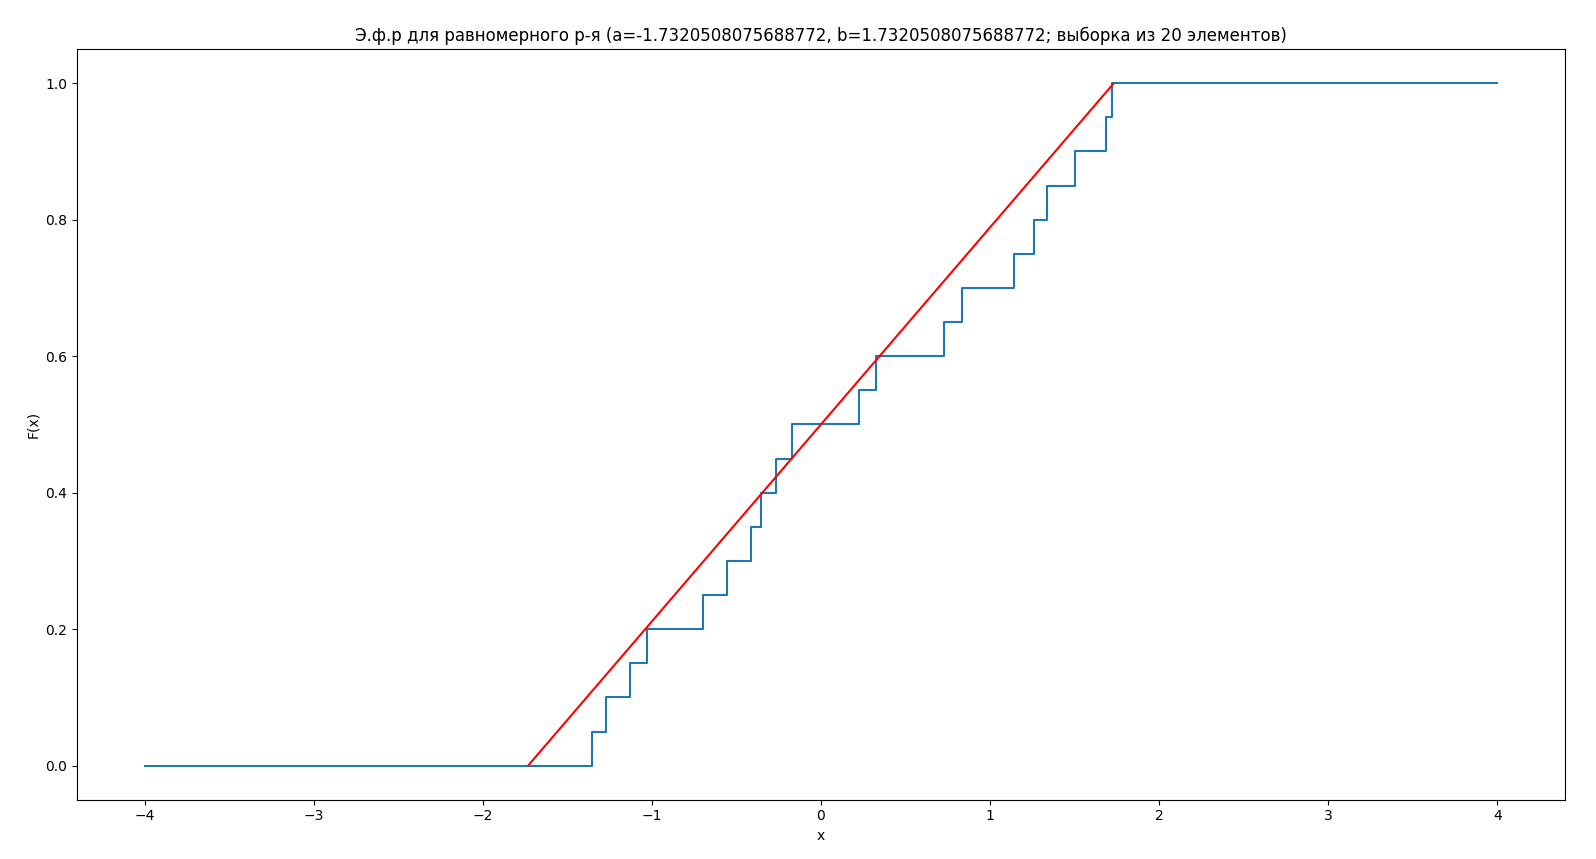
\includegraphics[scale=0.14]{resources/4_uniform_20.png}
		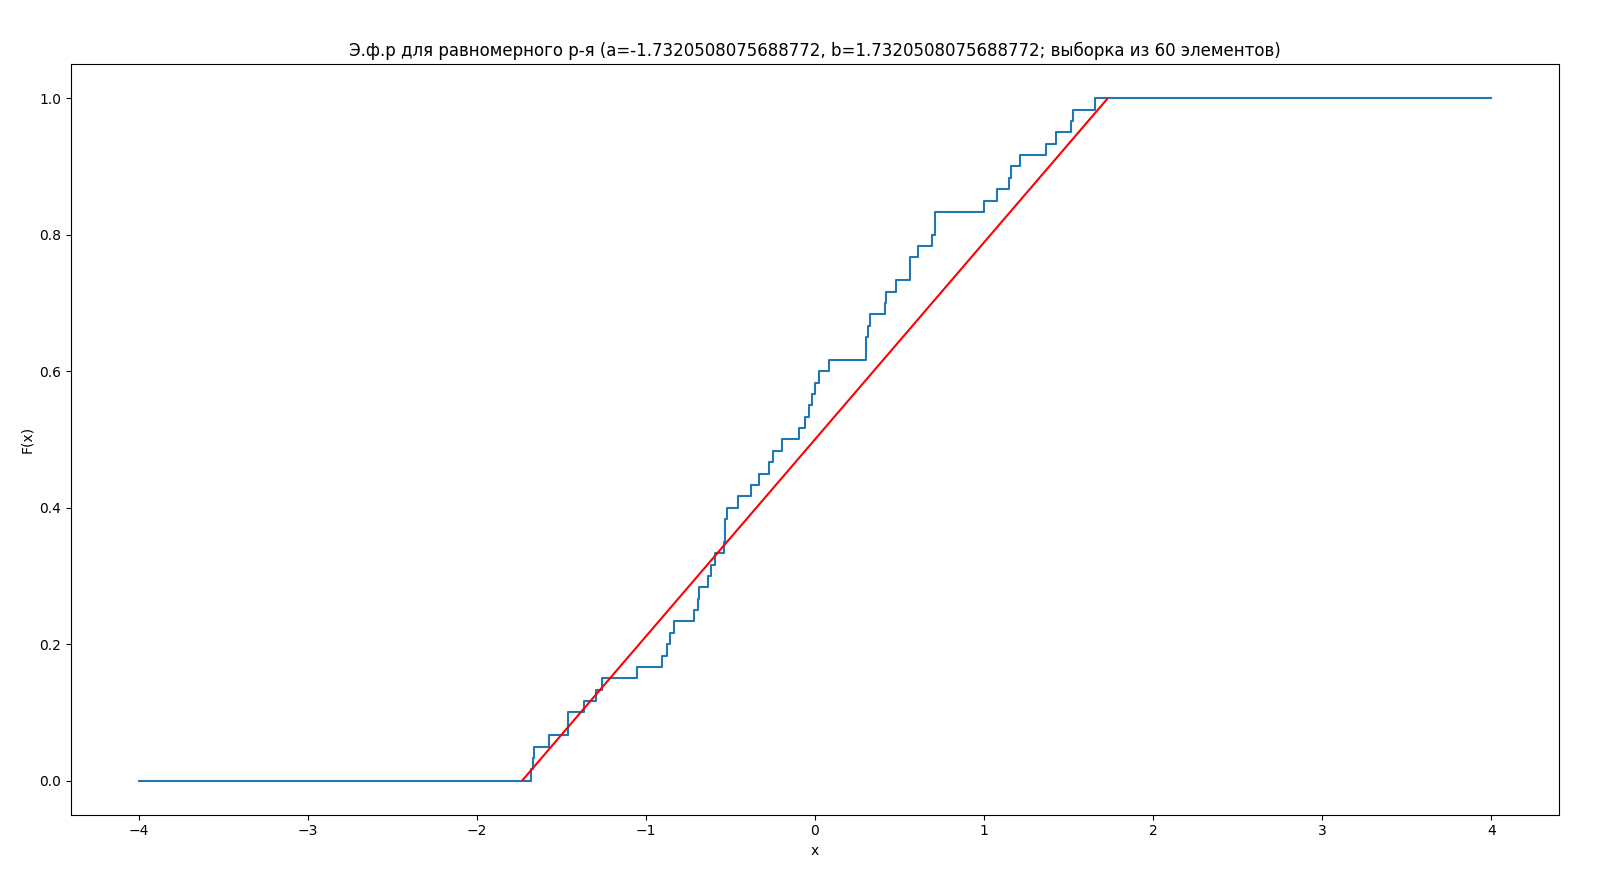
\includegraphics[scale=0.14]{resources/4_uniform_60.png}
		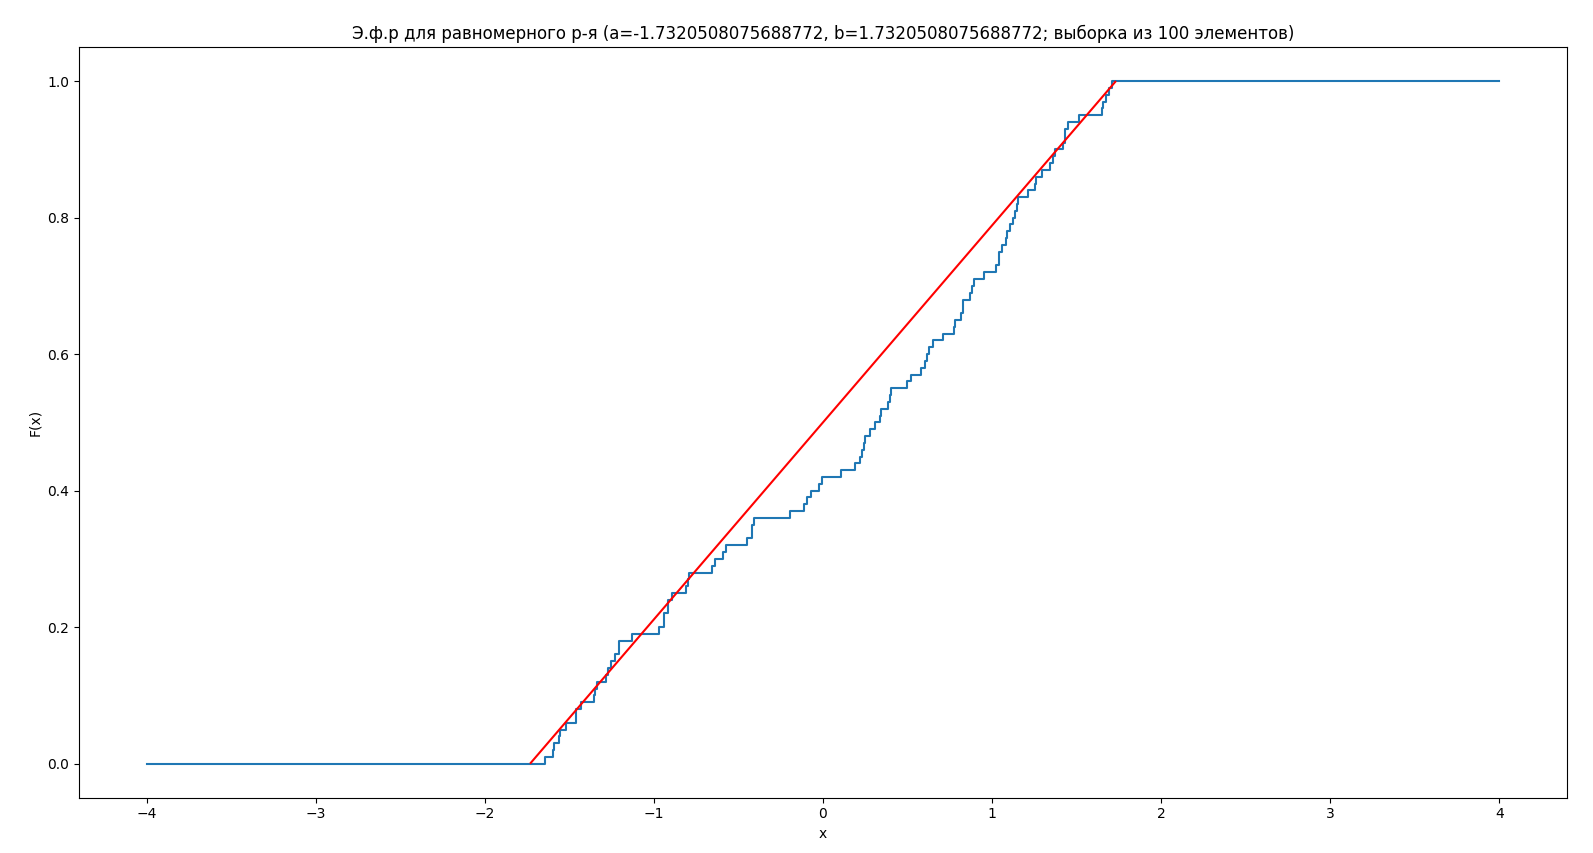
\includegraphics[scale=0.14]{resources/4_uniform_100.png}
	\end{tabular}
	\text{\tab \tab \tab n=20 \tab \tab \tab \tab \tab n=60 \tab \tab \tab \tab \tab n=100 \tab \tab }
	\caption{Равномерное распределение}
\end{figure}

\subsection{Ядерные оценки плотности распределения}

\begin{figure}[H]
	\begin{tabular}{ccc}
		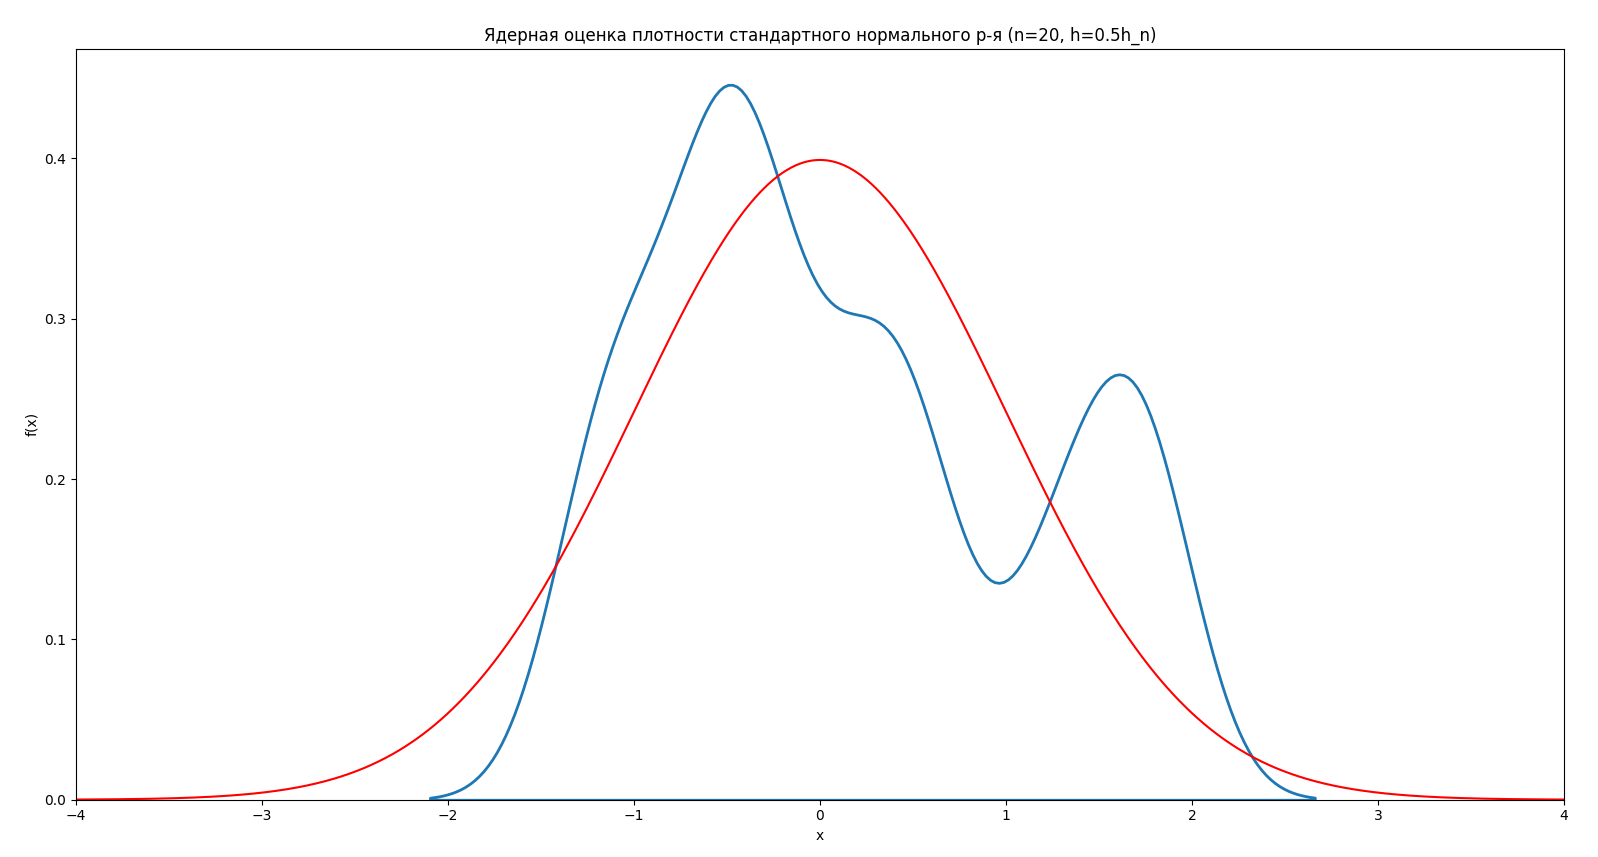
\includegraphics[scale=0.14]{resources/4_gauss_20_half.png}
		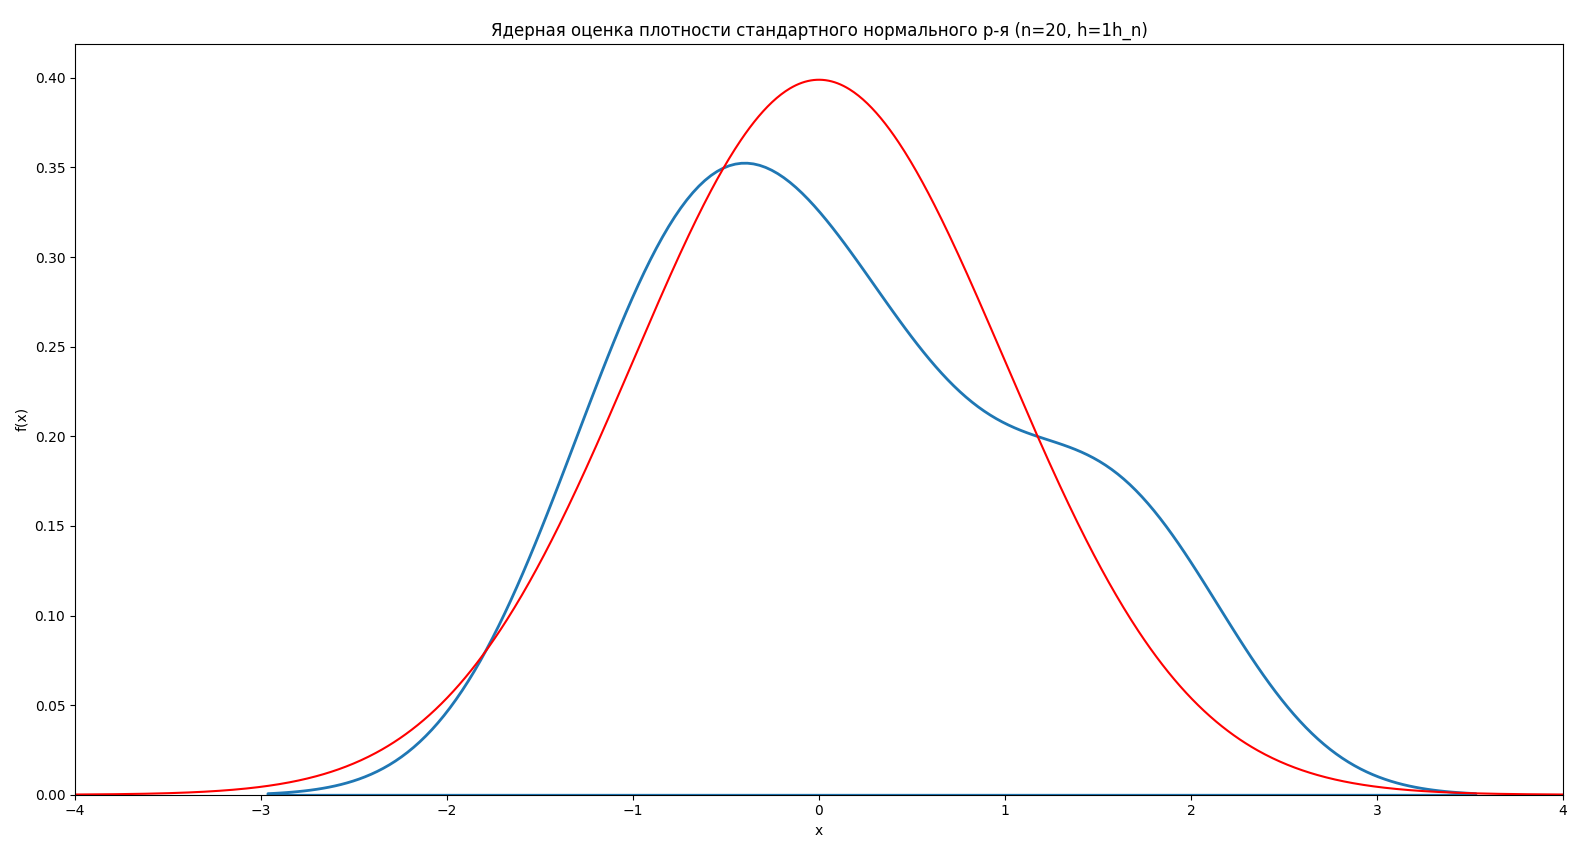
\includegraphics[scale=0.14]{resources/4_gauss_20_one.png}
		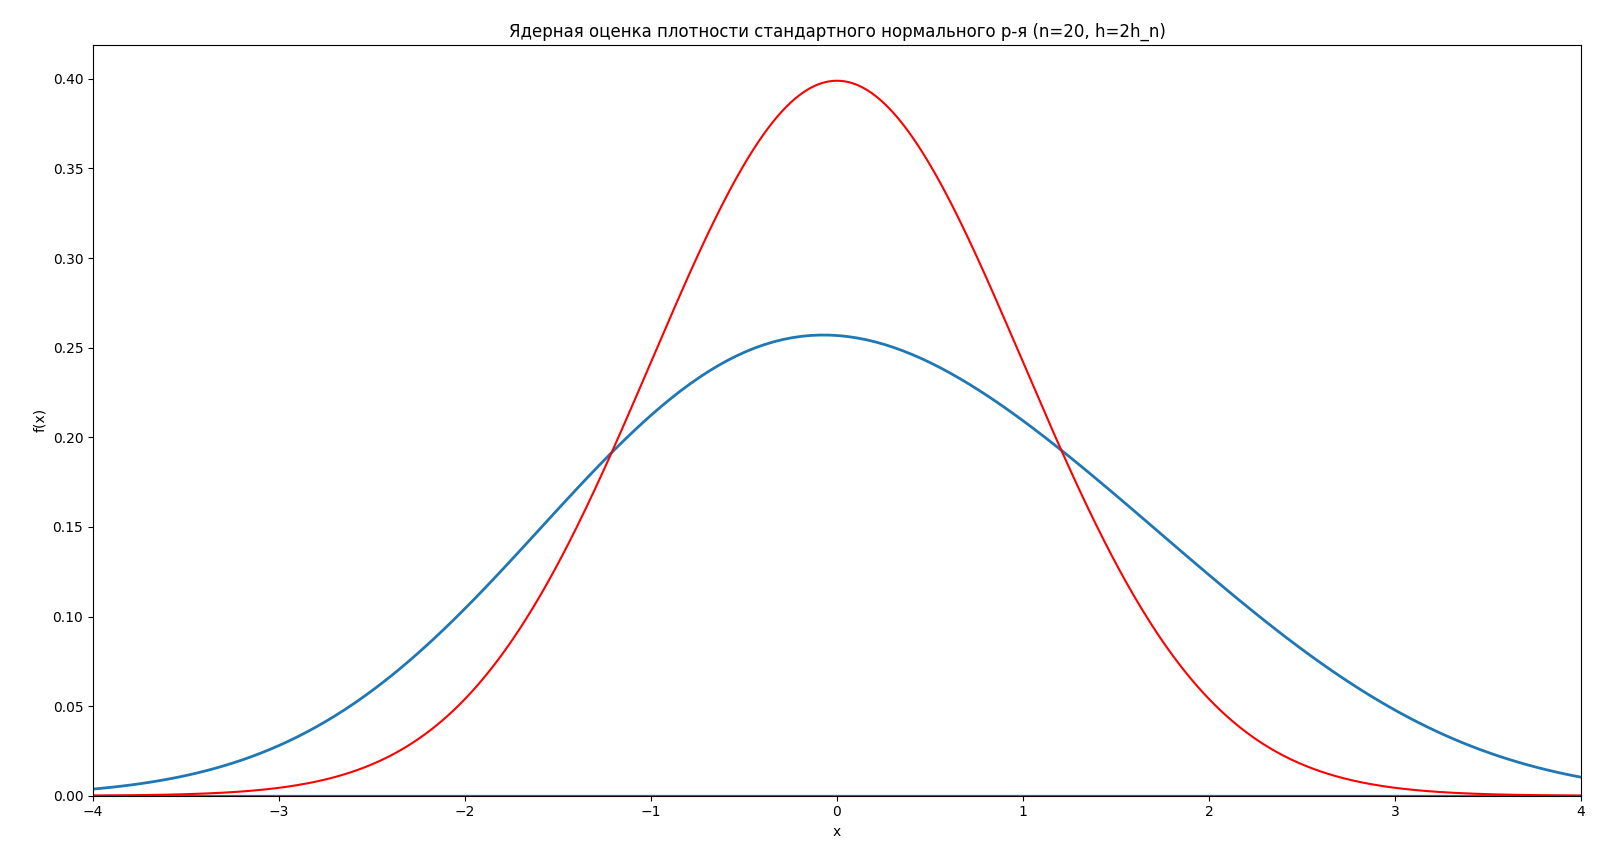
\includegraphics[scale=0.14]{resources/4_gauss_20_two.png}
	\end{tabular}
	\text{\tab \tab $h=h_{n}/2$ \tab \tab \tab \tab \tab $h=h_{n}$ \tab \tab \tab \tab \tab $h=2h_{n}$ \tab \tab }
	\caption{Нормальное распределение, $n=20$}
\end{figure}

\begin{figure}[H]
	\begin{tabular}{ccc}
		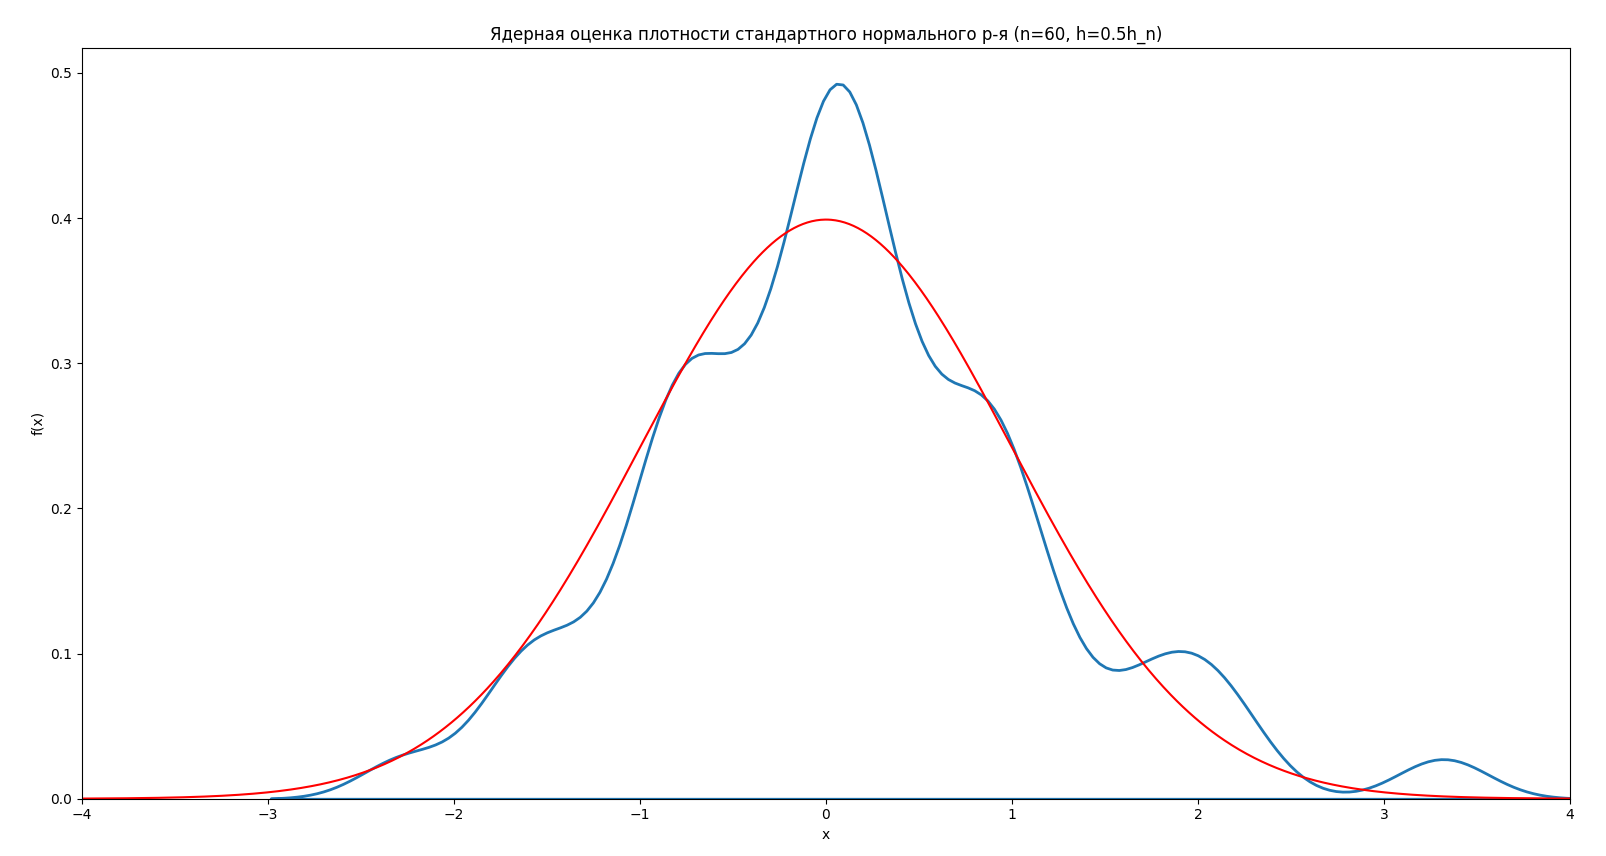
\includegraphics[scale=0.14]{resources/4_gauss_60_half.png}
		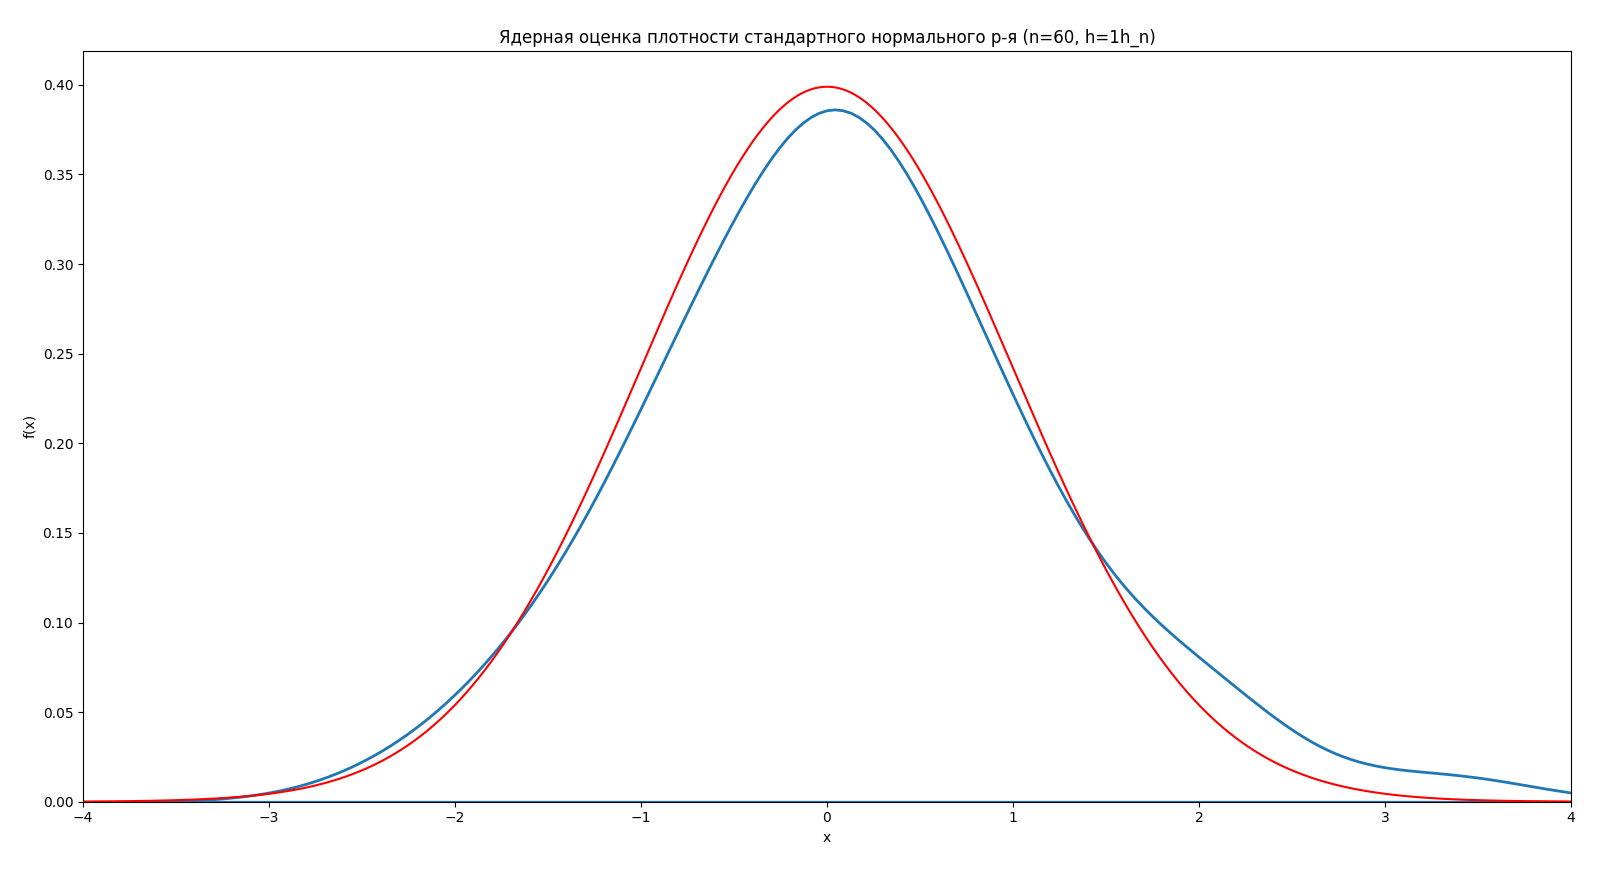
\includegraphics[scale=0.14]{resources/4_gauss_60_one.png}
		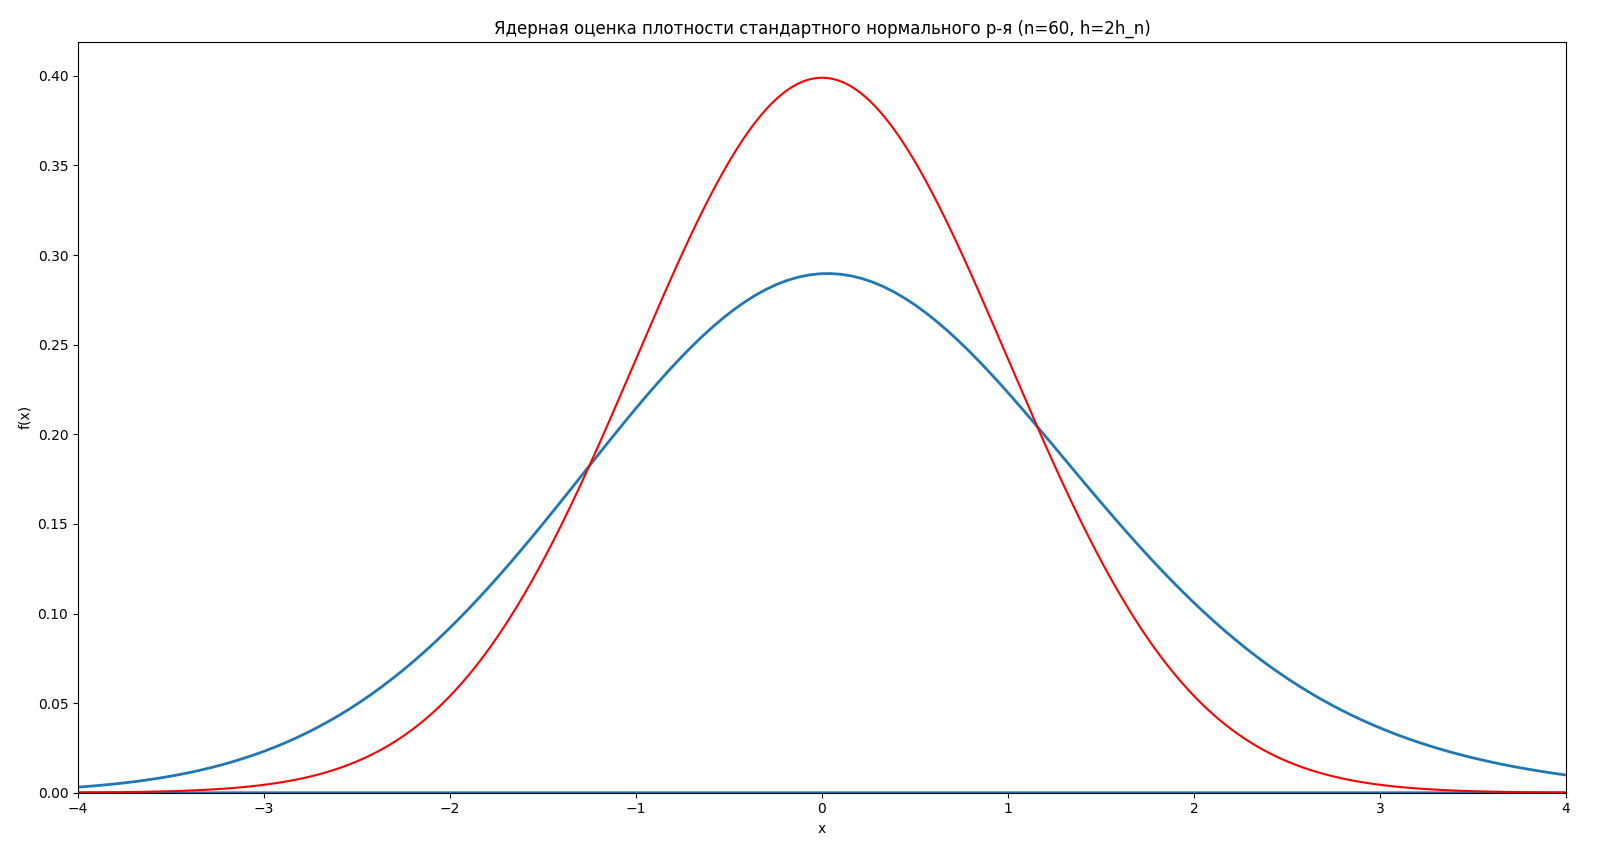
\includegraphics[scale=0.14]{resources/4_gauss_60_two.png}
	\end{tabular}
	\text{\tab \tab $h=h_{n}/2$ \tab \tab \tab \tab \tab $h=h_{n}$ \tab \tab \tab \tab \tab $h=2h_{n}$ \tab \tab }
	\caption{Нормальное распределение, $n=60$}
\end{figure}

\begin{figure}[H]
	\begin{tabular}{ccc}
		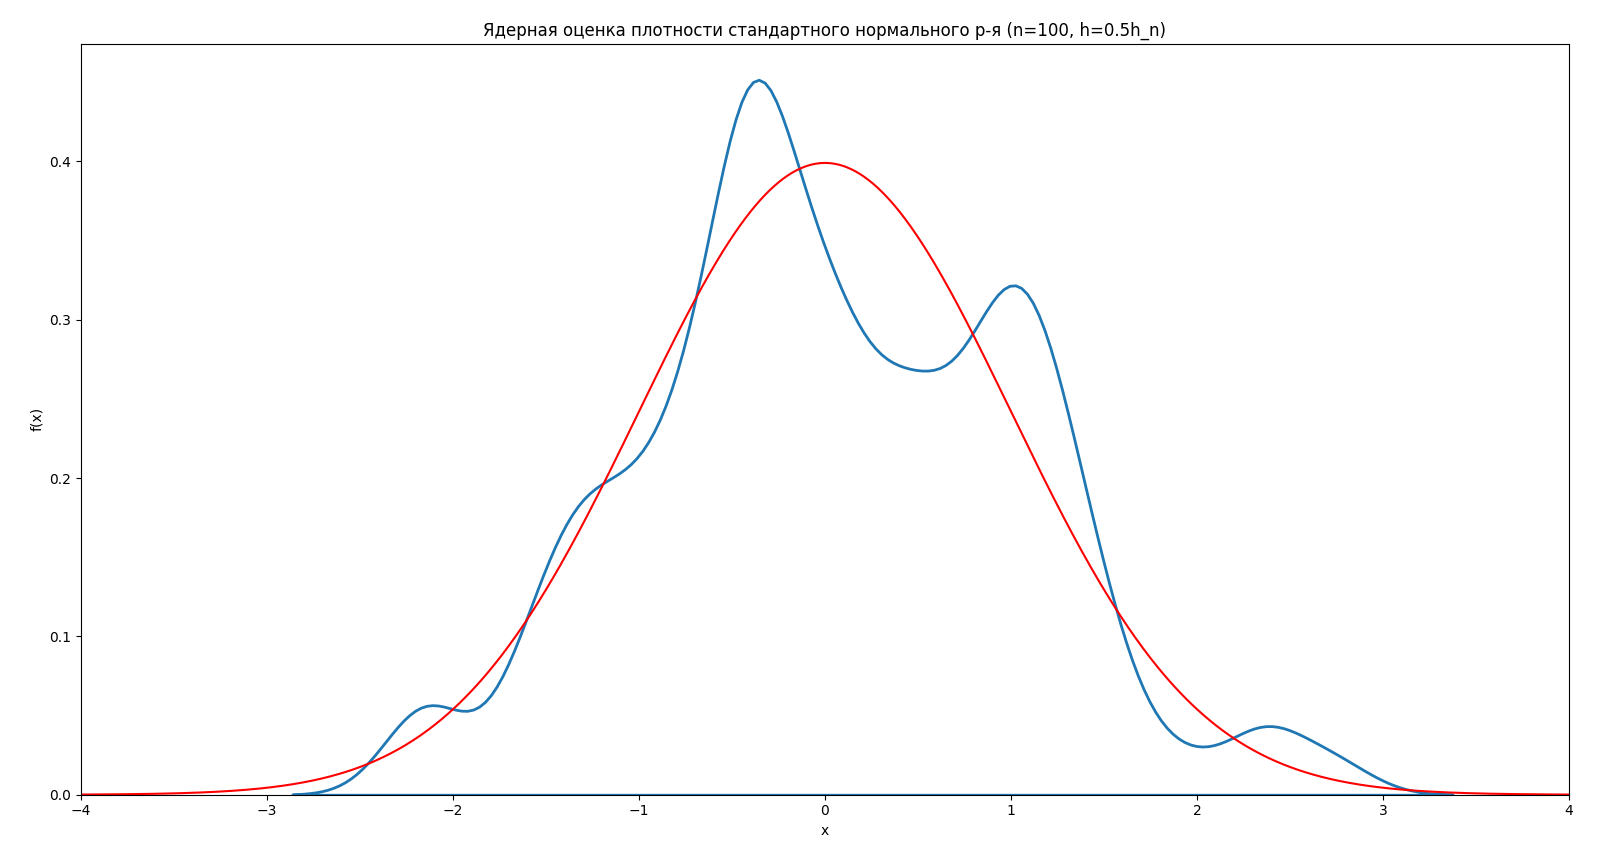
\includegraphics[scale=0.14]{resources/4_gauss_100_half.png}
		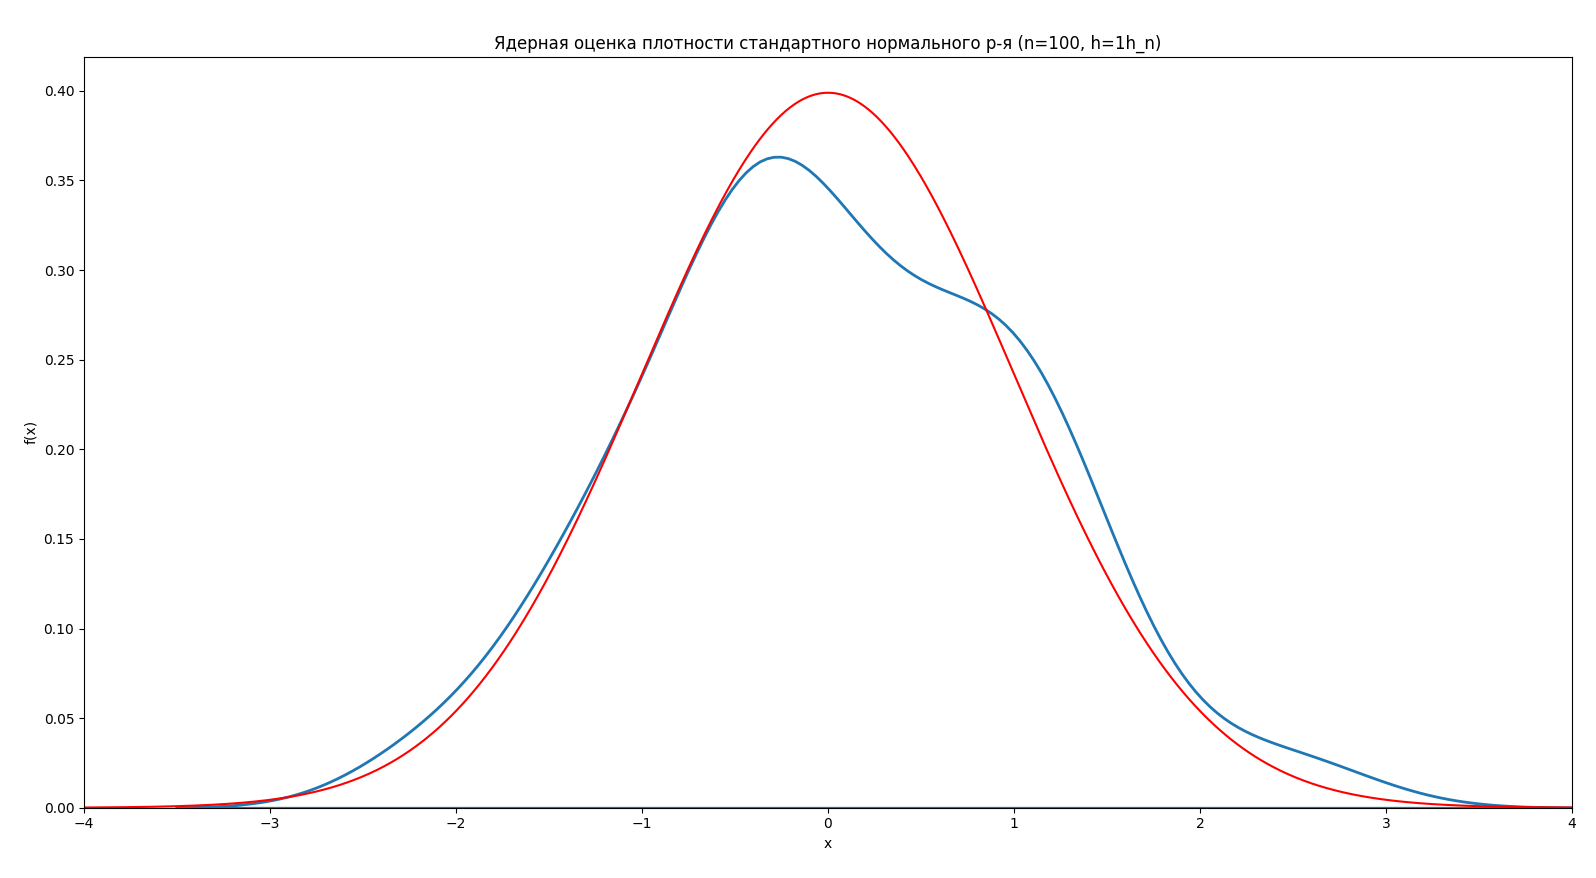
\includegraphics[scale=0.14]{resources/4_gauss_100_one.png}
		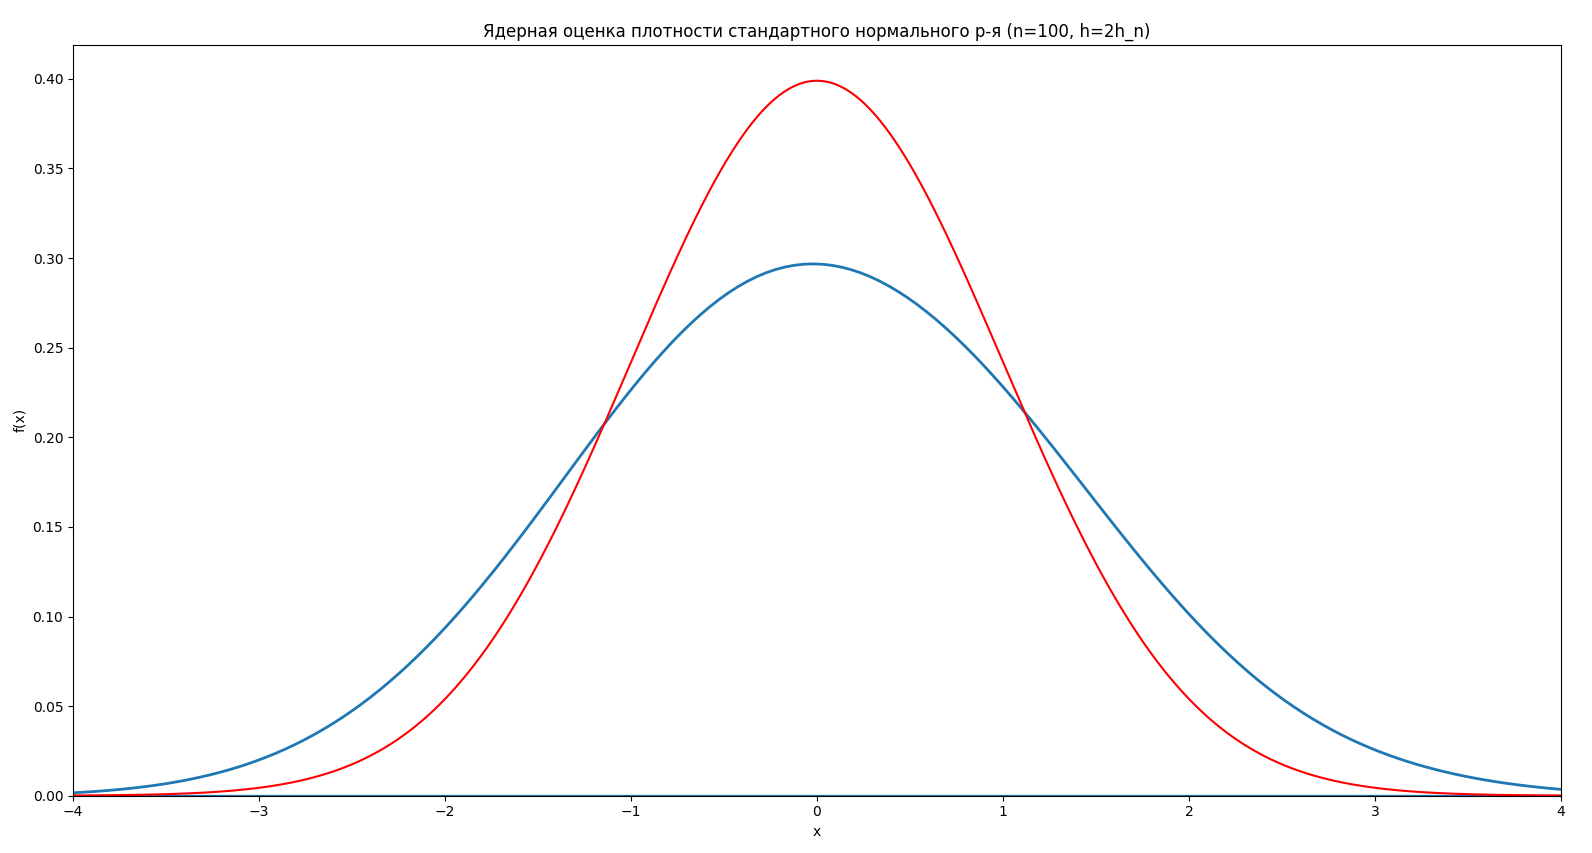
\includegraphics[scale=0.14]{resources/4_gauss_100_two.png}
	\end{tabular}
	\text{\tab \tab $h=h_{n}/2$ \tab \tab \tab \tab \tab $h=h_{n}$ \tab \tab \tab \tab \tab $h=2h_{n}$ \tab \tab }
	\caption{Нормальное распределение, $n=100$}
\end{figure}

\begin{figure}[H]
	\begin{tabular}{ccc}
		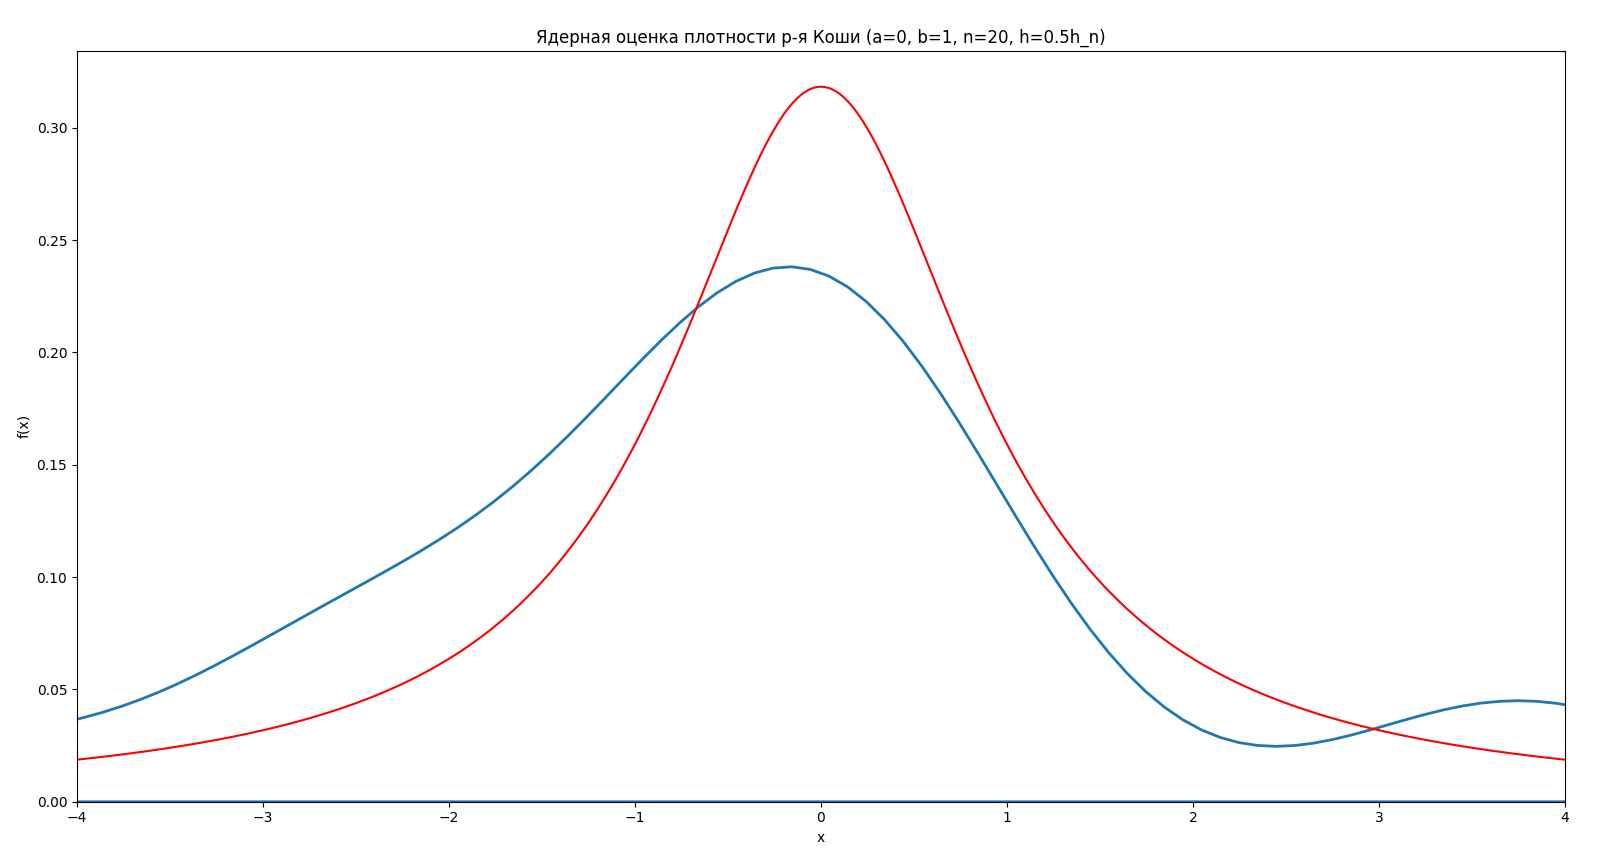
\includegraphics[scale=0.14]{resources/4_cauchy_20_half.png}
		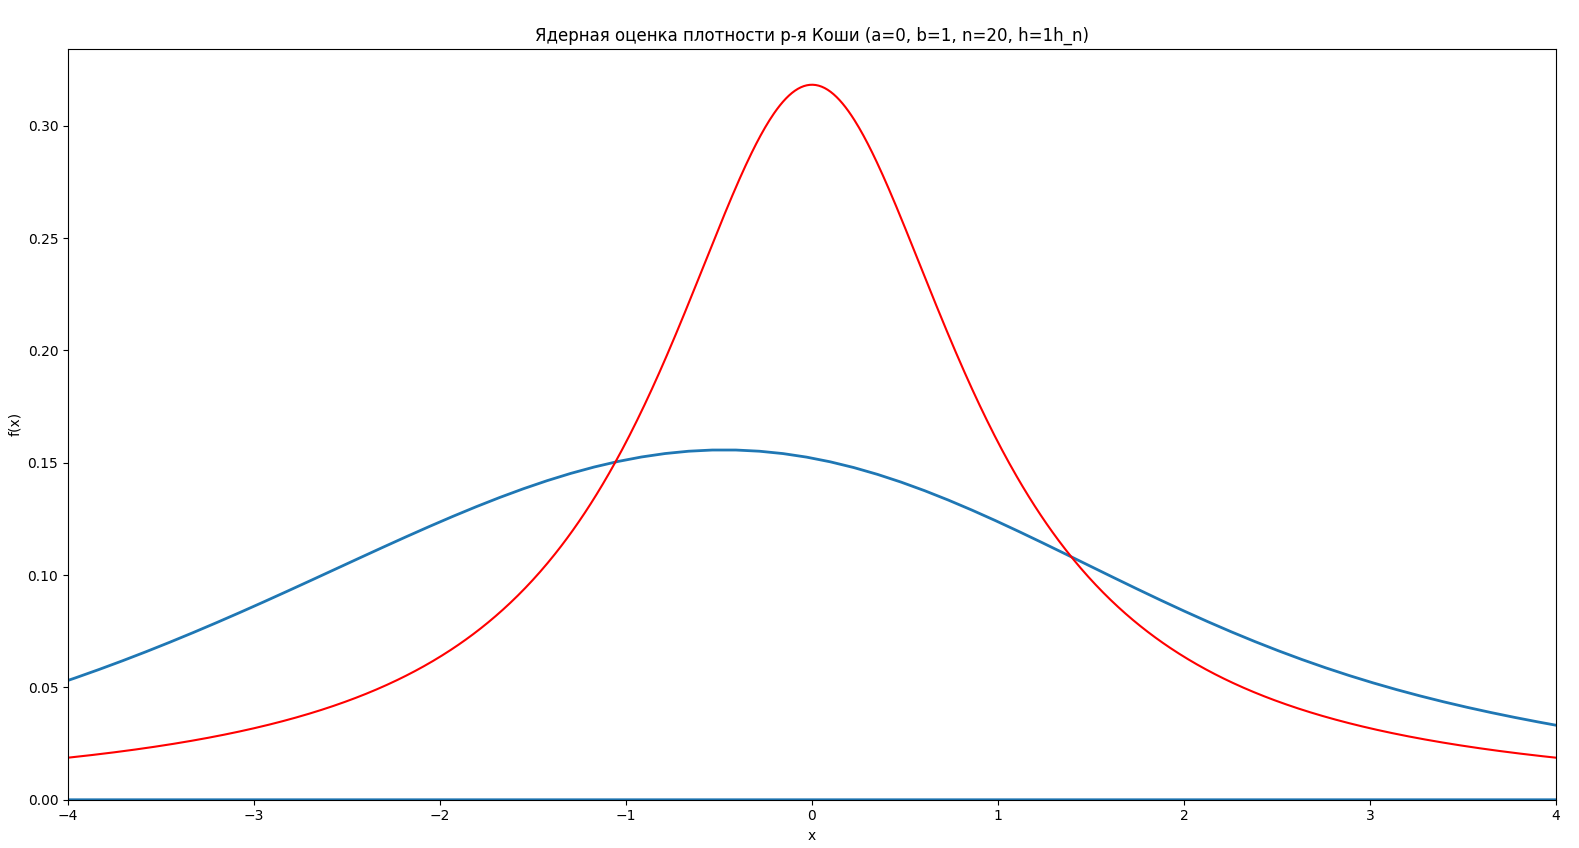
\includegraphics[scale=0.14]{resources/4_cauchy_20_one.png}
		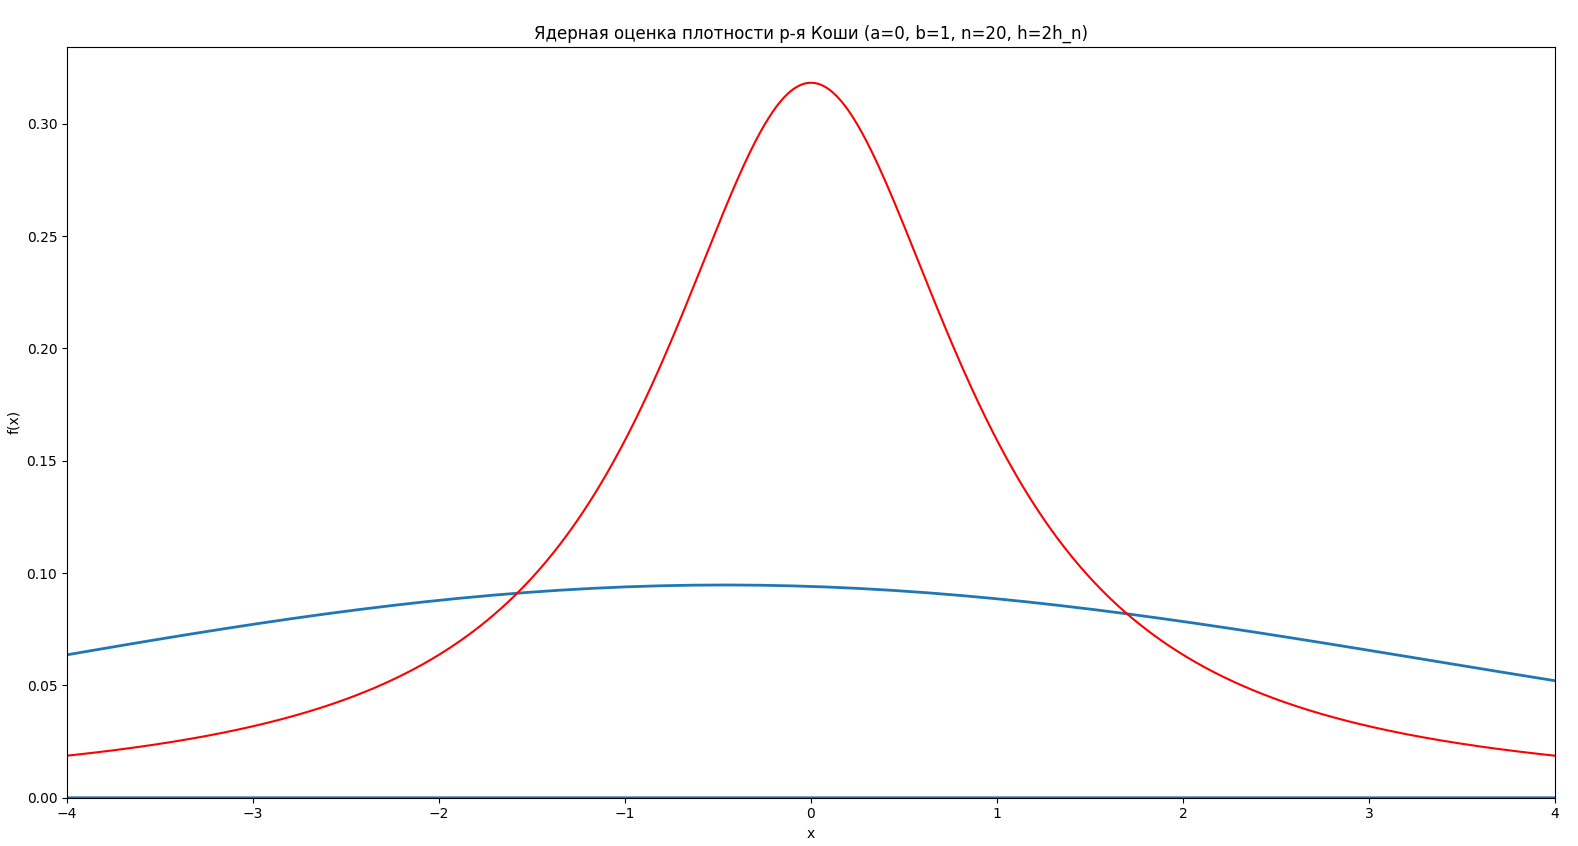
\includegraphics[scale=0.14]{resources/4_cauchy_20_two.png}
	\end{tabular}
	\text{\tab \tab $h=h_{n}/2$ \tab \tab \tab \tab \tab $h=h_{n}$ \tab \tab \tab \tab \tab $h=2h_{n}$ \tab \tab }
	\caption{Распределение Коши, $n=20$}
\end{figure}

\begin{figure}[H]
	\begin{tabular}{ccc}
		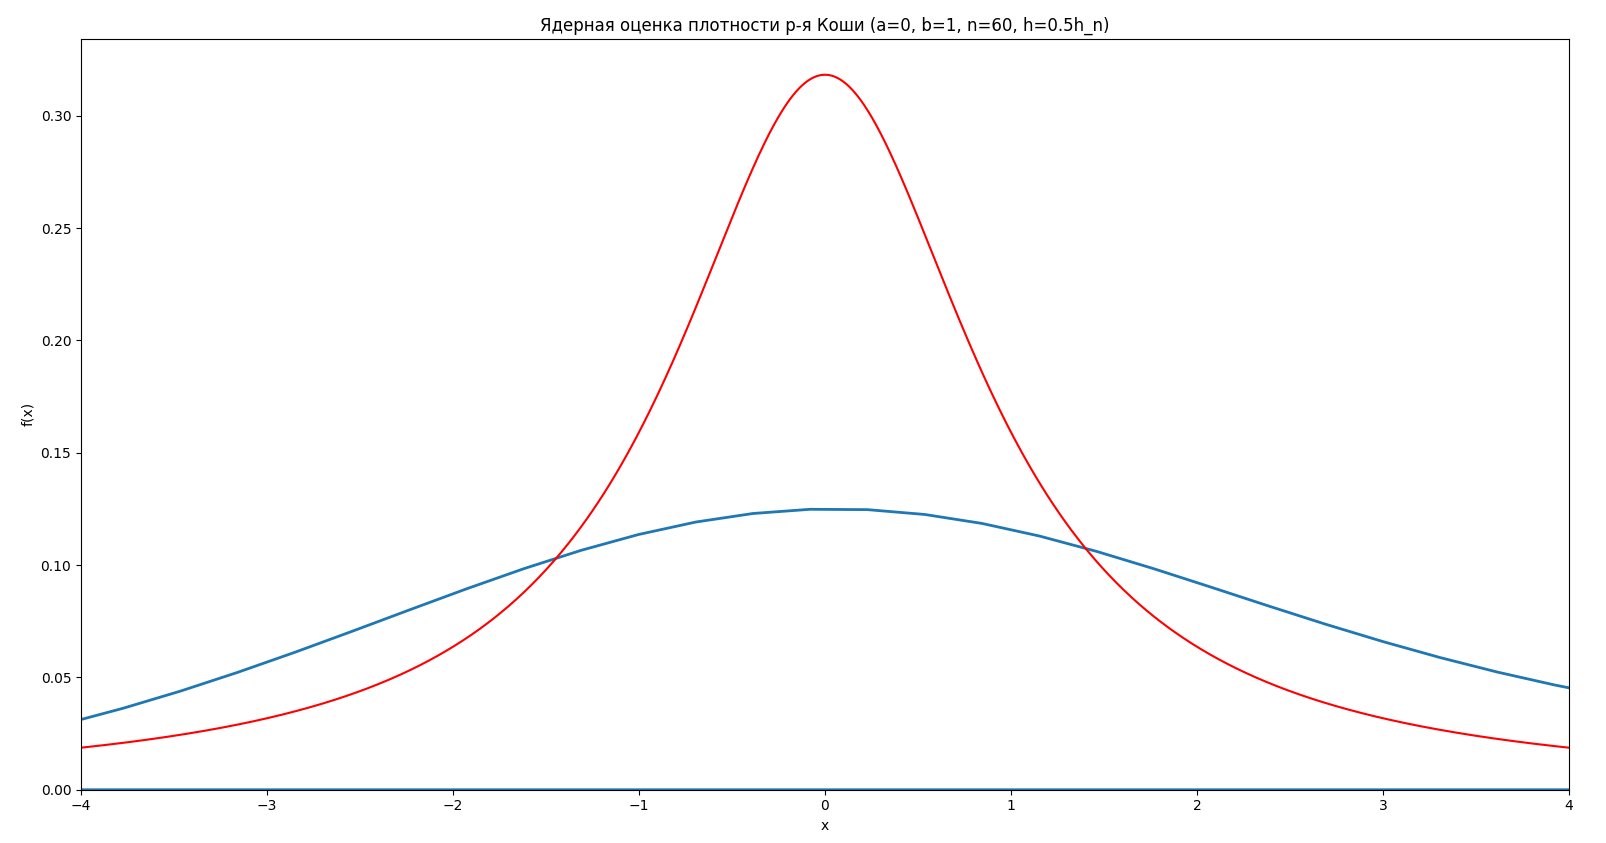
\includegraphics[scale=0.14]{resources/4_cauchy_60_half.png}
		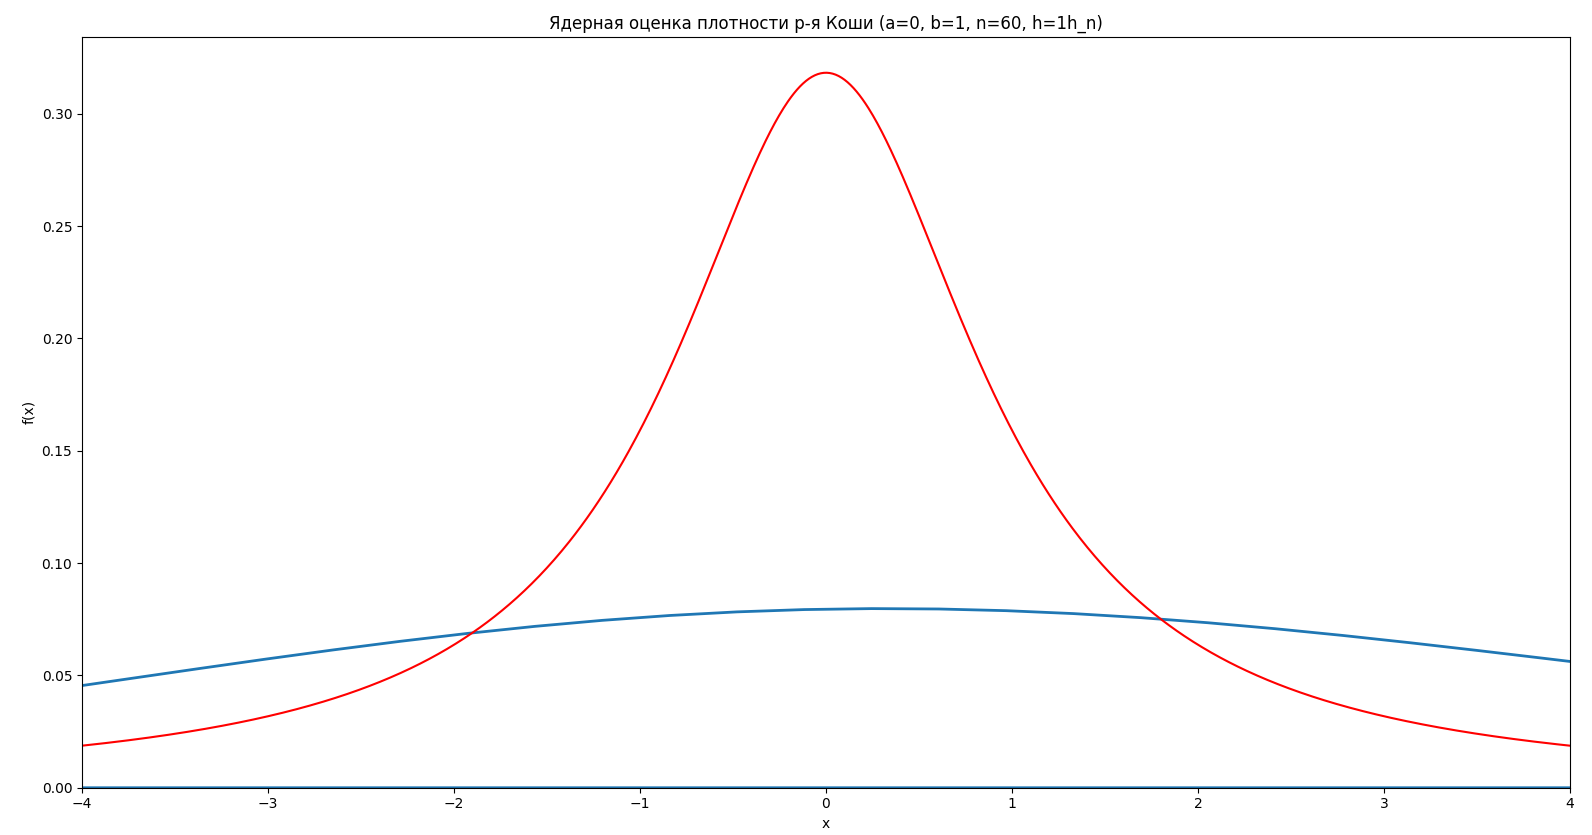
\includegraphics[scale=0.14]{resources/4_cauchy_60_one.png}
		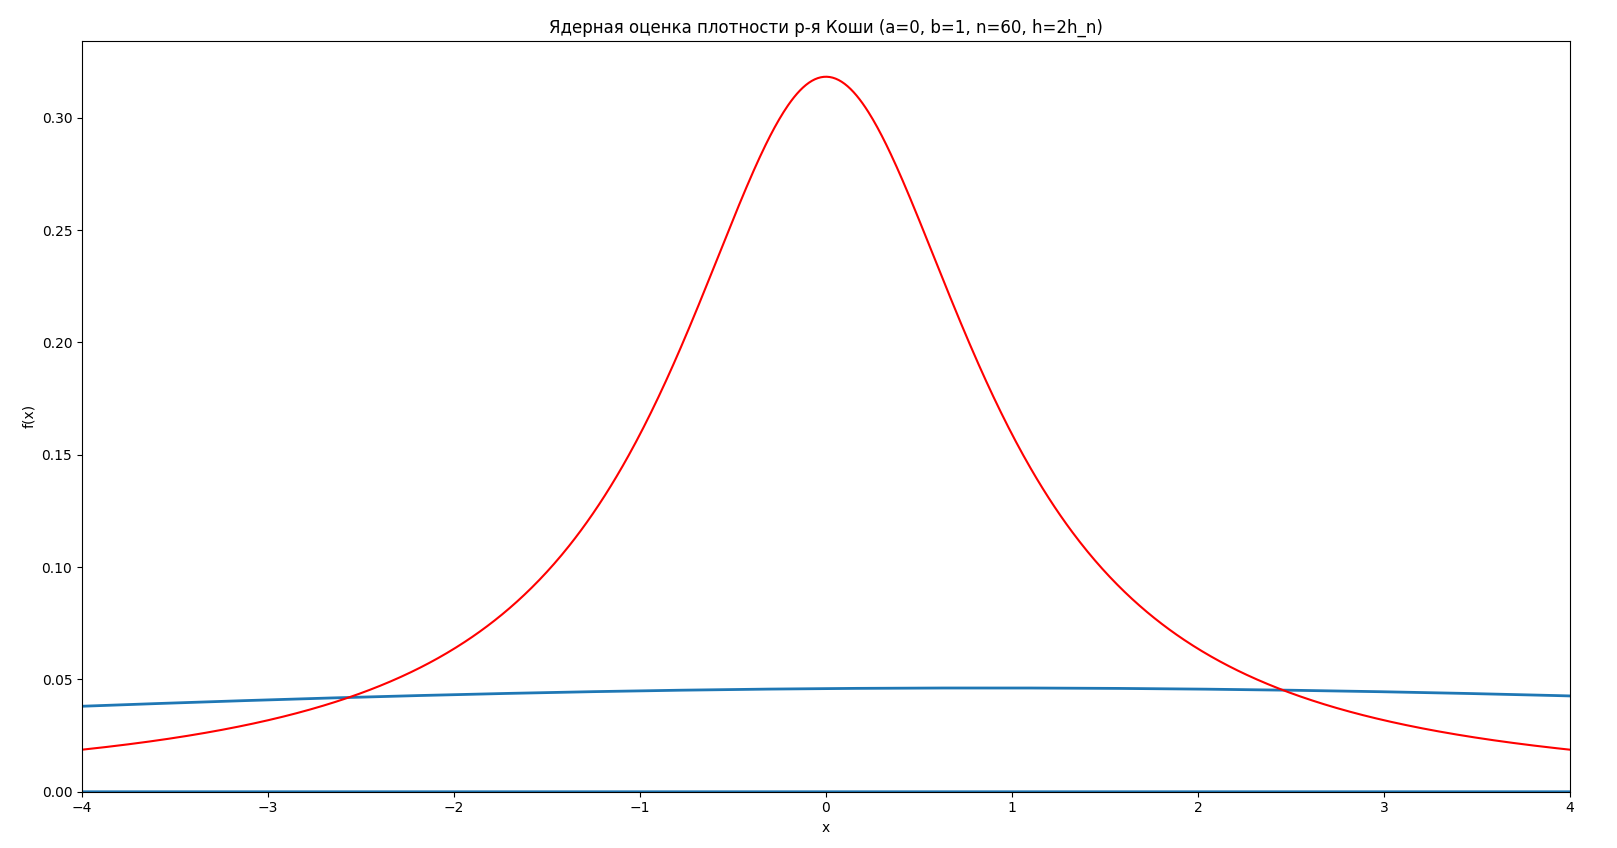
\includegraphics[scale=0.14]{resources/4_cauchy_60_two.png}
	\end{tabular}
	\text{\tab \tab $h=h_{n}/2$ \tab \tab \tab \tab \tab $h=h_{n}$ \tab \tab \tab \tab \tab $h=2h_{n}$ \tab \tab }
	\caption{Распределение Коши, $n=60$}
\end{figure}

\begin{figure}[H]
	\begin{tabular}{ccc}
		\includegraphics[scale=0.14]{resources/4_cauchy_100_half.png}
		\includegraphics[scale=0.14]{resources/4_cauchy_100_one.png}
		\includegraphics[scale=0.14]{resources/4_cauchy_100_two.png}
	\end{tabular}
	\text{\tab \tab $h=h_{n}/2$ \tab \tab \tab \tab \tab $h=h_{n}$ \tab \tab \tab \tab \tab $h=2h_{n}$ \tab \tab }
	\caption{Распределение Коши, $n=100$}
\end{figure}

\begin{figure}[H]
	\begin{tabular}{ccc}
		\includegraphics[scale=0.14]{resources/4_laplace_20_half.png}
		\includegraphics[scale=0.14]{resources/4_laplace_20_one.png}
		\includegraphics[scale=0.14]{resources/4_laplace_20_two.png}
	\end{tabular}
	\text{\tab \tab $h=h_{n}/2$ \tab \tab \tab \tab \tab $h=h_{n}$ \tab \tab \tab \tab \tab $h=2h_{n}$ \tab \tab }
	\caption{Распределение Лапласа, $n=20$}
\end{figure}

\begin{figure}[H]
	\begin{tabular}{ccc}
		\includegraphics[scale=0.14]{resources/4_laplace_60_half.png}
		\includegraphics[scale=0.14]{resources/4_laplace_60_one.png}
		\includegraphics[scale=0.14]{resources/4_laplace_60_two.png}
	\end{tabular}
	\text{\tab \tab $h=h_{n}/2$ \tab \tab \tab \tab \tab $h=h_{n}$ \tab \tab \tab \tab \tab $h=2h_{n}$ \tab \tab }
	\caption{Распределение Лапласа, $n=60$}
\end{figure}

\begin{figure}[H]
	\begin{tabular}{ccc}
		\includegraphics[scale=0.14]{resources/4_laplace_100_half.png}
		\includegraphics[scale=0.14]{resources/4_laplace_100_one.png}
		\includegraphics[scale=0.14]{resources/4_laplace_100_two.png}
	\end{tabular}
	\text{\tab \tab $h=h_{n}/2$ \tab \tab \tab \tab \tab $h=h_{n}$ \tab \tab \tab \tab \tab $h=2h_{n}$ \tab \tab }
	\caption{Распределение Лапласа, $n=100$}
\end{figure}

\begin{figure}[H]
	\begin{tabular}{ccc}
		\includegraphics[scale=0.14]{resources/4_poisson_20_half.png}
		\includegraphics[scale=0.14]{resources/4_poisson_20_one.png}
		\includegraphics[scale=0.14]{resources/4_poisson_20_two.png}
	\end{tabular}
	\text{\tab \tab $h=h_{n}/2$ \tab \tab \tab \tab \tab $h=h_{n}$ \tab \tab \tab \tab \tab $h=2h_{n}$ \tab \tab }
	\caption{Распределение Пуассона, $n=20$}
\end{figure}

\begin{figure}[H]
	\begin{tabular}{ccc}
		\includegraphics[scale=0.14]{resources/4_poisson_60_half.png}
		\includegraphics[scale=0.14]{resources/4_poisson_60_one.png}
		\includegraphics[scale=0.14]{resources/4_poisson_60_two.png}
	\end{tabular}
	\text{\tab \tab $h=h_{n}/2$ \tab \tab \tab \tab \tab $h=h_{n}$ \tab \tab \tab \tab \tab $h=2h_{n}$ \tab \tab }
	\caption{Распределение Пуассона, $n=60$}
\end{figure}

\begin{figure}[H]
	\begin{tabular}{ccc}
		\includegraphics[scale=0.14]{resources/4_poisson_100_half.png}
		\includegraphics[scale=0.14]{resources/4_poisson_100_one.png}
		\includegraphics[scale=0.14]{resources/4_poisson_100_two.png}
	\end{tabular}
	\text{\tab \tab $h=h_{n}/2$ \tab \tab \tab \tab \tab $h=h_{n}$ \tab \tab \tab \tab \tab $h=2h_{n}$ \tab \tab }
	\caption{Распределение Пуассона, $n=100$}
\end{figure}

\begin{figure}[H]
	\begin{tabular}{ccc}
		\includegraphics[scale=0.14]{resources/4_uniform_20_half.png}
		\includegraphics[scale=0.14]{resources/4_uniform_20_one.png}
		\includegraphics[scale=0.14]{resources/4_uniform_20_two.png}
	\end{tabular}
	\text{\tab \tab $h=h_{n}/2$ \tab \tab \tab \tab \tab $h=h_{n}$ \tab \tab \tab \tab \tab $h=2h_{n}$ \tab \tab }
	\caption{Равномерное распределение, $n=20$}
\end{figure}

\begin{figure}[H]
	\begin{tabular}{ccc}
		\includegraphics[scale=0.14]{resources/4_uniform_60_half.png}
		\includegraphics[scale=0.14]{resources/4_uniform_60_one.png}
		\includegraphics[scale=0.14]{resources/4_uniform_60_two.png}
	\end{tabular}
	\text{\tab \tab $h=h_{n}/2$ \tab \tab \tab \tab \tab $h=h_{n}$ \tab \tab \tab \tab \tab $h=2h_{n}$ \tab \tab }
	\caption{Равномерное распределение, $n=60$}
\end{figure}

\begin{figure}[H]
	\begin{tabular}{ccc}
		\includegraphics[scale=0.14]{resources/4_uniform_100_half.png}
		\includegraphics[scale=0.14]{resources/4_uniform_100_one.png}
		\includegraphics[scale=0.14]{resources/4_uniform_100_two.png}
	\end{tabular}
	\text{\tab \tab $h=h_{n}/2$ \tab \tab \tab \tab \tab $h=h_{n}$ \tab \tab \tab \tab \tab $h=2h_{n}$ \tab \tab }
	\caption{Равномерное распределение, $n=100$}
\end{figure}

\newpage
